\documentclass[a4paper, 11pt]{article}

\usepackage{misc-macros}
\usepackage{tabularx}
\usepackage{caption}
\usepackage[bottom]{footmisc}

\newcounter{capfn}

\setmainfont{C059}
\setmonofont{Jet Brains Mono}[Ligatures=TeX, Scale=MatchLowercase]

\begin{document}
	
	\thispagestyle{empty}
	
	\begin{center}
		
		\setstretch{2}
		
		\vspace*{1cm}
		
		{\huge\bfseries \ifnt{Among the Canopy}\\[2.5em]
			An Educational Visit to Karnala Bird Sanctuary and Yusuf Meherally Center }
		
		\vspace*{3cm}
		
		\LARGE \ul{Date of visit}: \nth{22} August 2026.\\[1em]
		\ul{Date of report}: \today.\\
		
		\vfill
		
		{\setstretch{1}
		
		\bfnt{Wrichik Basu}\\
		SY BSc CS\\
		\texttt{SCS2627067}\\}
		
		
	\end{center}
	
	\clearpage
	
	\setcounter{page}{1}
	\pagestyle{frontmatter}
	
	\tableofcontents
	\listoffigures
	
	\clearpage
	
	\setcounter{page}{1}
	\pagestyle{regular}
	
	\section{Itinerary}
	
		\begin{center}
			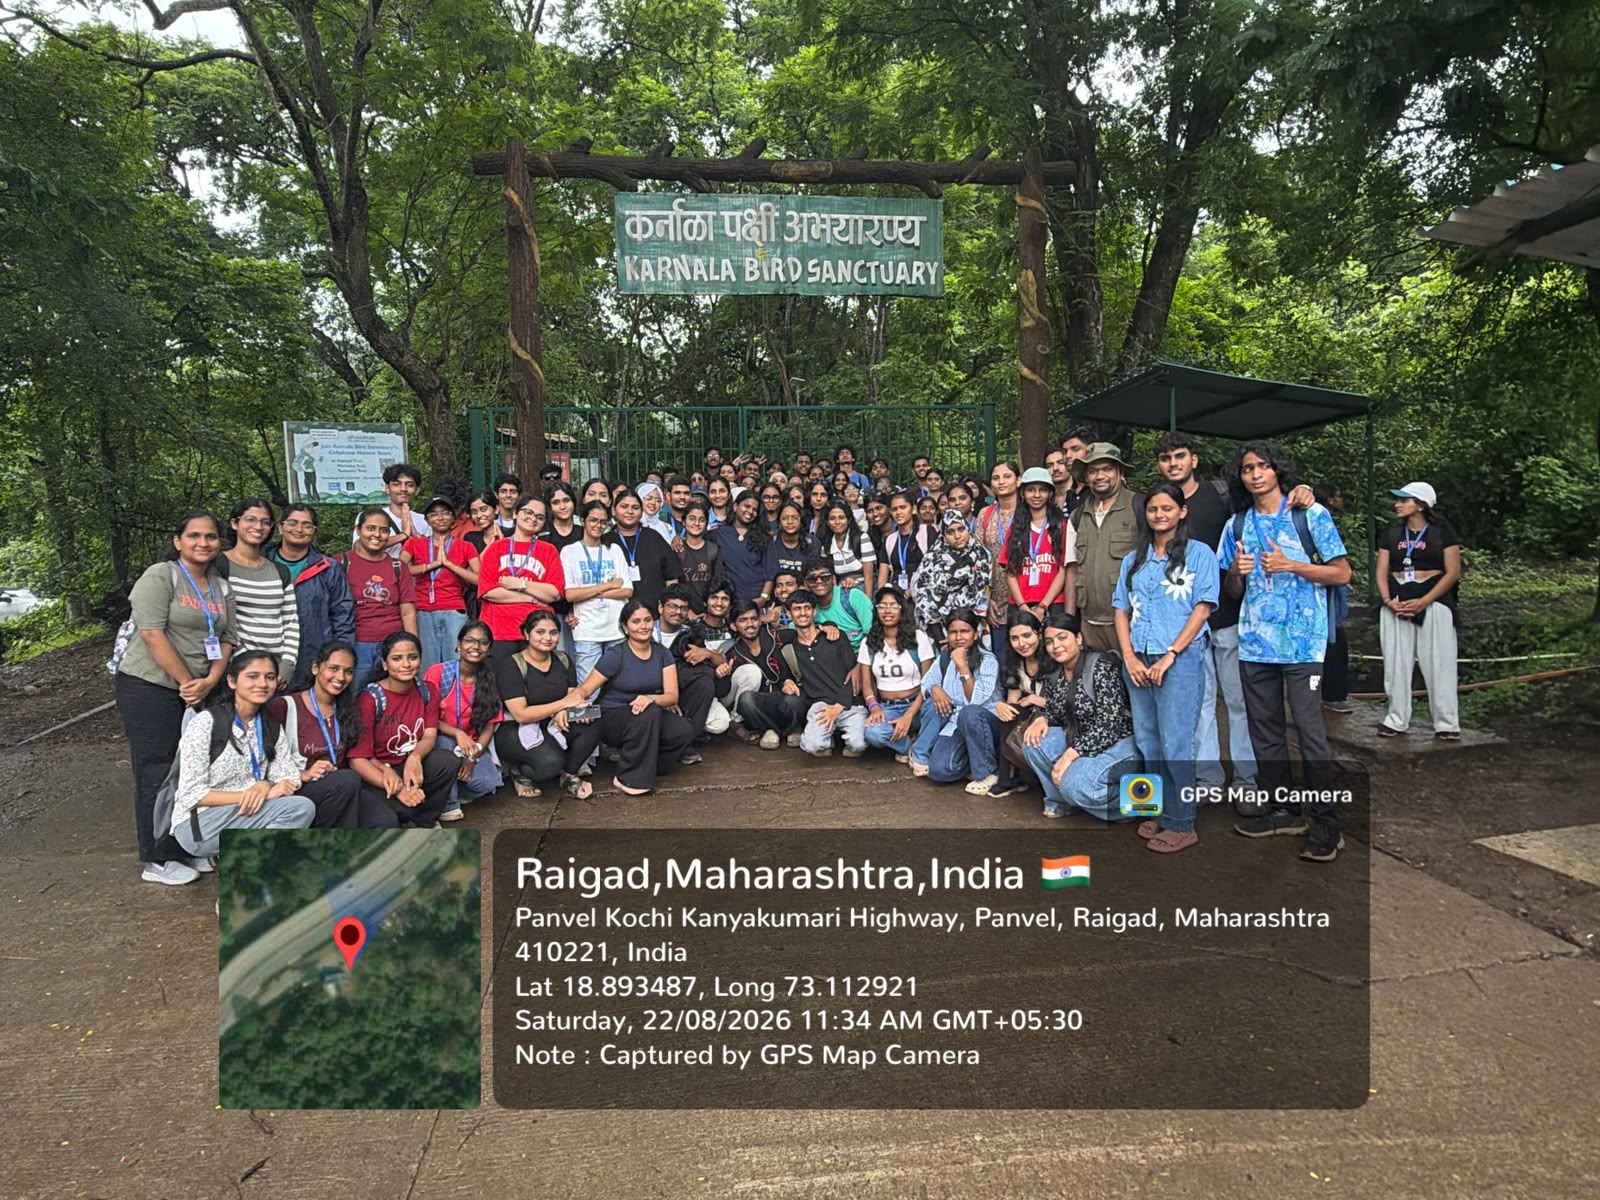
\includegraphics[width=0.9\textwidth]{group_photo_entrance.jpg}
			\captionof{figure}{Group photo taken at the entrance of the Karnala Bird Sanctuary.}
		\end{center}
		
		The education field excursion was arranged under the leadership of Dr. Vishnuprasad, Head of Department, Dept. of Environmental Sciences. The itinerary followed was as follows:\\
		
		\begin{tabularx}{\textwidth}{l>{\raggedright\arraybackslash}X}
			
			06:45~AM & Arrival at college, signing the attendance register\\
			
			07:40~AM & Departure from college (delayed due to rain and delayed arrival of transport) \\
			
			09:40~AM & Arrival at Yusuf Meherally Center\\
			
			10:30~AM & Breakfast and tea over, heading to Karnala Bird Sanctuary after briefing\\
			
			11:00~AM & Reach gate of bird sanctuary\\
			
			11:40~AM & Start excursion after ticket purchase, bag checking, briefing by faculty about Do's and Don'ts inside the reserve forest\\
			
			02:00~PM & Exit from sanctuary, bag-check, travel back to Yusuf Meherally Center, lunch\\
			
			03:20~PM & Start of guided trip of small-scale industries in Yusuf Meherally Center\\
			
			04:45~PM & End of tour, evening tea \& snacks\\
			
			05:40~PM & Bid adieu to Yusuf Meherally Center and the greenery\\
			
			07:40~PM & Drop at college.
			
		\end{tabularx}
	
	\section{Karnala Bird Sanctuary}
	
	\begin{center}
		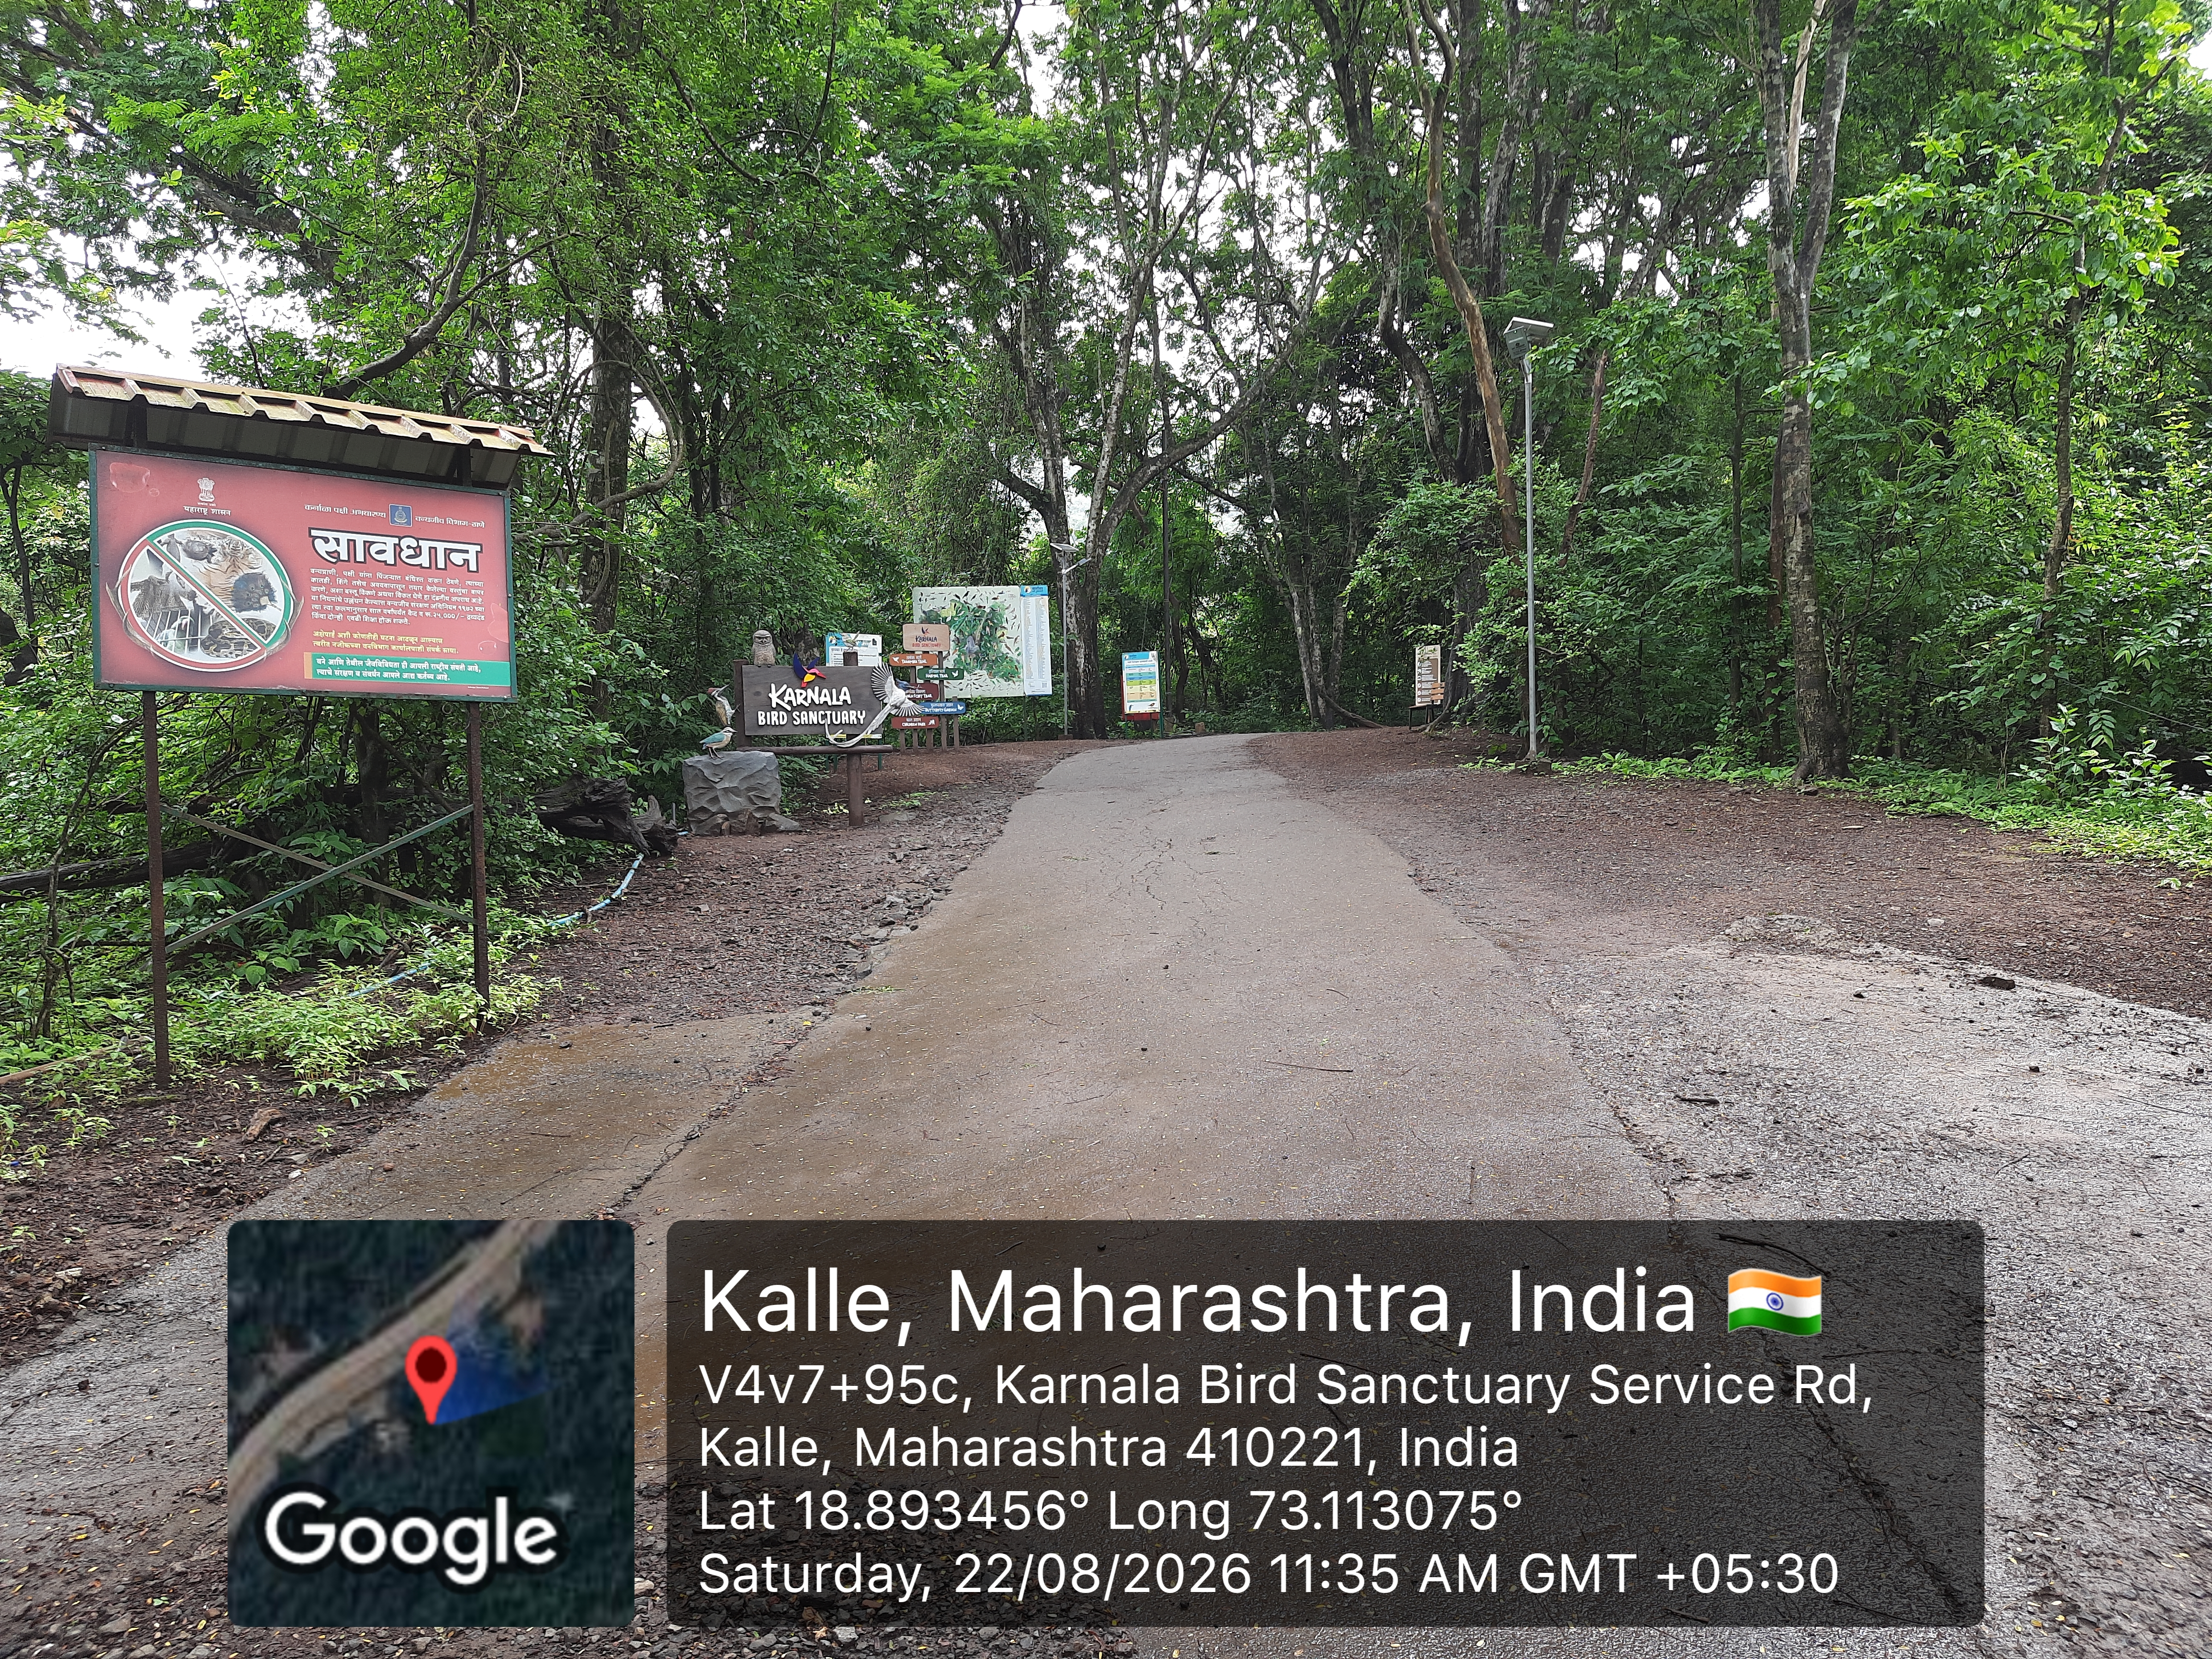
\includegraphics[width=0.7\textwidth]{karnala_entrance.jpg}
		\captionof{figure}{Inside the gates of Karnala Bird Sanctuary.}
	\end{center}
	
	The Karnala Bird Sanctuary is located on NH~66, in the Panvel taluk of Raigad (erstwhile Raigarh) district of Maharashtra, around \SI{54}{km} from Mumbai. The area is centred around the Karnala Fort, and occupies an area of \SI{12.11}{sq. km}.\\
	
	Survey of India maps this area under the topographic map \texttt{47F/1} or Open Series Map \texttt{E43H1}. The area has been demarcated as a Reserve Forest, though current official records categorises the area as IUCN category -- IV (habitat/species management area). The relevant portion of the topo map can be seen in figure~\ref{fig:topo}. The calculated latitude and longitude of the officially demarcated entrance of the Wildlife Sanctuary is $\ang{18;53;41.604}N$, $\ang{73;6;54.0822}E$. The ruins of the Karnala Fort bear coordinates $\ang{18;52;55.5744}N$, $\ang{73;7;0.9144}E$. These, along with the contours of this region, are in figure~\ref{fig:topo}.\\
	
	The sanctuary, though small in area, is home to over 222 species of birds, of which 161 are resident species. The following species endemic to the Western Ghats have been found here:%
	%	
	\begin{enumerate}
		
		\item \ifnt{Treron affinis} (grey-fronted green pigeon);
		
		\item \ifnt{Columba elphinstonii} (Nilgiri woodpigeon);
		
		\item \ifnt{Pisttacula columbodies} (Malabar blue-winged parakeet);
		
		\item \ifnt{Ocyceros griseus} (Malabar grey hornbill);
		
		\item \ifnt{Megalamia viridis} (white-cheeked barbet);
		
		\item \ifnt{Galerida malabarica} (Malabar lark);
		
		\item \ifnt{Leptocoma minima} (Small Sunbird); and 
		
		\item \ifnt{Aethopyga vigorsii} (Vigor's Sunbird).
		
	\end{enumerate}
	
	The Sanctuary is also an Important Bird Area (IBA) satisfying A1 (Globally threatened species) and A2 (Restricted-range species) criteria. The sanctuary is also home to 114 species of butterflies.
	
	\begin{center}
		\begin{minipage}{0.45\textwidth}
			\centering
			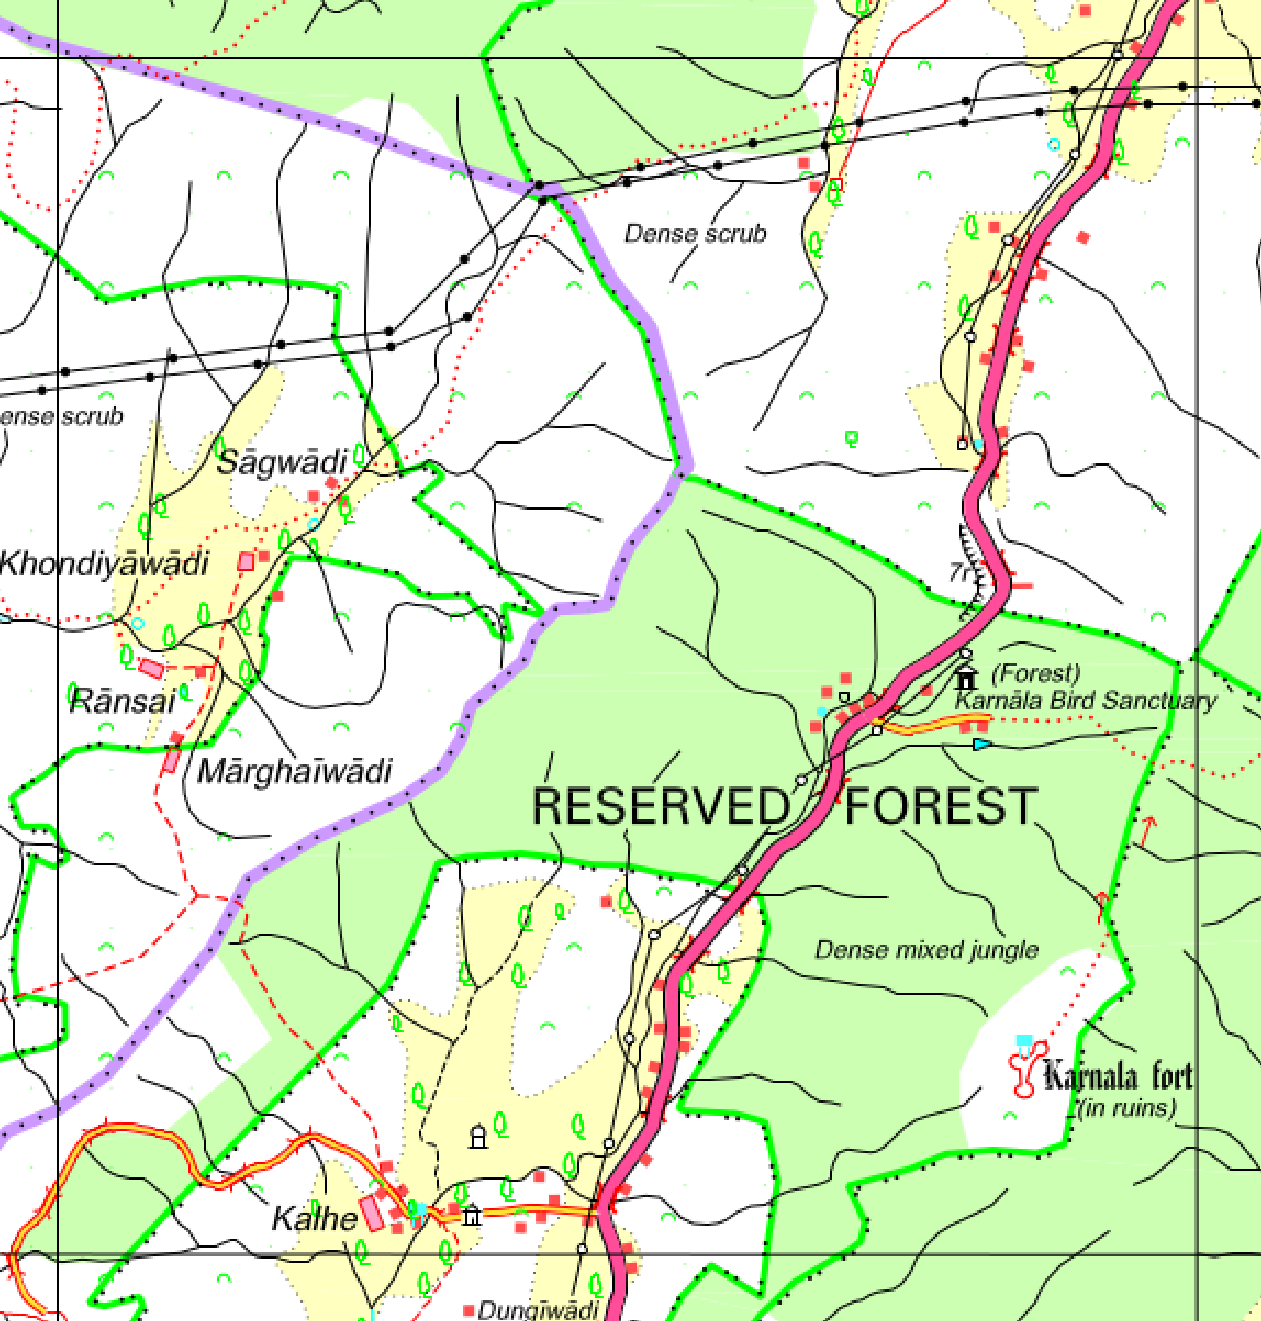
\includegraphics[width=\linewidth]{karnala_topo.png}
		\end{minipage}\hfill%
		\begin{minipage}{0.5\textwidth}
			\centering
			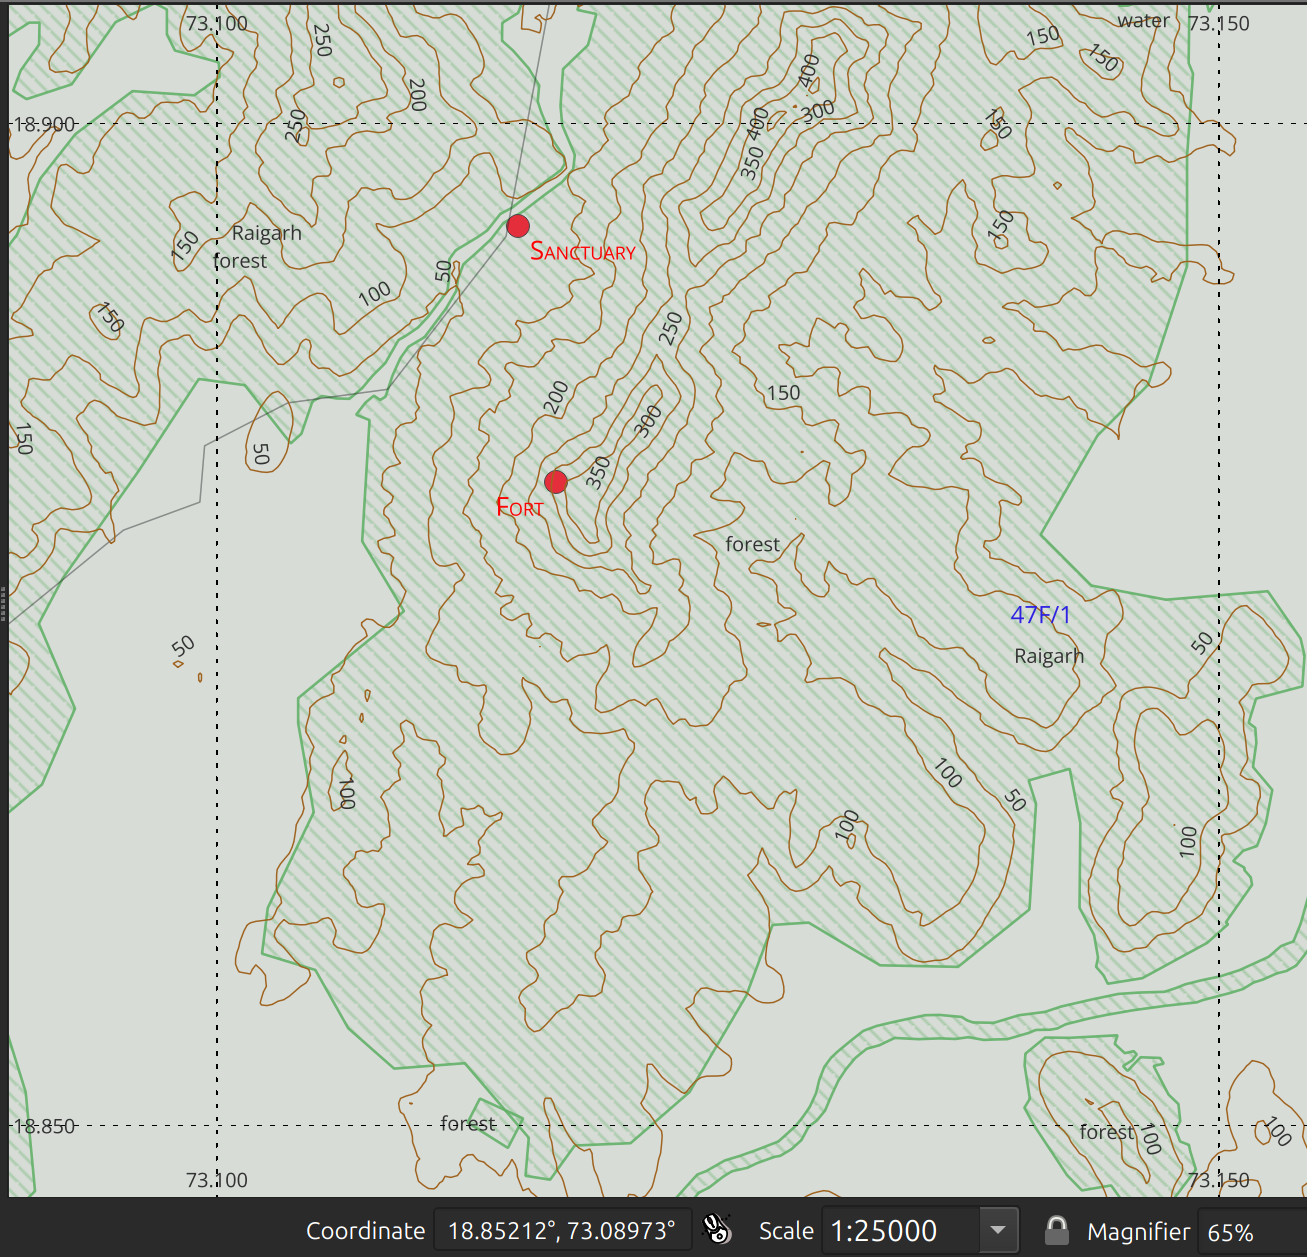
\includegraphics[width=\linewidth]{map_export.png}
		\end{minipage}
		
		\setcounter{capfn}{\value{footnote}}%
		\captionof{figure}[Karnala on topo map]{\label{fig:topo}%
			Left: Karnala Bird Sanctuary and Karnala Fort on topo map no.\ \texttt{47F/1}
			a.k.a. OSM no.\ \texttt{E43H1}. Right: Same region on QGIS software.
			The district information has been taken from
			GADM.org\footnotemark[\numexpr\value{capfn}+1\relax];
			natural area layer is from BBBike
			extract\footnotemark[\numexpr\value{capfn}+2\relax].
			Due to the National Map Policy of 2005, Open Series maps published by the
			Survey of India do not have contours, citing restrictions due to national
			security. Contour data has hence been extracted from
			OpenTopography\footnotemark[\numexpr\value{capfn}+3\relax].
			The OSM Index has been taken from Survey of
			India\footnotemark[\numexpr\value{capfn}+4\relax].}%
		%
		\stepcounter{capfn}\footnotetext[\value{capfn}]{\url{https://gadm.org/download_country.html}}%
		\stepcounter{capfn}\footnotetext[\value{capfn}]{\url{https://download2.bbbike.org/osm/extract/planet_73.02,18.817_73.237,18.965.osm.shp.zip}}%
		\stepcounter{capfn}\footnotetext[\value{capfn}]{\url{https://opentopography.org/}}%
		\stepcounter{capfn}\footnotetext[\value{capfn}]{\url{https://onlinemaps.surveyofindia.gov.in/FreeMapSpecification.aspx}}%
		\setcounter{footnote}{\value{capfn}}%
	\end{center}
	
		\subsection{Objectives of visit}
		
		\begin{itemize}
			
			\item \bfnt{Biodiversity and ecosystem study:} The sanctuary is a patch of moist deciduous and semi-evergreen forest in the Western Ghats foothills. This lets students see how a forest ecosystem functions as a whole, including the interdependence of flora and fauna, food chains and food webs, and the role of habitat in supporting species.
			
			\item \bfnt{Ornithological study:} Karnala is known primarily as a bird sanctuary, so the central purpose is observing avian diversity in a natural setting. Students can learn field identification of resident and migratory species, study bird behaviour, calls, feeding patterns, and nesting, and understand the difference between observing birds in the wild versus reading about them.
			
			\item \bfnt{Understanding conservation and protected areas:} A sanctuary is a legally protected area, so a visit teaches the purpose and functioning of such protected zones, the threats they face (habitat loss, human encroachment, poaching), and why conservation matters. It connects classroom concepts of environmental protection to a real, managed site.
			
			\item \bfnt{Field methodology and observation skills:} Trips like this train students in the practical side of science: recording observations, using binoculars and field guides, maintaining a field notebook, sketching or photographing specimens, and learning patience and discipline in data collection.
			
			\item \bfnt{Ecology and environmental awareness:} Direct exposure to a natural habitat builds sensitivity toward environmental issues and the value of the Western Ghats as a biodiversity hotspot. It reinforces concepts of sustainability and the human impact on ecosystems.
			
		\end{itemize}
		
		\subsection{Observations: Flora, fauna, and abiotic features}
			
		\begin{center}
			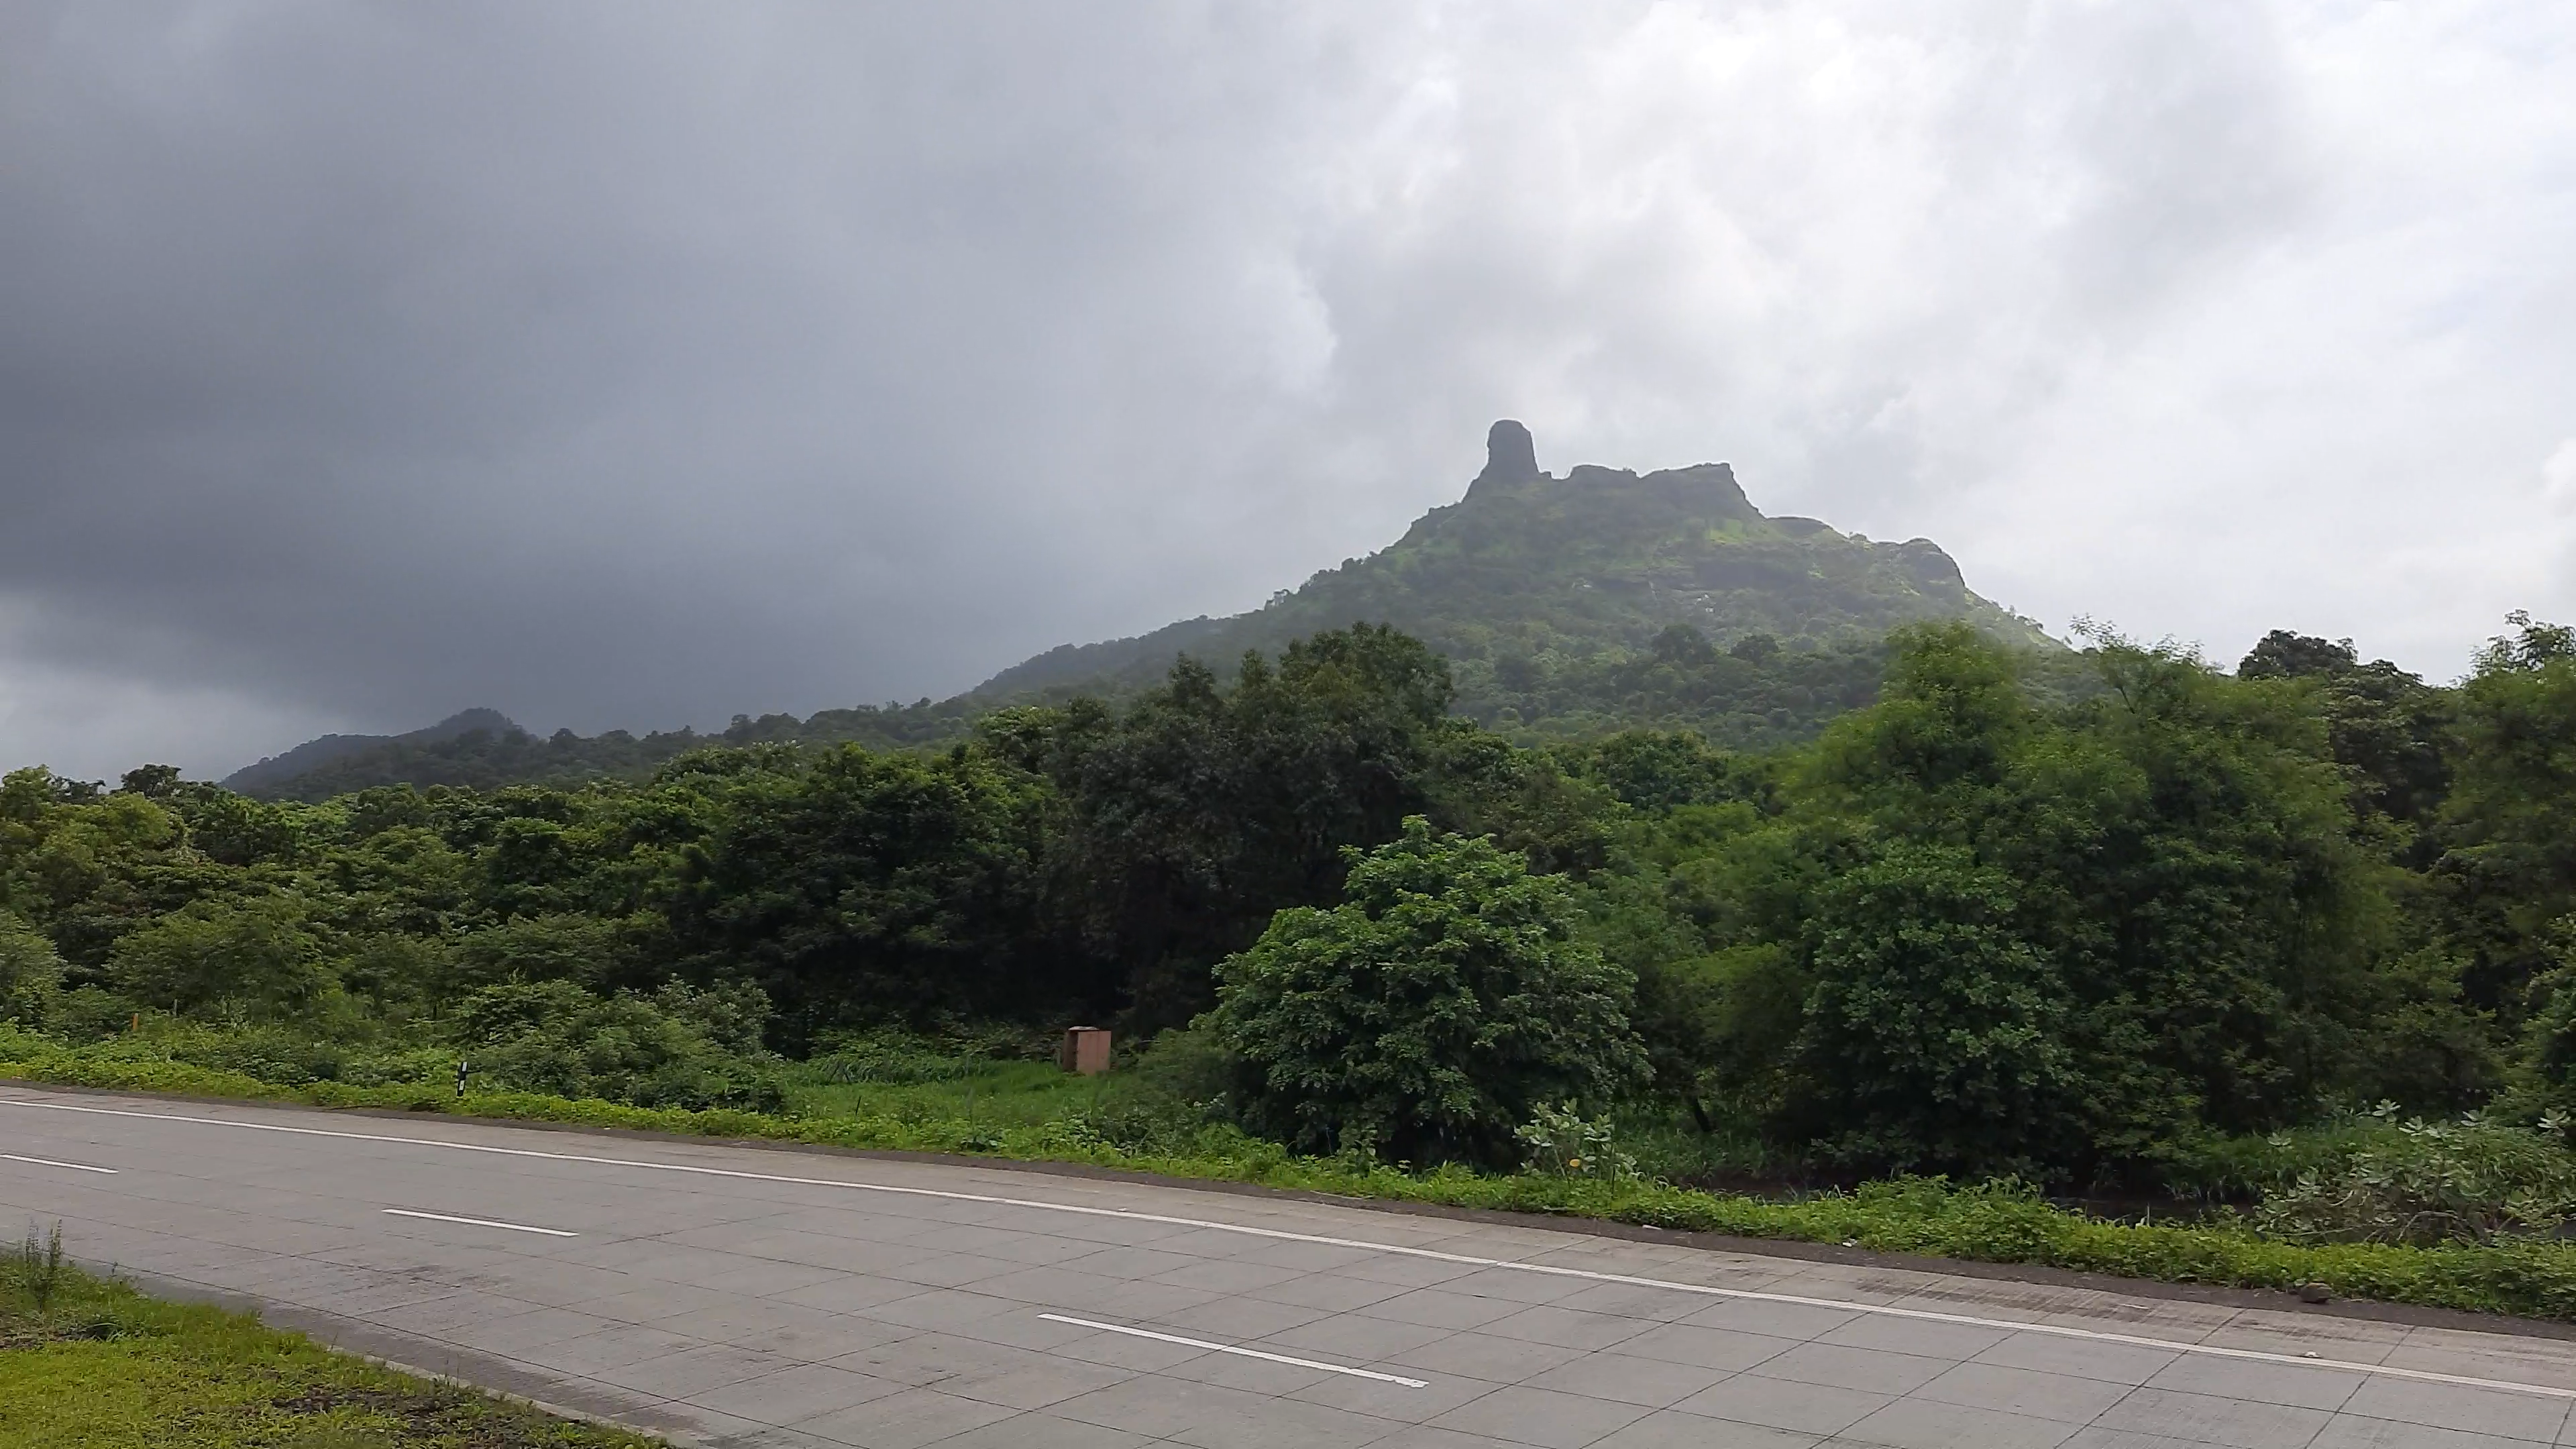
\includegraphics[width=0.8\textwidth]{karnala_fort_nh66.png}
			\captionof{figure}{Karnala Fort pinnacle seen from NH~66.}
			
			\vspace*{1cm}
			
			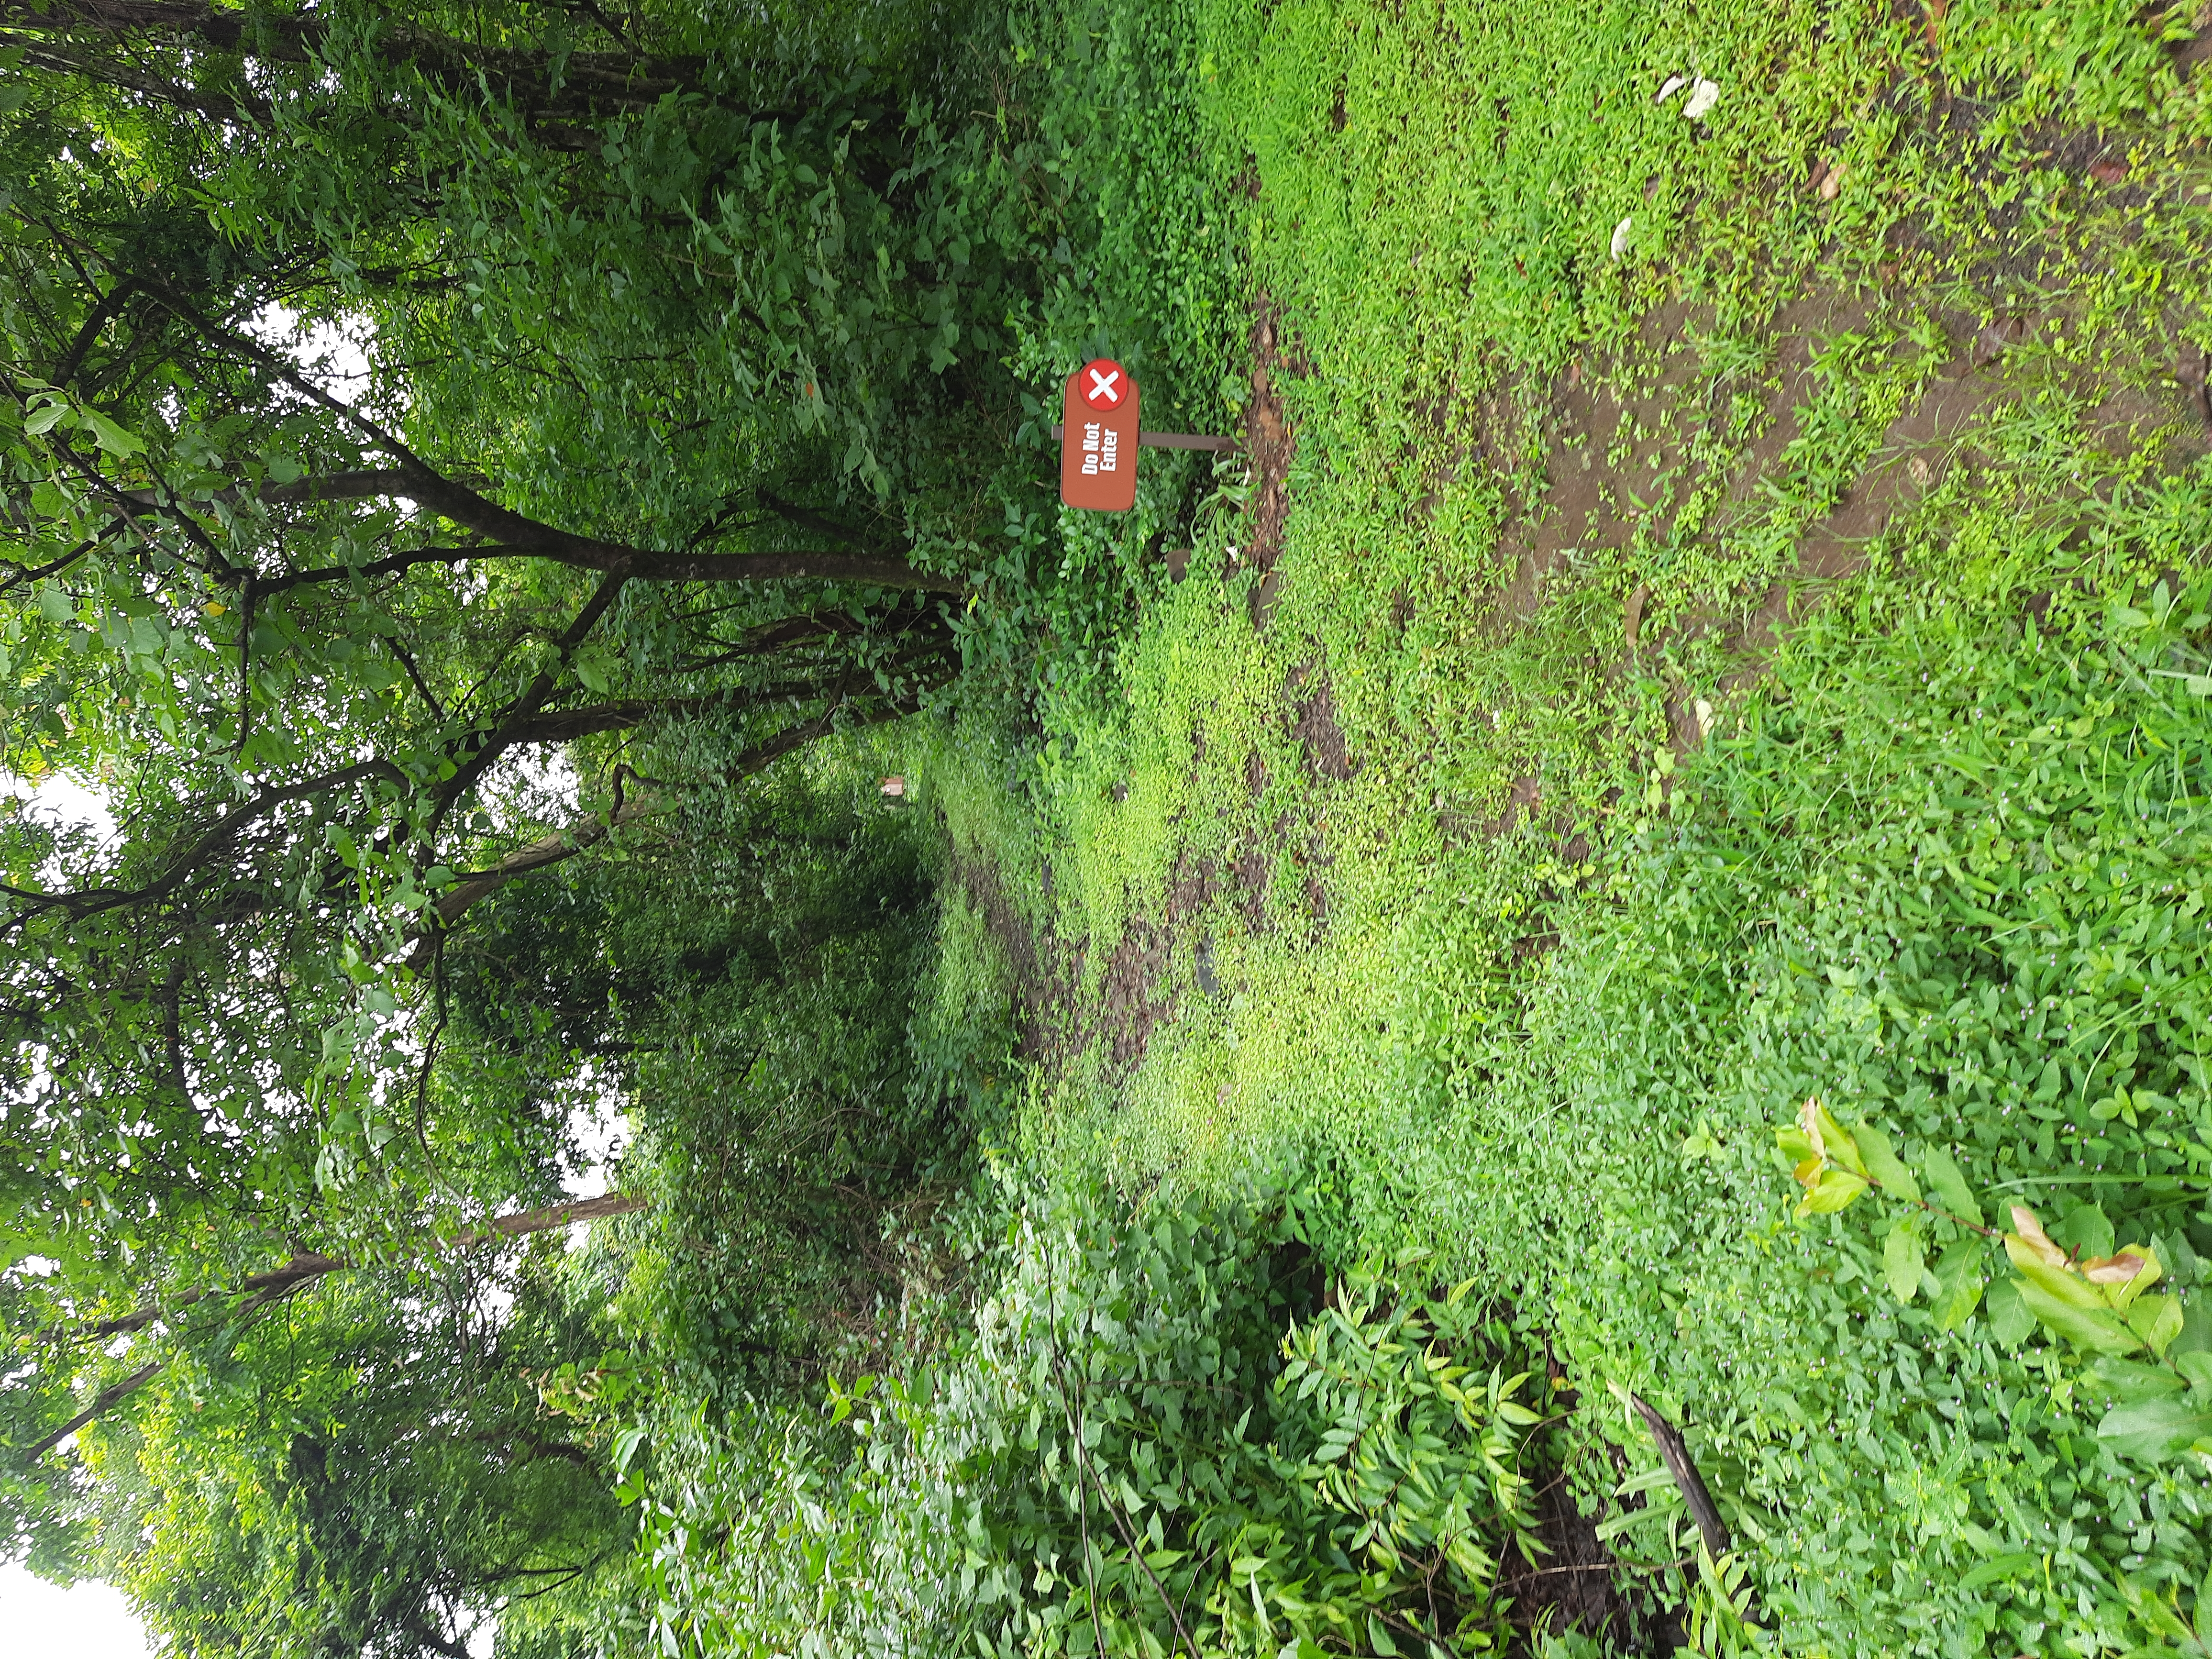
\includegraphics[height=0.6\textwidth,angle=-90]{jungle_route.jpg}
		\end{center}
		
		\begin{center}
			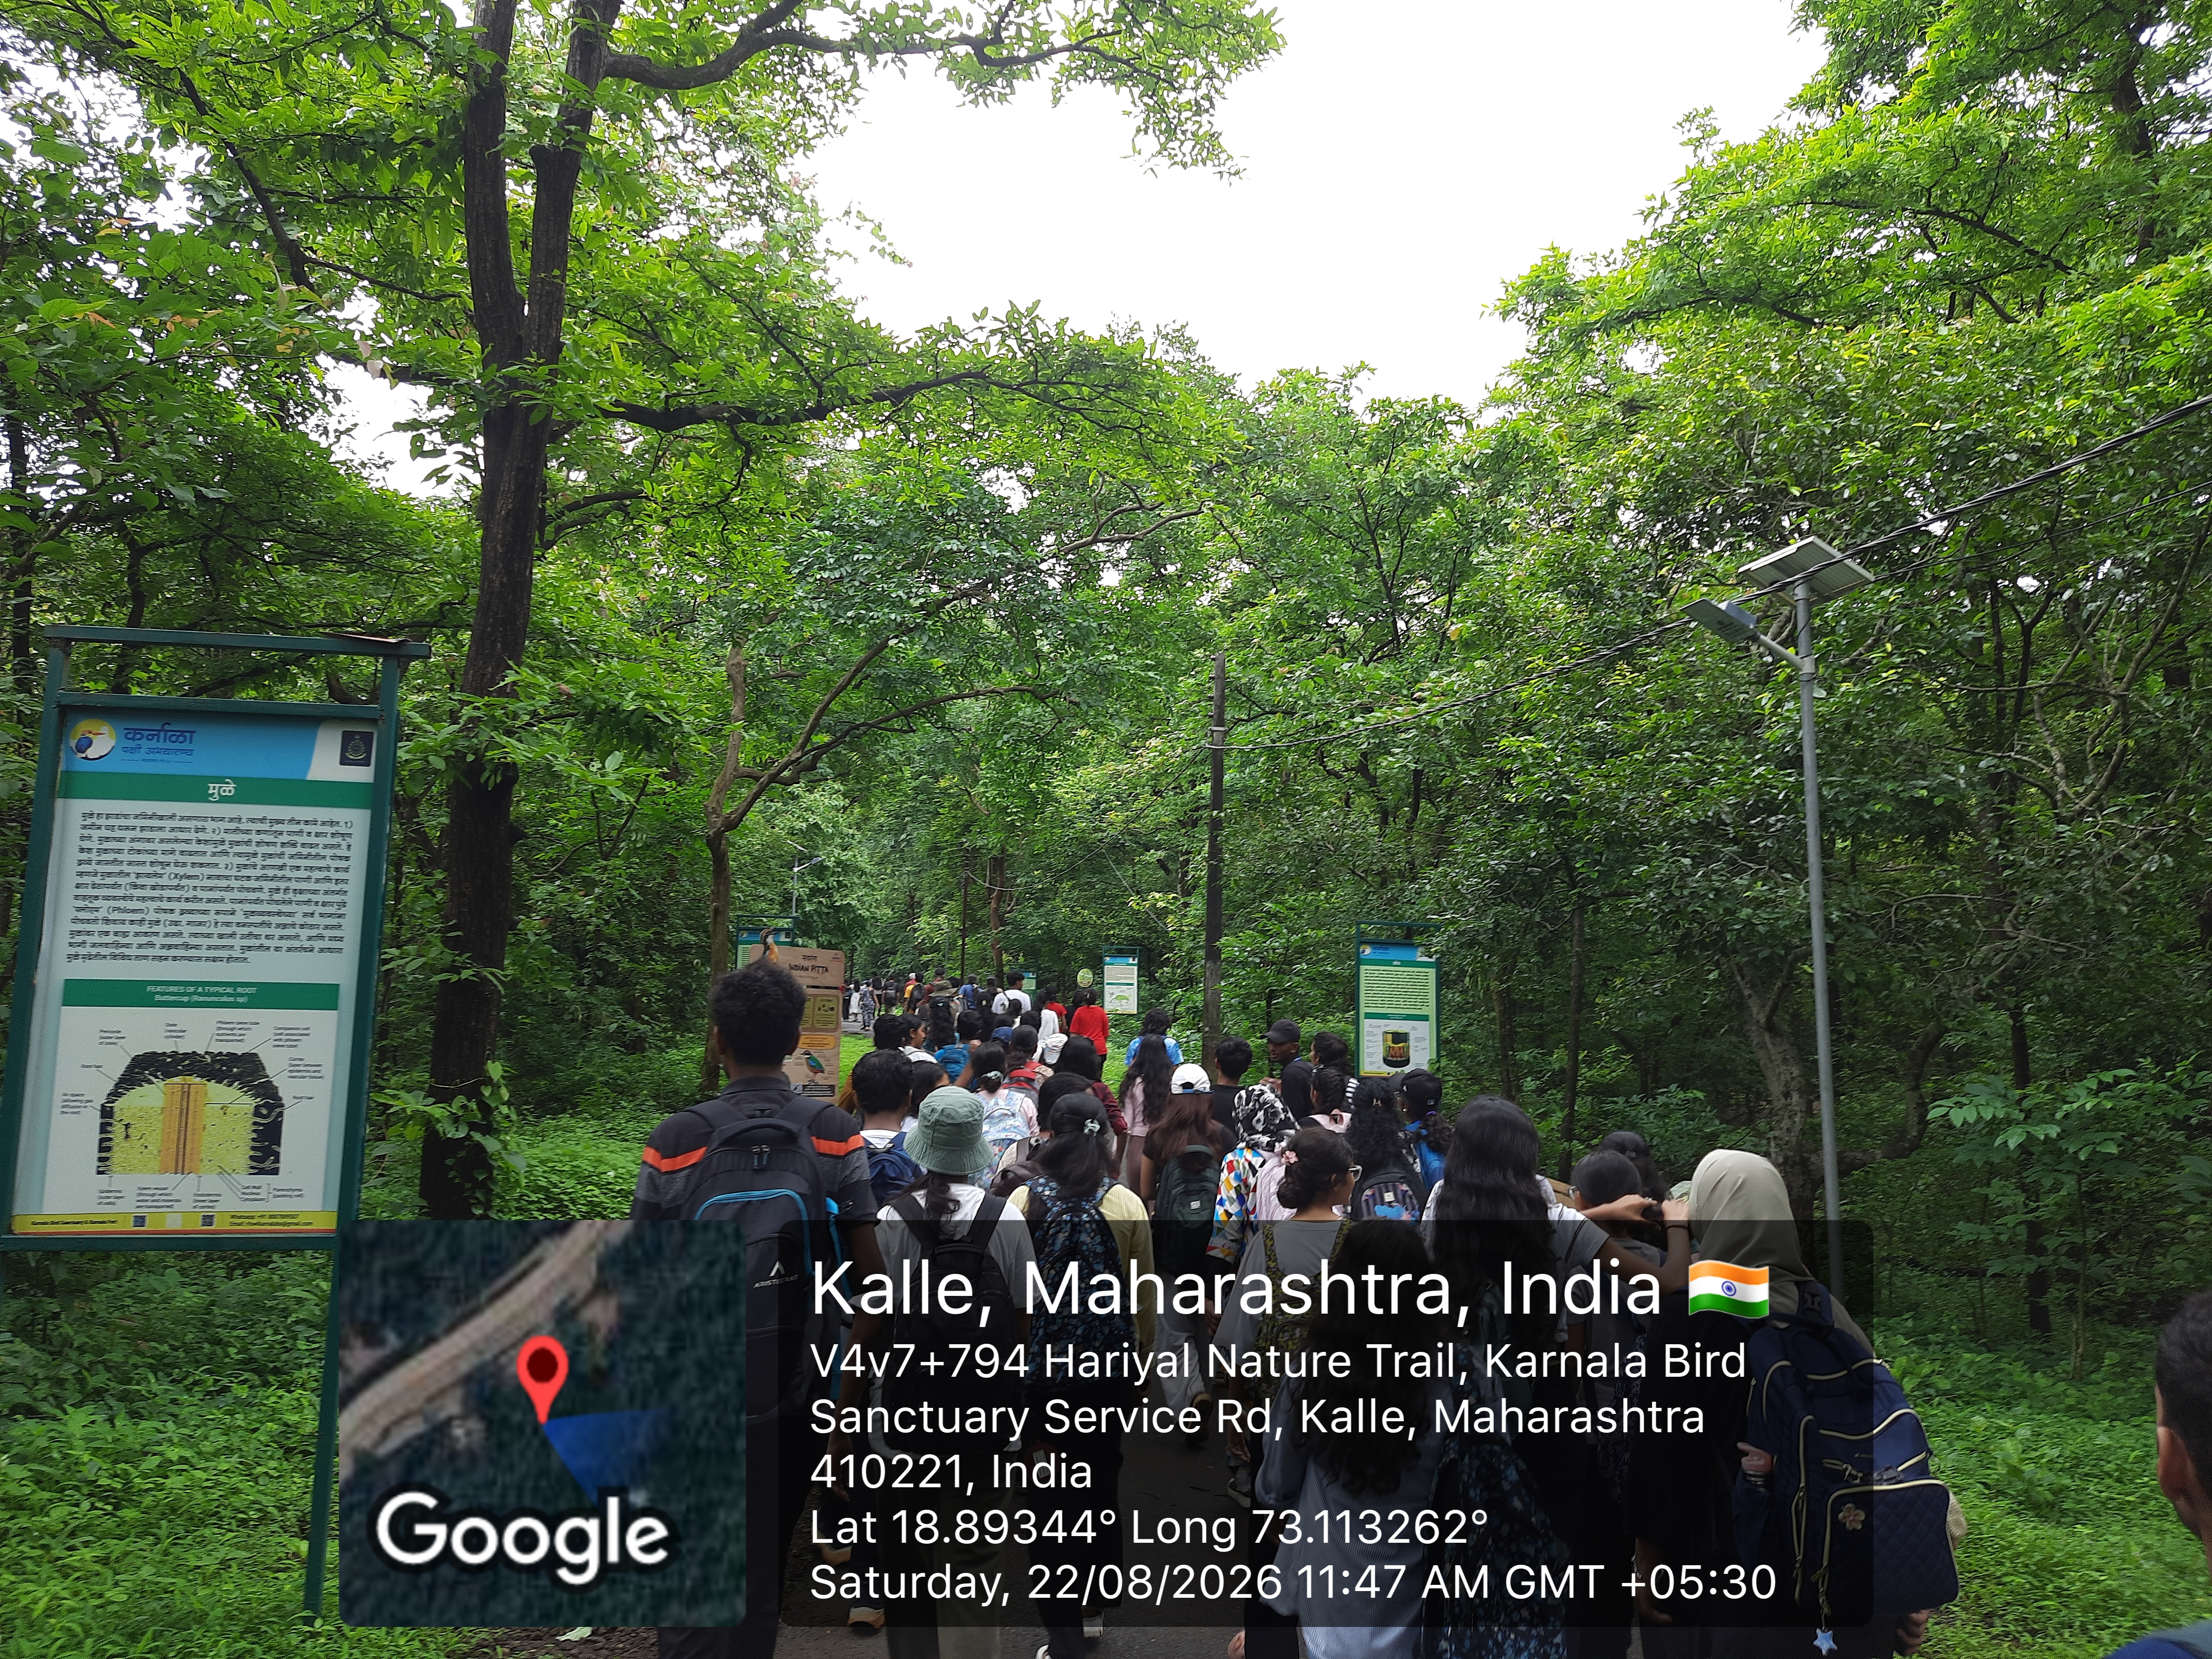
\includegraphics[width=0.7\textwidth]{route_photo2.jpg}
			
			\vspace*{1cm}
			
			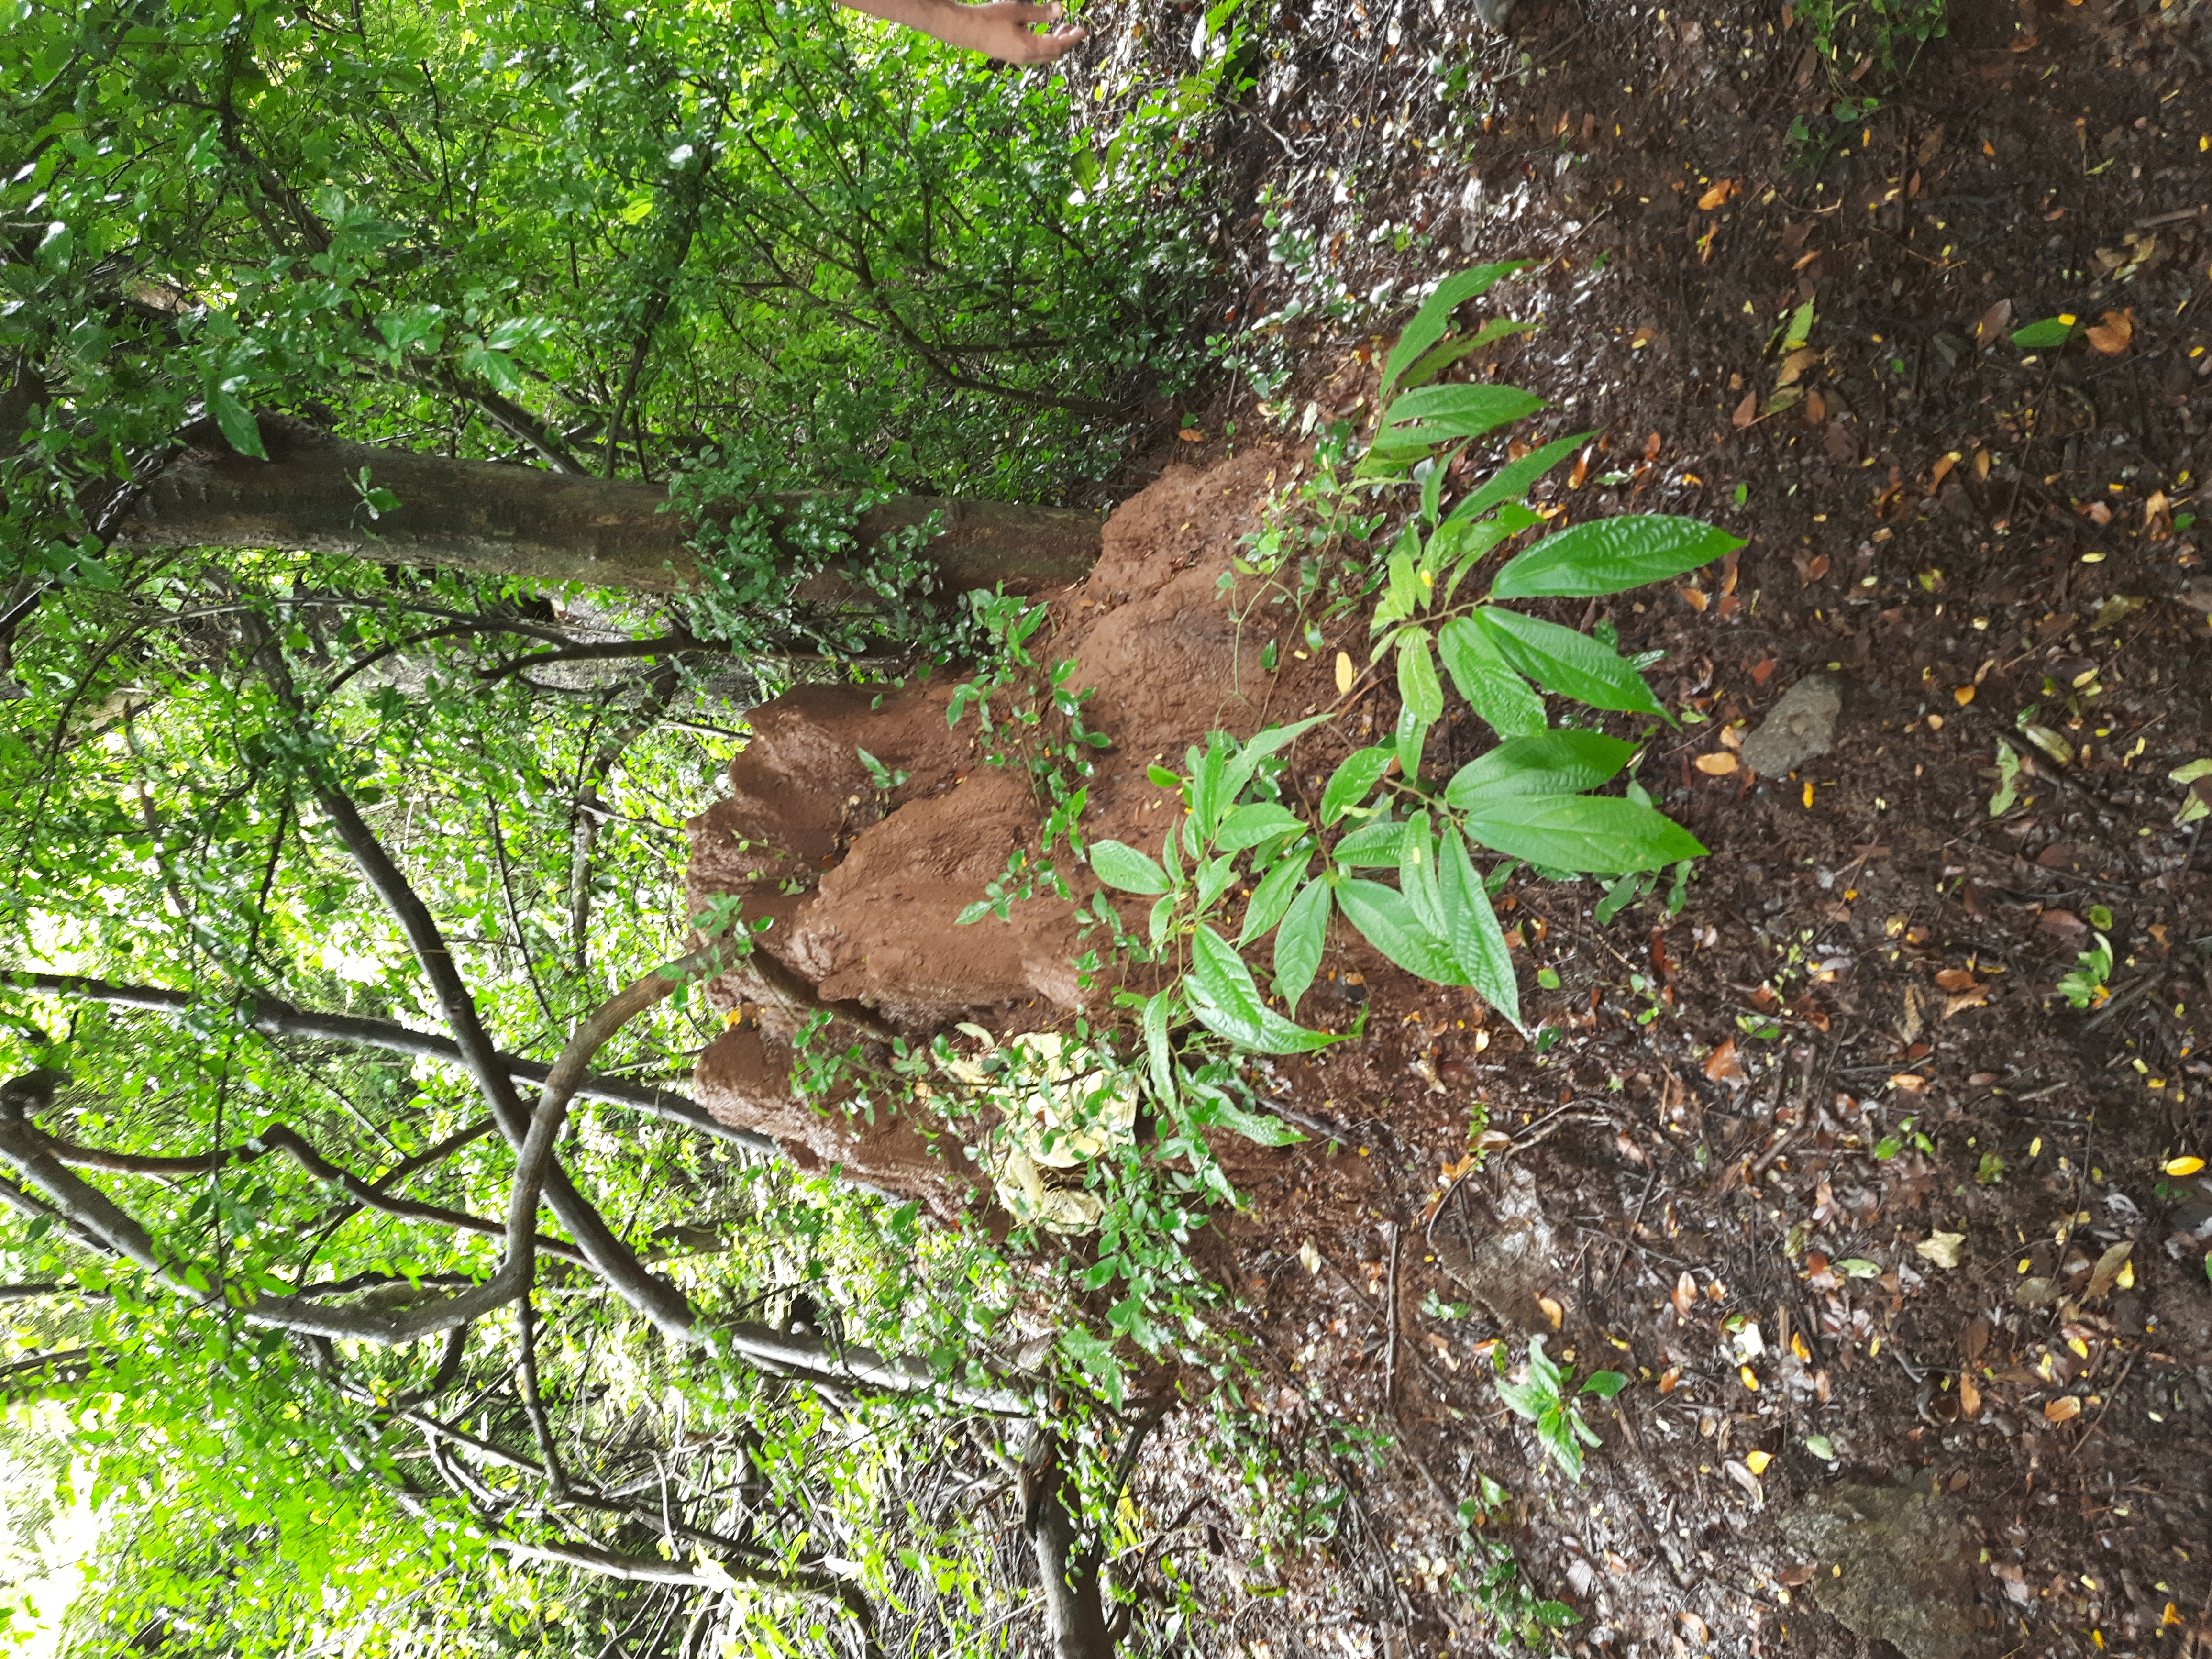
\includegraphics[height=0.6\textwidth, angle=-90]{red_ant_hill.jpg}
			\captionof{figure}{\label{fig:ant_hill}Red ant hill.}
		\end{center}
		
		A few feet from the gate, the team first spotted a red ant hill, visible in image~\ref{fig:ant_hill}.\\
		
		On the walls of an adjoining enclosure, we spotted \bfnt{\ifnt{Adiantum}}, a.k.a. Maidenhair fern. Under the old classification system, these are pteridophytes, though pteridophyta is no longer a valid taxon. As per the modern classification, we have Embryophyta\ \textrightarrow\ Tracheophyta, which further subdivides into two groups:%
%		
		\begin{enumerate}
			
			\item Lycopodiophyta; and
			
			\item Euphyllophyta, which further splits into:%
%			
			\begin{enumerate}[label={(\alph*)}]
				
				\item Polypodiophyta, under which \ifnt{Adiantum} comes, and
				
				\item Spermatophyta, which includes all seed plants.
				
			\end{enumerate}
			
		\end{enumerate}
		
		Following PPG~I (2016), the exact classification goes as follows:\\
		
		Eukarya\ \ \textrightarrow\ \ Archaeplastida\ \ \textrightarrow\ \ Viridiplantae\ \ \textrightarrow\ \ Streptophyta\ \ \textrightarrow\ \ Embryophyta\ \ \textrightarrow\ \ Tracheophyta\ \ \textrightarrow\ \ Euphyllophyta\ \ \textrightarrow\ \ Polypodiophyta\ \ \textrightarrow\ \ Polypodiidae\ \ \textrightarrow\ \ Polypodiales\ \ \textrightarrow\ \ Pteridaceae\ \ \textrightarrow\ \ Vittarioideae\ \ \textrightarrow\ \ \ifnt{Adiantum sp.}
		
		\begin{center}
			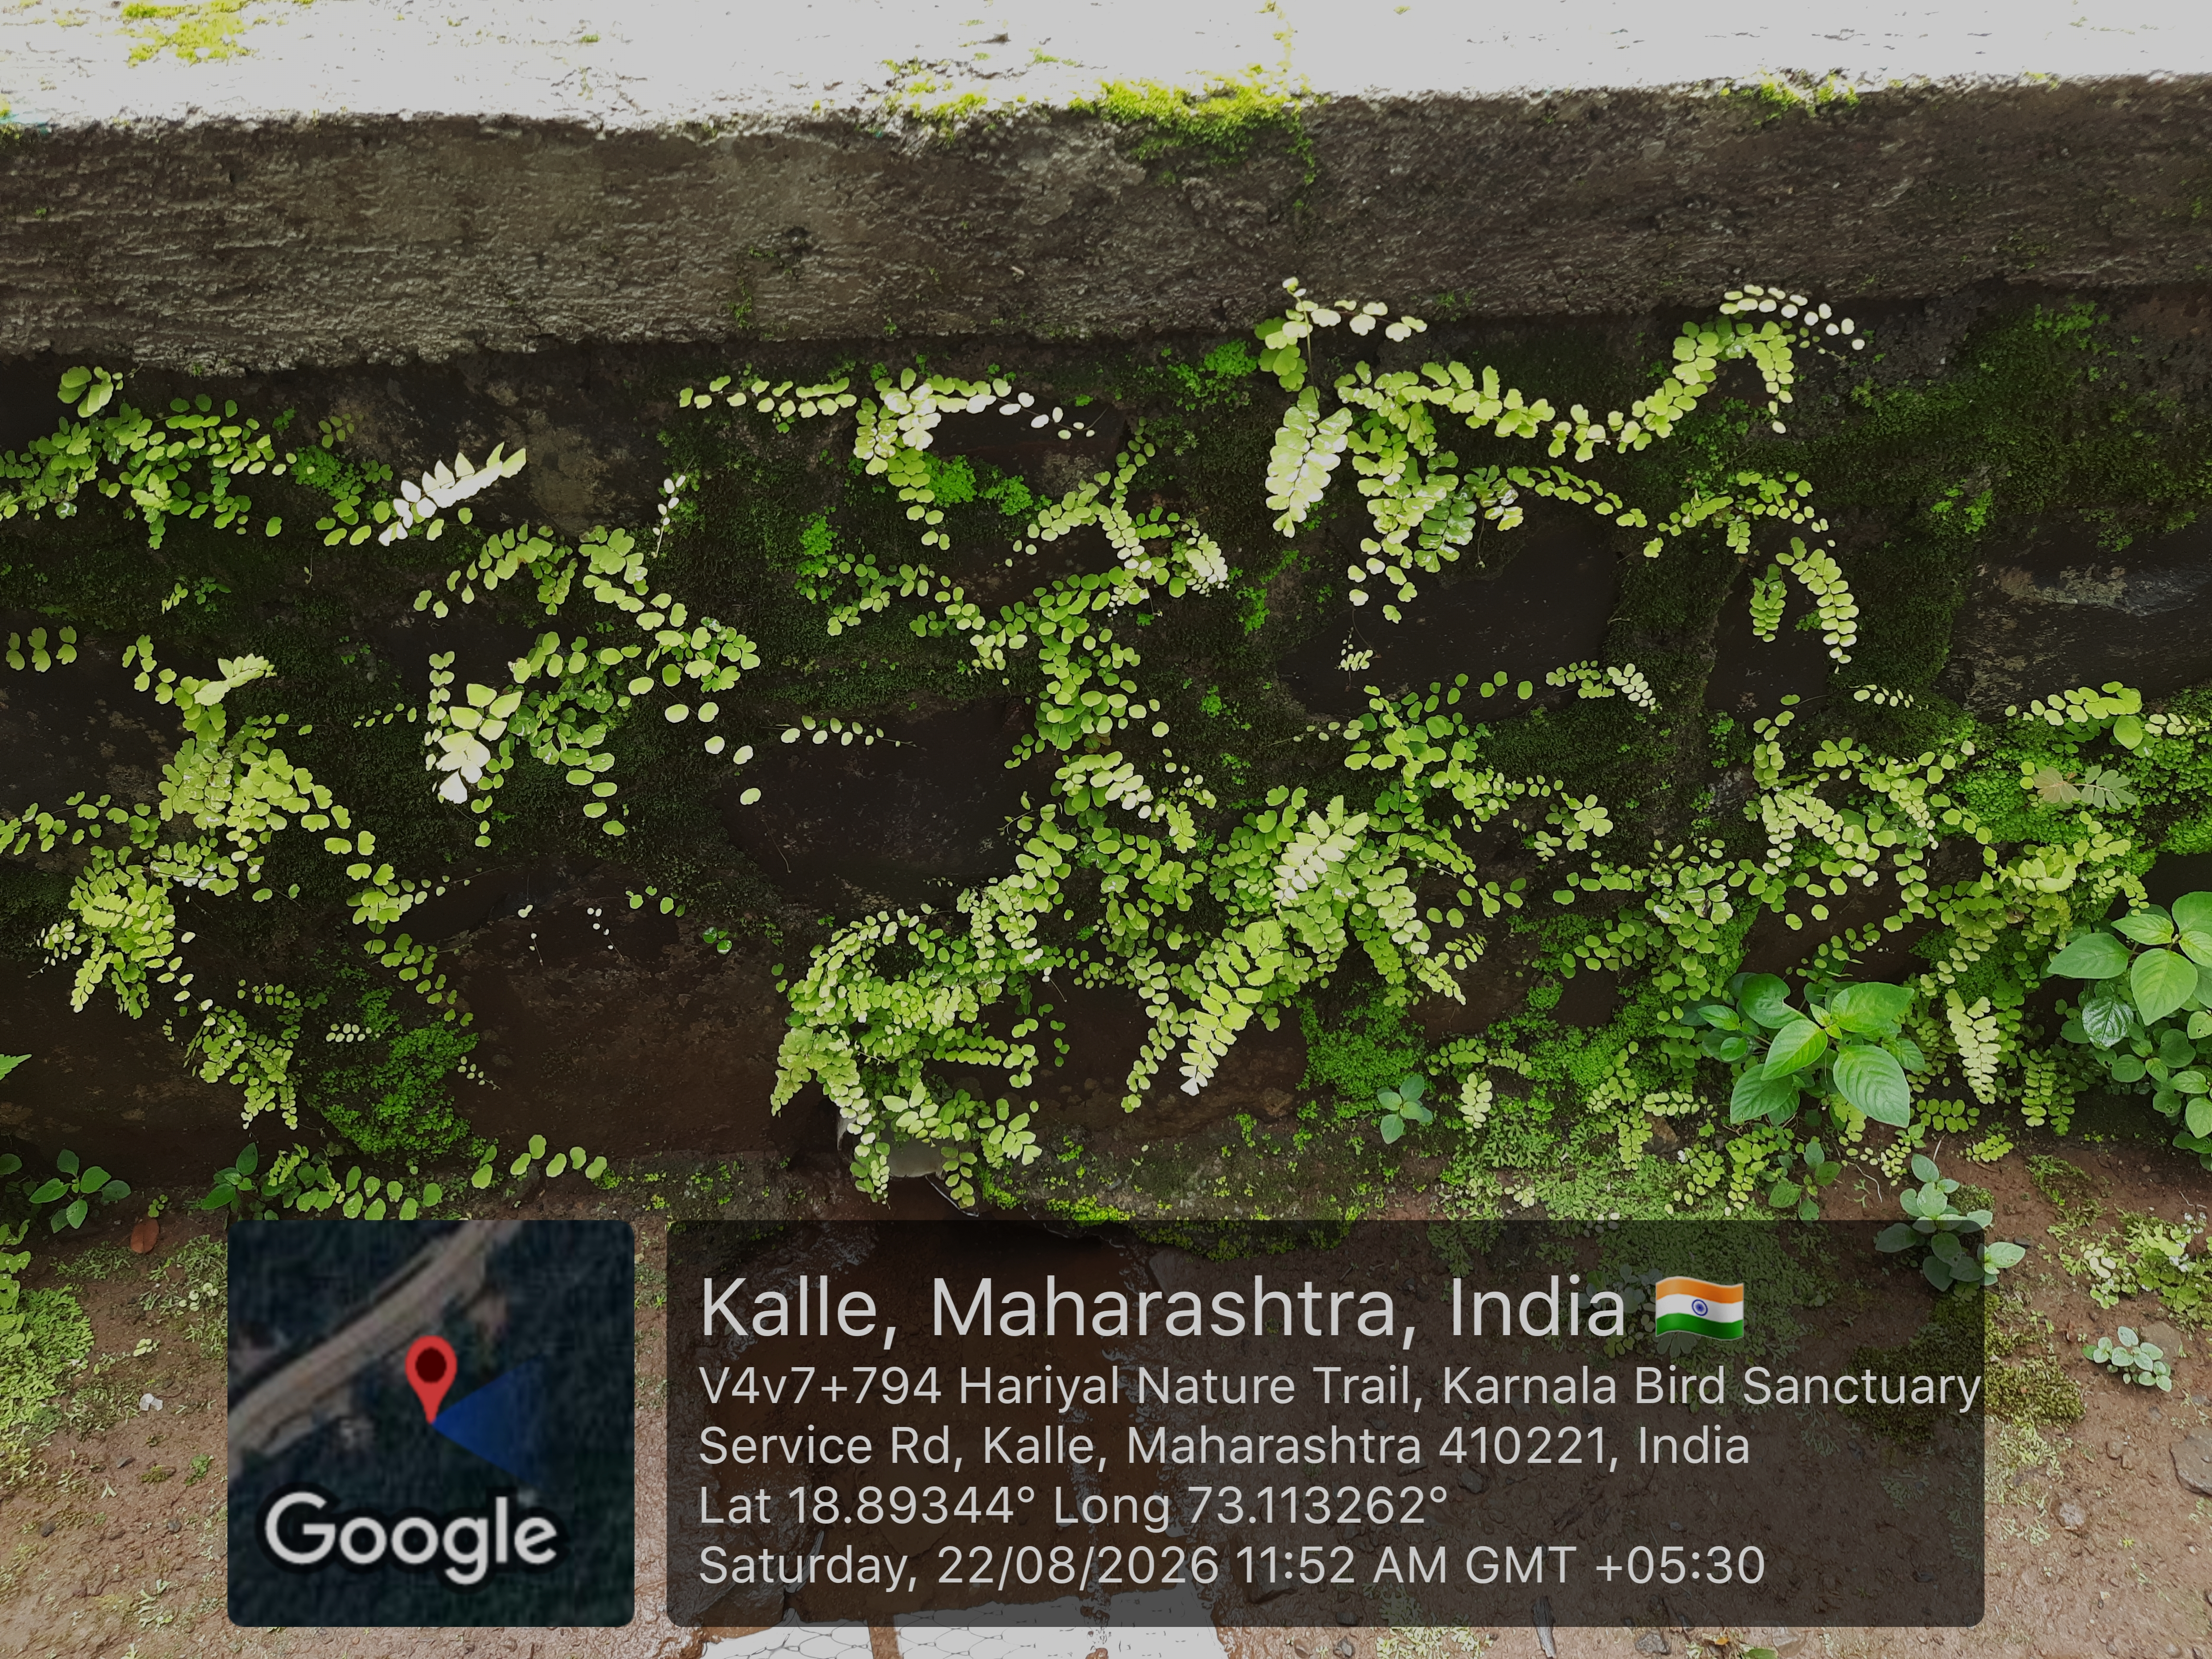
\includegraphics[width=0.8\textwidth]{fern_moss.jpg}
			\captionof{figure}{\ifnt{Adiantum sp.}, along with moss on the wall.}
		\end{center}
		
		A little rock nearby had crustose lichen growing on it, as seen in image~\ref{fig:lichen}. Before we proceed, lichens deserve a word or two. A lichen is not a taxon of its own, because it is not a single type of organism. A lichen is a symbiotic phenotype of an alga and a fungus. The fungus helps in deriving nutrition from dead and decaying matter, while the alga photosynthesises from whatever sunlight is available. Under botanical code, the name of a lichen is derived from its fungal partner. Lecanoromycetes is a large class of lichens, though there are more. There are even lichens where the the other partner is not even an eukaryote.\\
		
		Based on growth forms, lichens can be divided among the following categories:%
%		
		\begin{enumerate}
			
			\item \bfnt{Crustose:} thallus fused to the substrate with no lower cortex, cannot be removed intact. E.g. \ifnt{Lecanora}, \ifnt{Graphis}, \ifnt{Rhizocarpon}.
			
			\item \bfnt{Foliose:} leaf-like and dorsiventral, with upper and lower cortex, attached by rhizines. E.g. \ifnt{Parmelia}, \ifnt{Xanthoria}, and \ifnt{Peltigera}.
			
			\item \bfnt{Fruticose:} shrubby or pendulous, radially symmetrical in section.  E.g. \ifnt{Usnea}, \ifnt{Cladonia}, \ifnt{Ramalina}.
			
			\item \bfnt{Squamulose:} small overlapping scales or squamules, loosely attached at one edge, intermediate between crustose and foliose. E.g. \ifnt{Cladonia} basal thallus, \ifnt{Psora}.
			
			\item \bfnt{Gelatinous:} homoiomerous, always with a cyanobacterial photobiont, usually \ifnt{Nostoc}. Dry and brittle when dehydrated, swelling into a dark jelly when wet. E.g.  \ifnt{Collema}, \ifnt{Leptogium}.
			
			\item \bfnt{Filamentous:} fungal hyphae wrapped around filaments of the photobiont, producing a hair-like or felty thallus. \ifnt{Ephebe}, \ifnt{Cystocoleus}, \ifnt{Racodium}.
			
			\item \bfnt{Byssoid:} wispy, like teased wool.
			
			\item \bfnt{Foliicolous:} growing on living leaves, common in tropical humid forests including the Western Ghats.
			
		\end{enumerate}
		
		\begin{center}
			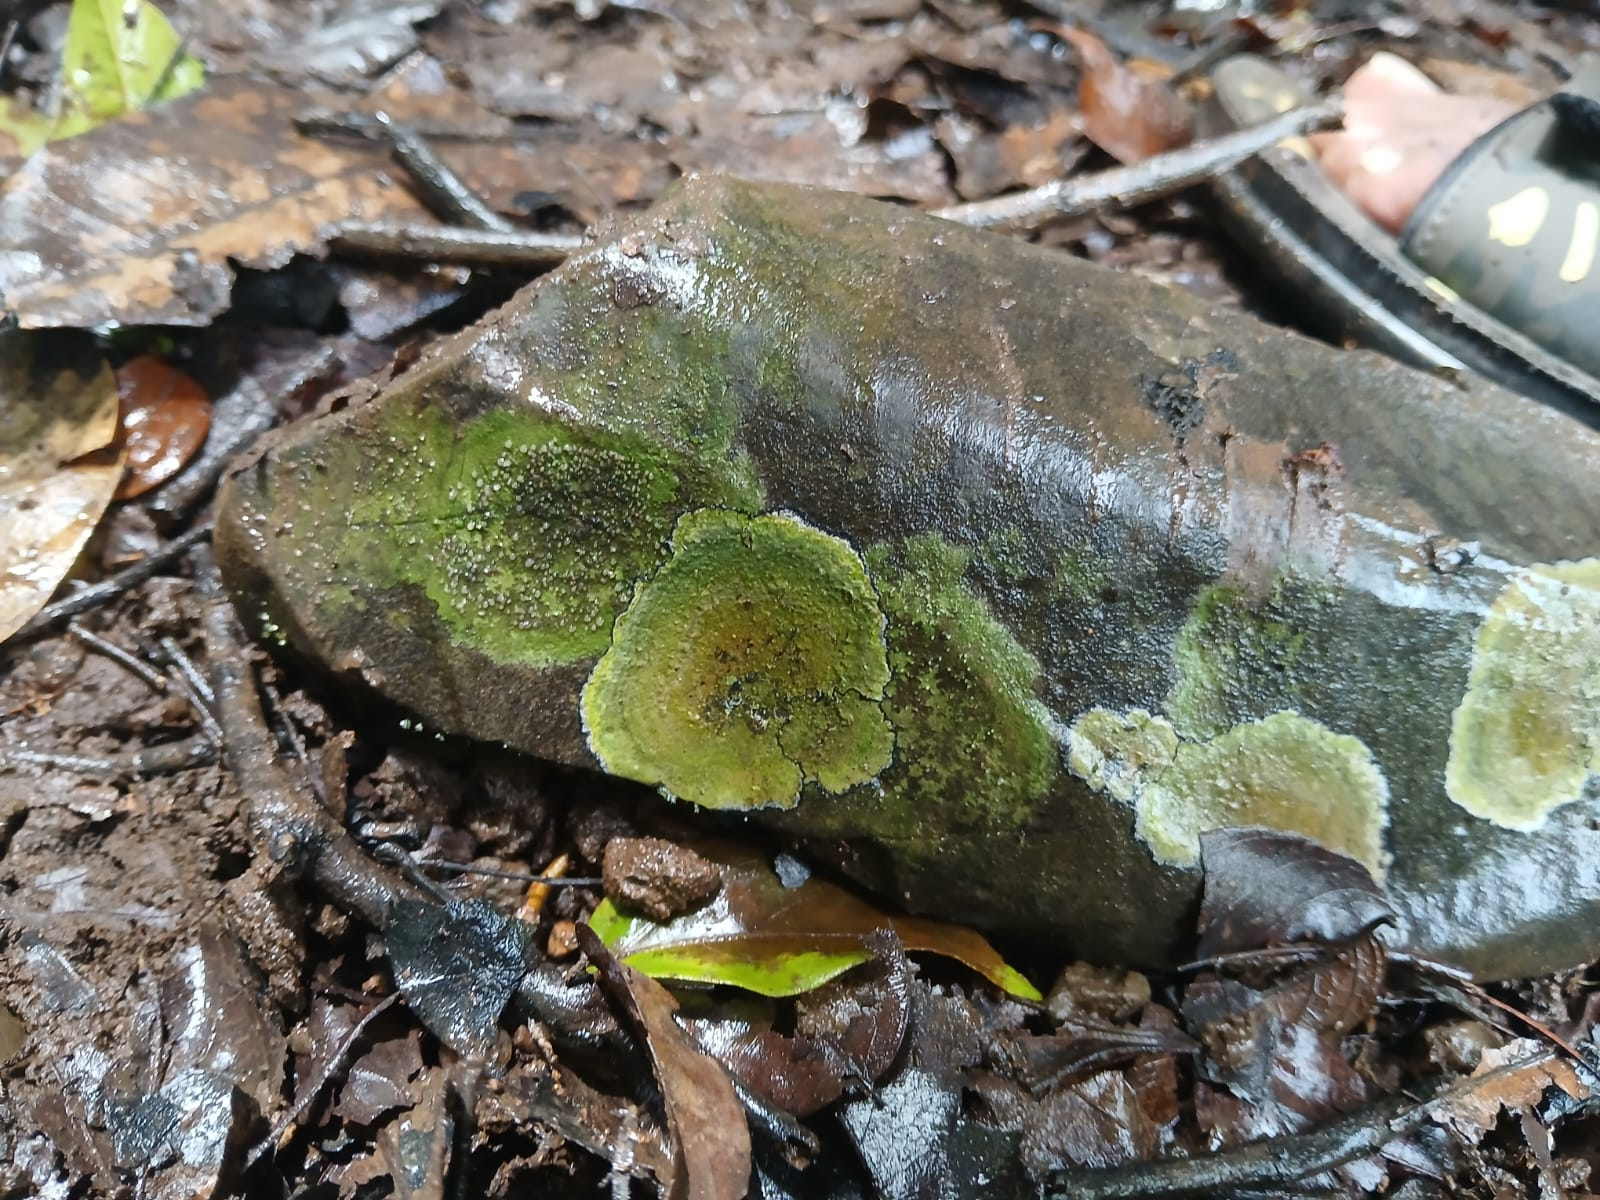
\includegraphics[width=0.6\textwidth]{crustose.jpg}
			\captionof{figure}{\label{fig:lichen}Crustose lichen on a tiny rock.}
		\end{center}
		
		\clearpage
		
		\begin{center}
			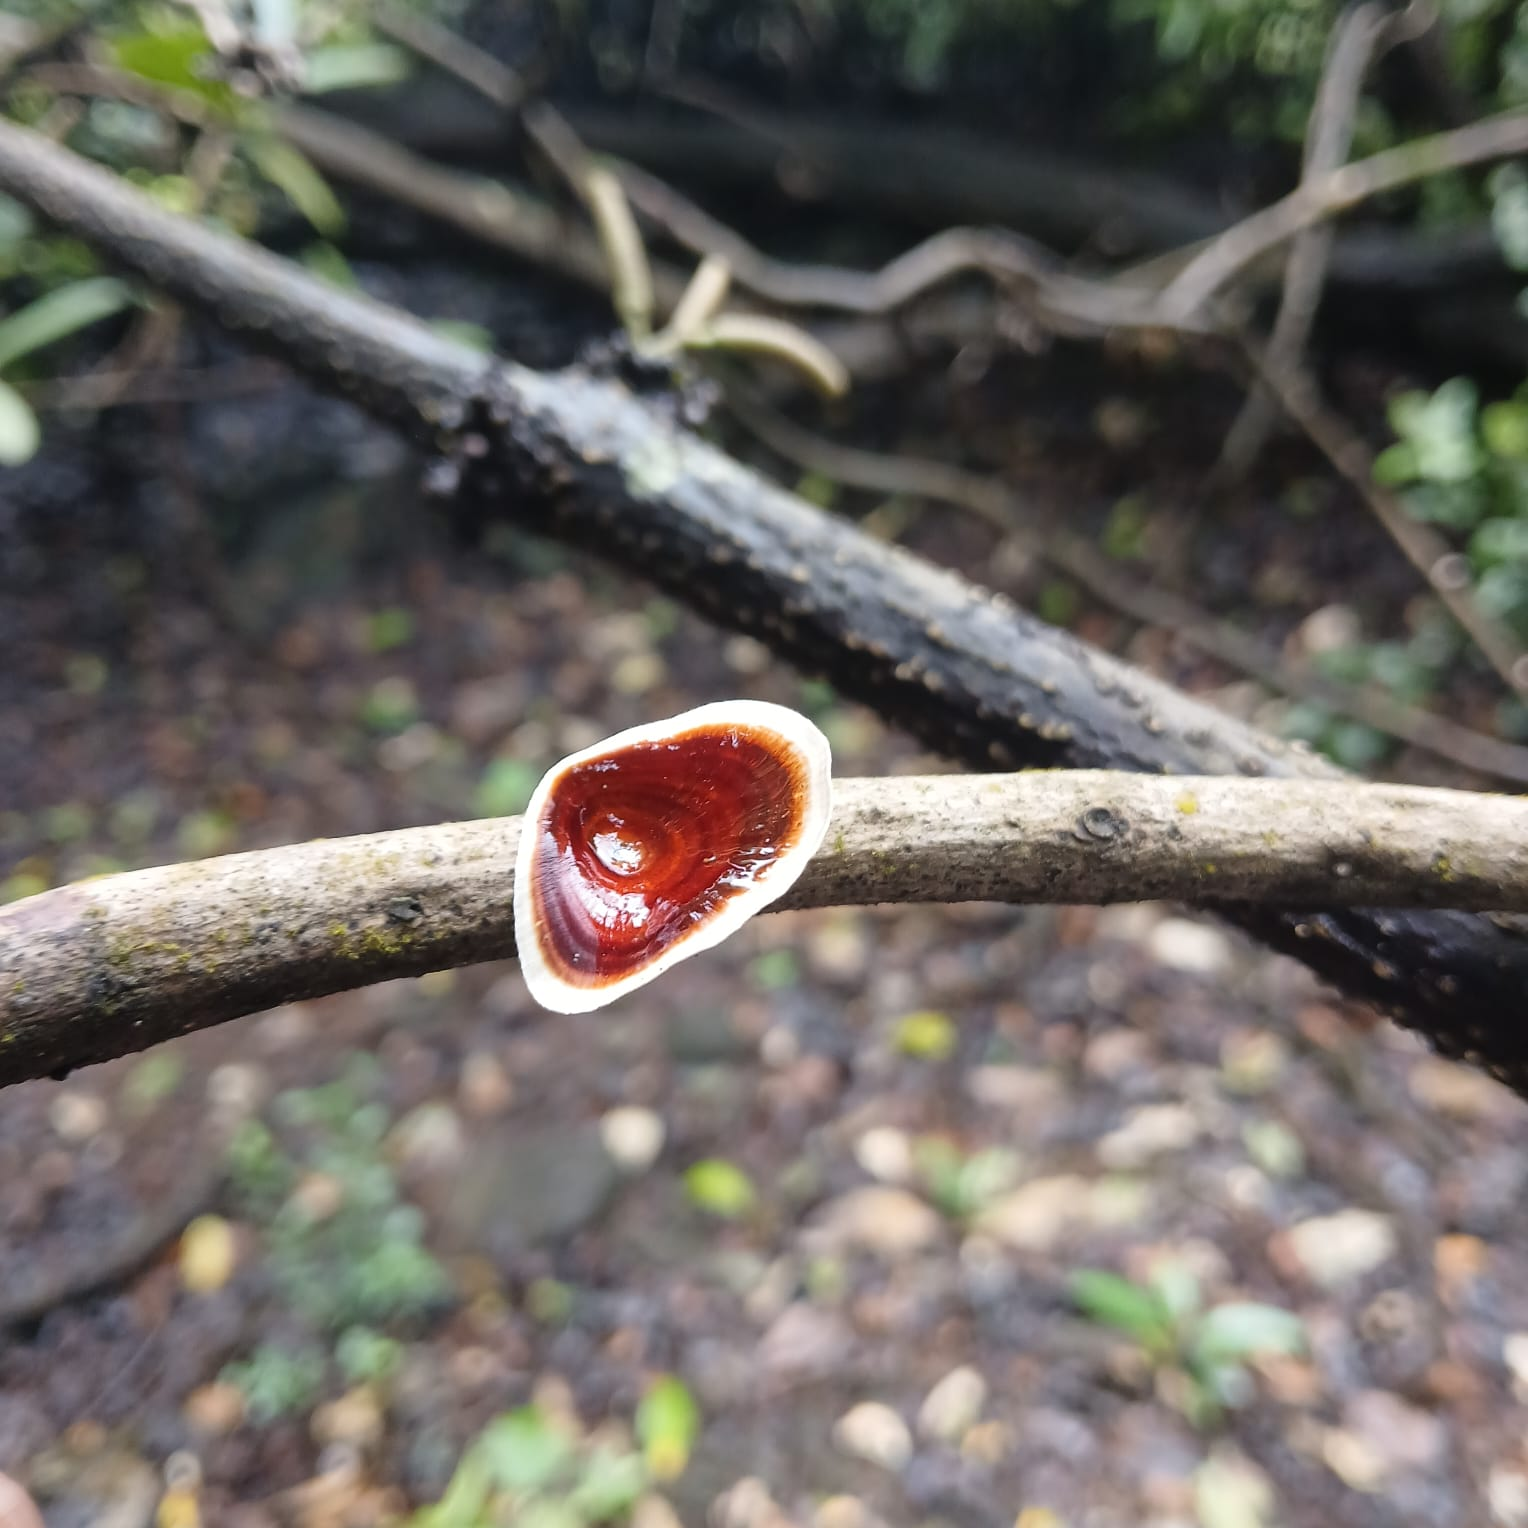
\includegraphics[width=0.5\textwidth]{bracket_fungus.jpg}
			\captionof{figure}{Bracket fungus}
			
			\vfill
			
			\includegraphics[width=0.8\textwidth,angle=-90]{wood_rotting_fungus.jpg}
			\captionof{figure}{Wood rotting fungus}
		\end{center}
		
		\clearpage
		
		\begin{center}
			\vspace*{1cm}
			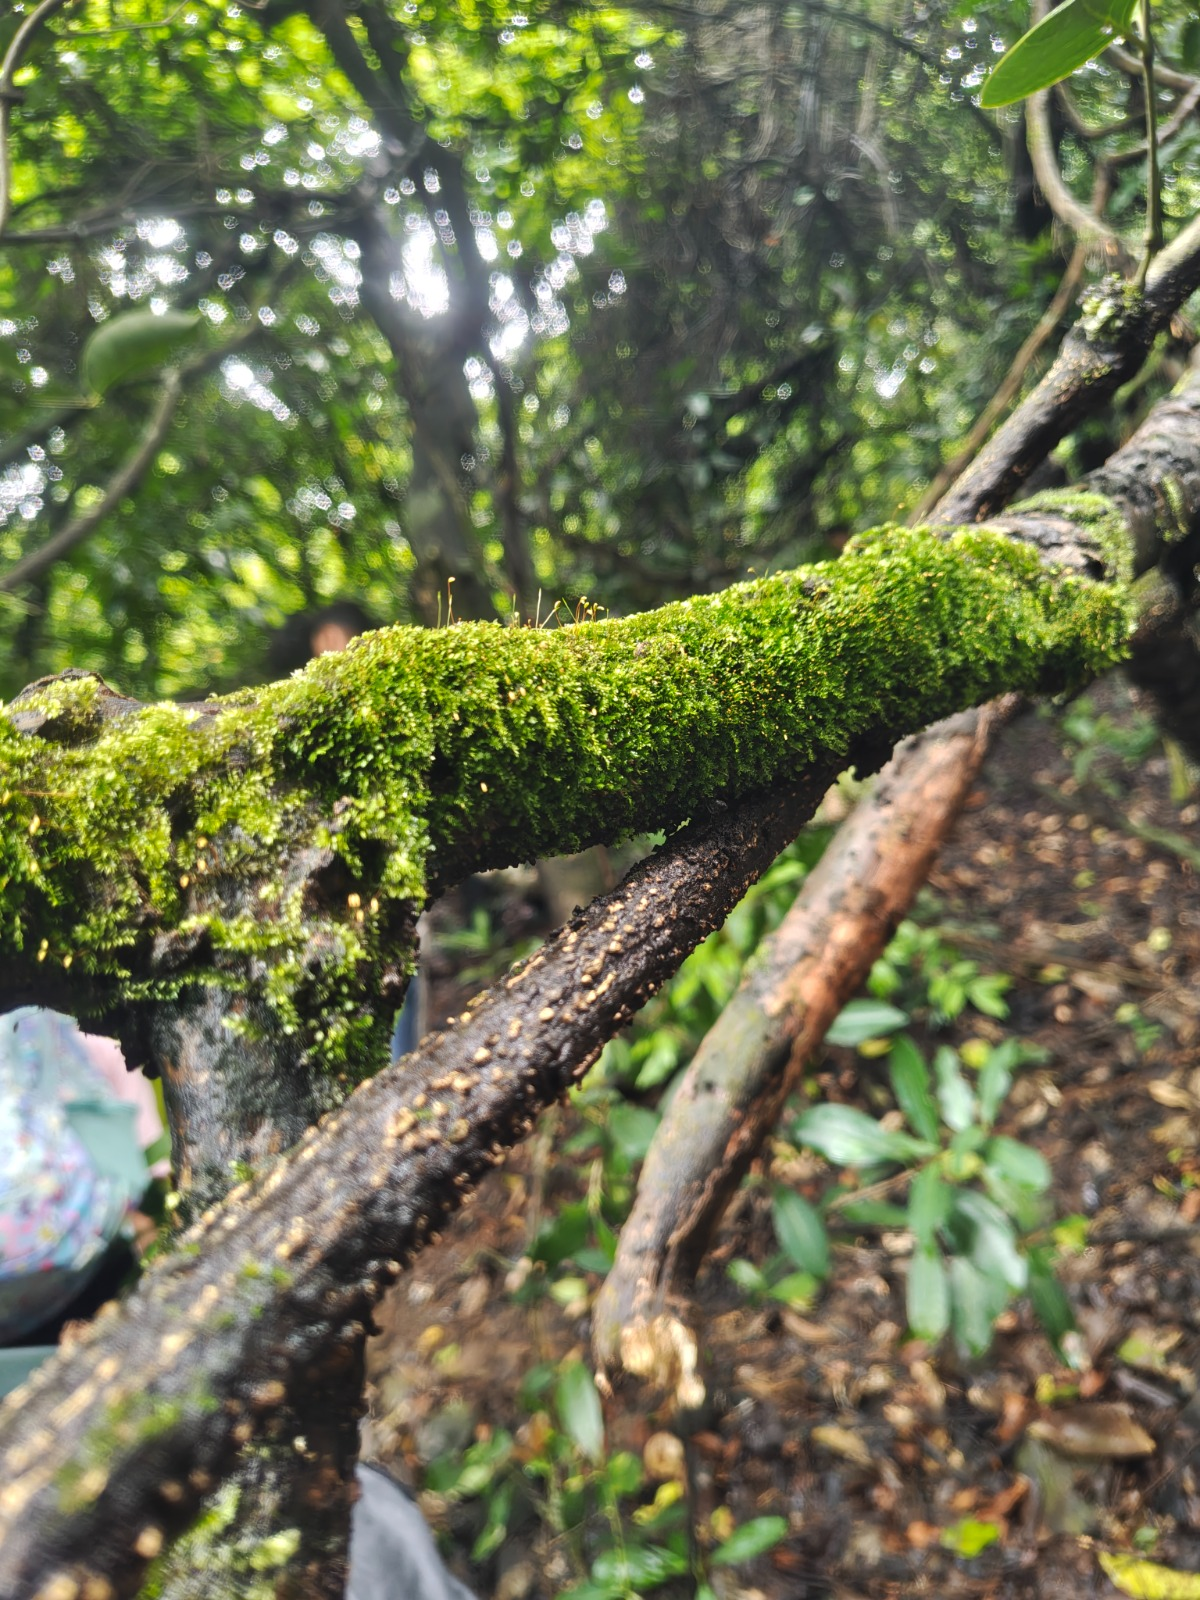
\includegraphics[width=0.7\textwidth]{moss.jpg}
			\captionof{figure}[Moss growing on a tree]{Moss growing on a tree. Scattered across the mat are slender pale setae, each roughly a centimetre or two long, carrying a small capsule at the tip. Those are sporophytes, so this colony is reproducing sexually right now, which is typical after sustained monsoon wetting. The colony is pleurocarpous --- the mat form, the branching, and the setae emerging from the sides of prostrate shoots rather than from erect tips all point to pleurocarpous. Nearly all pleurocarpous mosses sit in class Bryopsida, subclass Bryidae, and the big epiphytic families in the Western Ghats are Hypnaceae, Brachytheciaceae, Neckeraceae, Sematophyllaceae and Pterobryaceae.}
		\end{center}
		
		\clearpage
		
		\begin{center}
			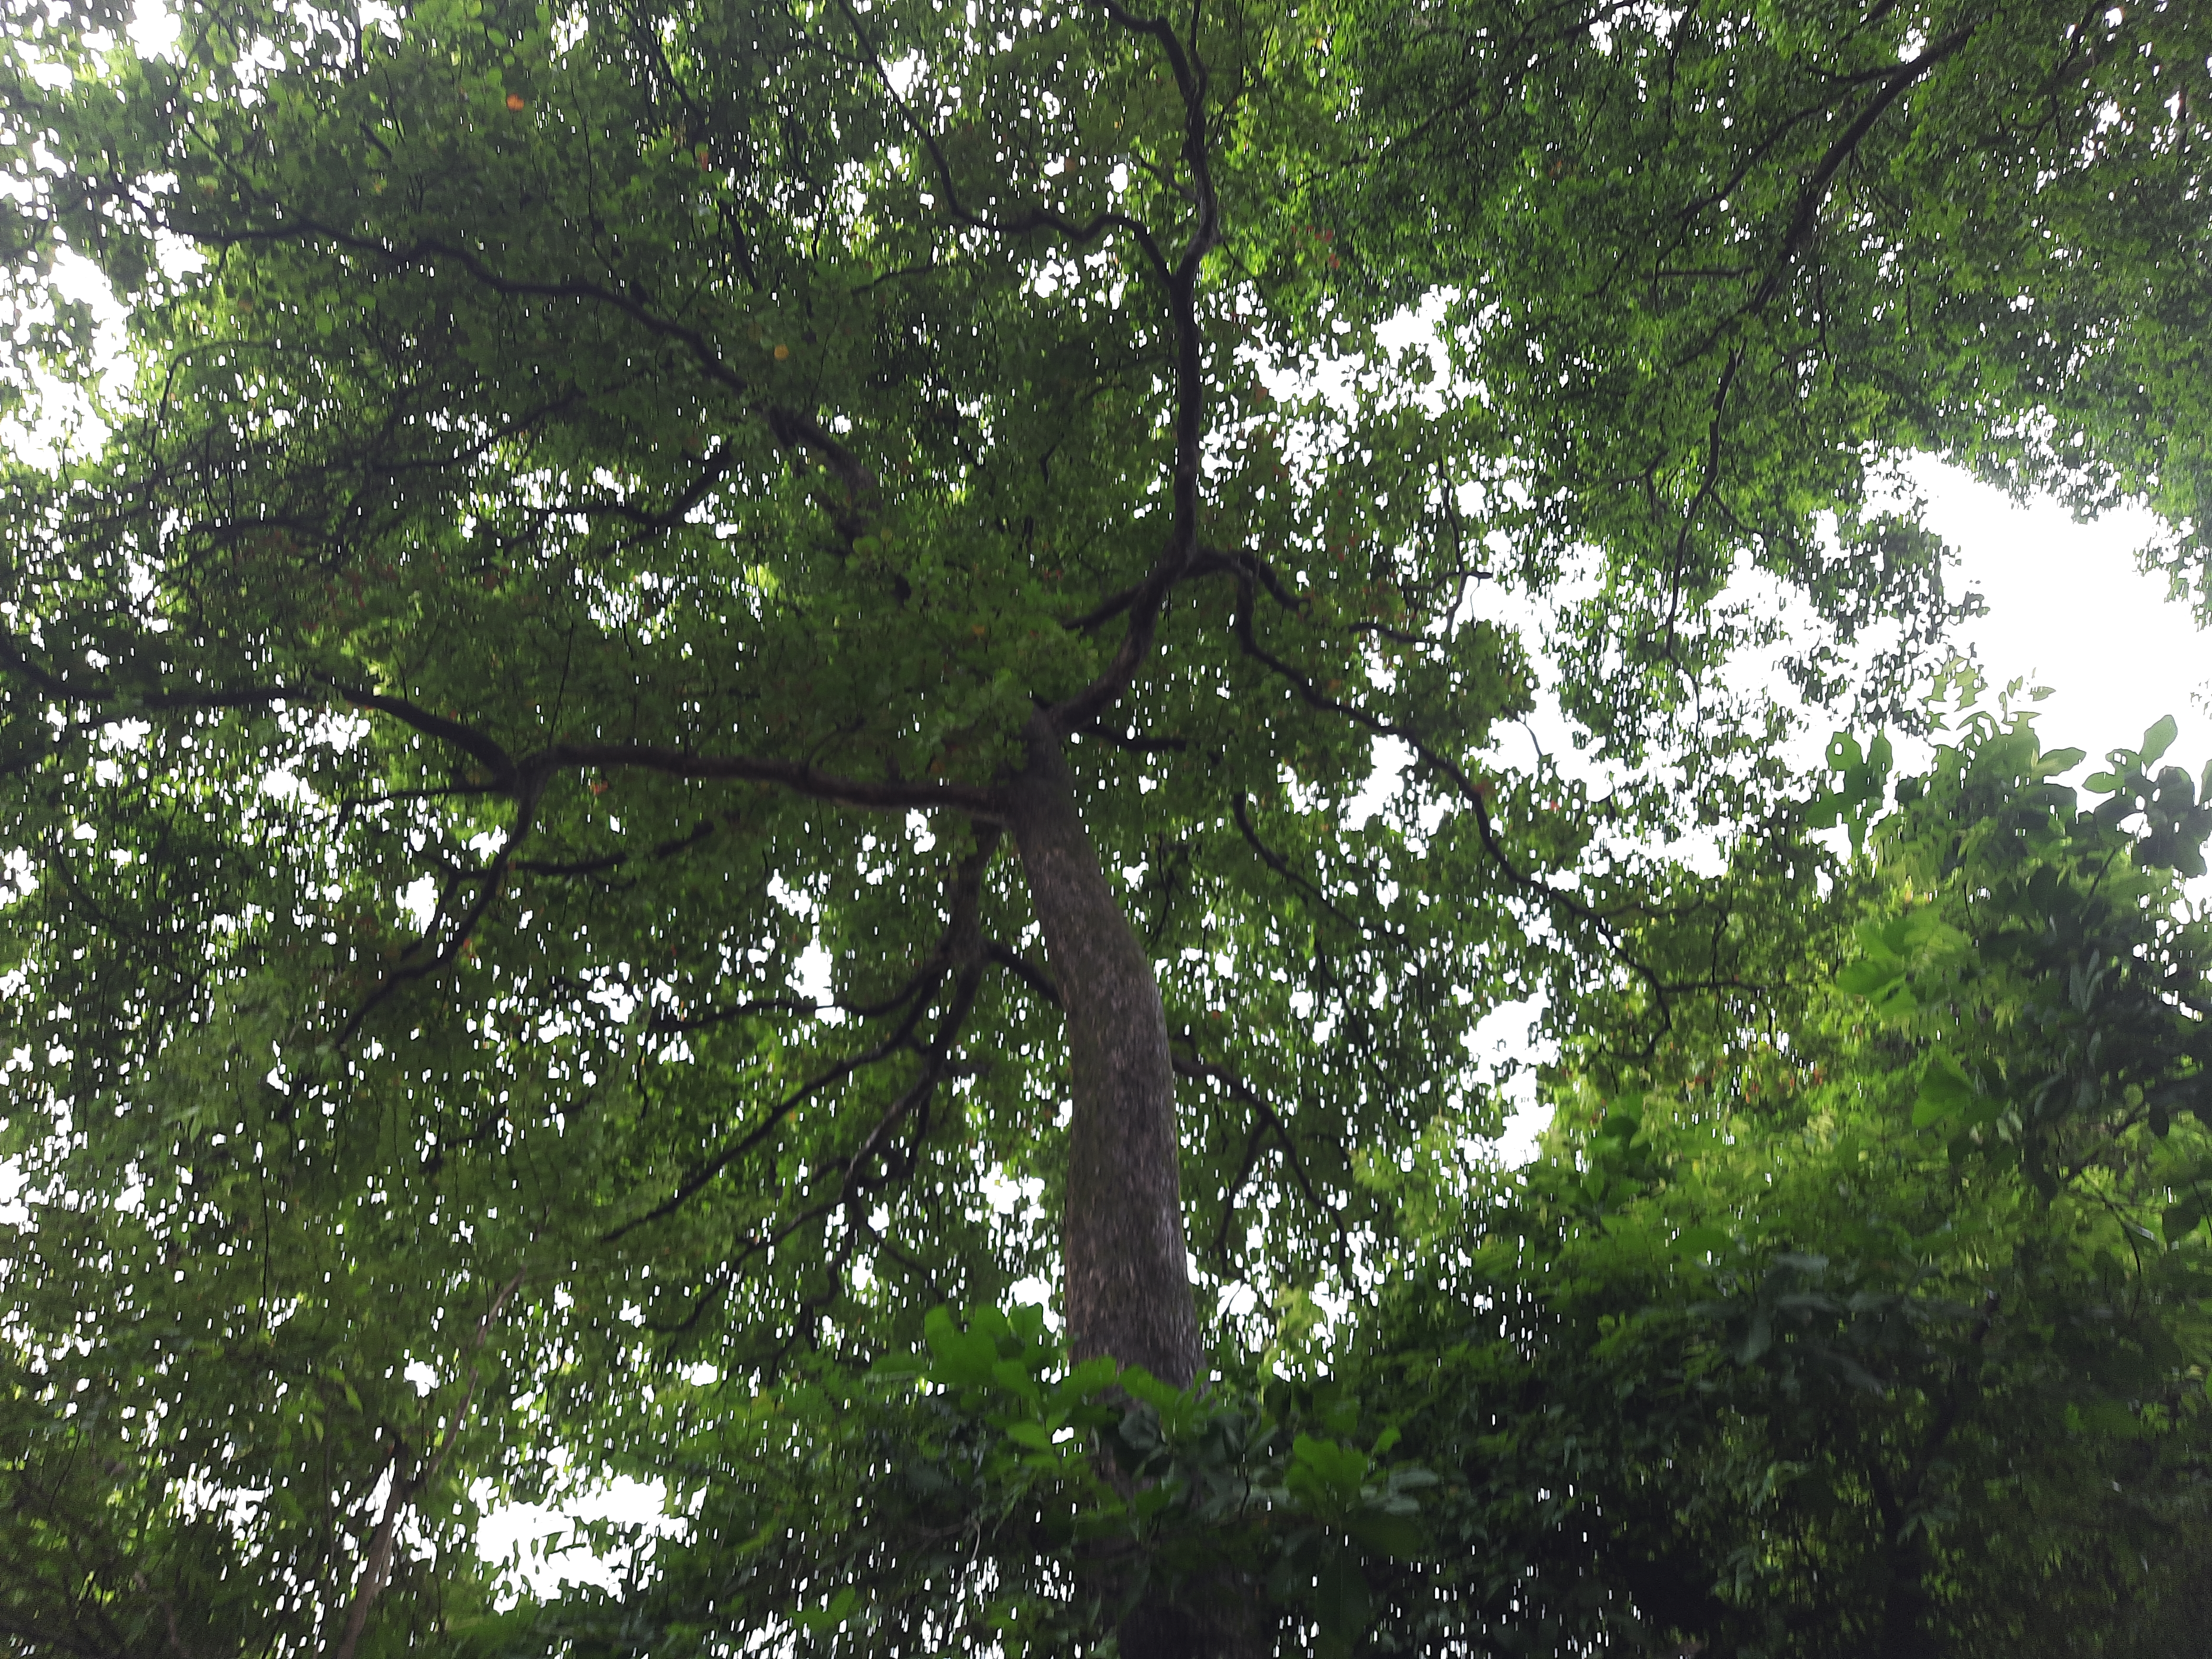
\includegraphics[width=0.8\textwidth]{canopy1.jpg}
			\vfill
			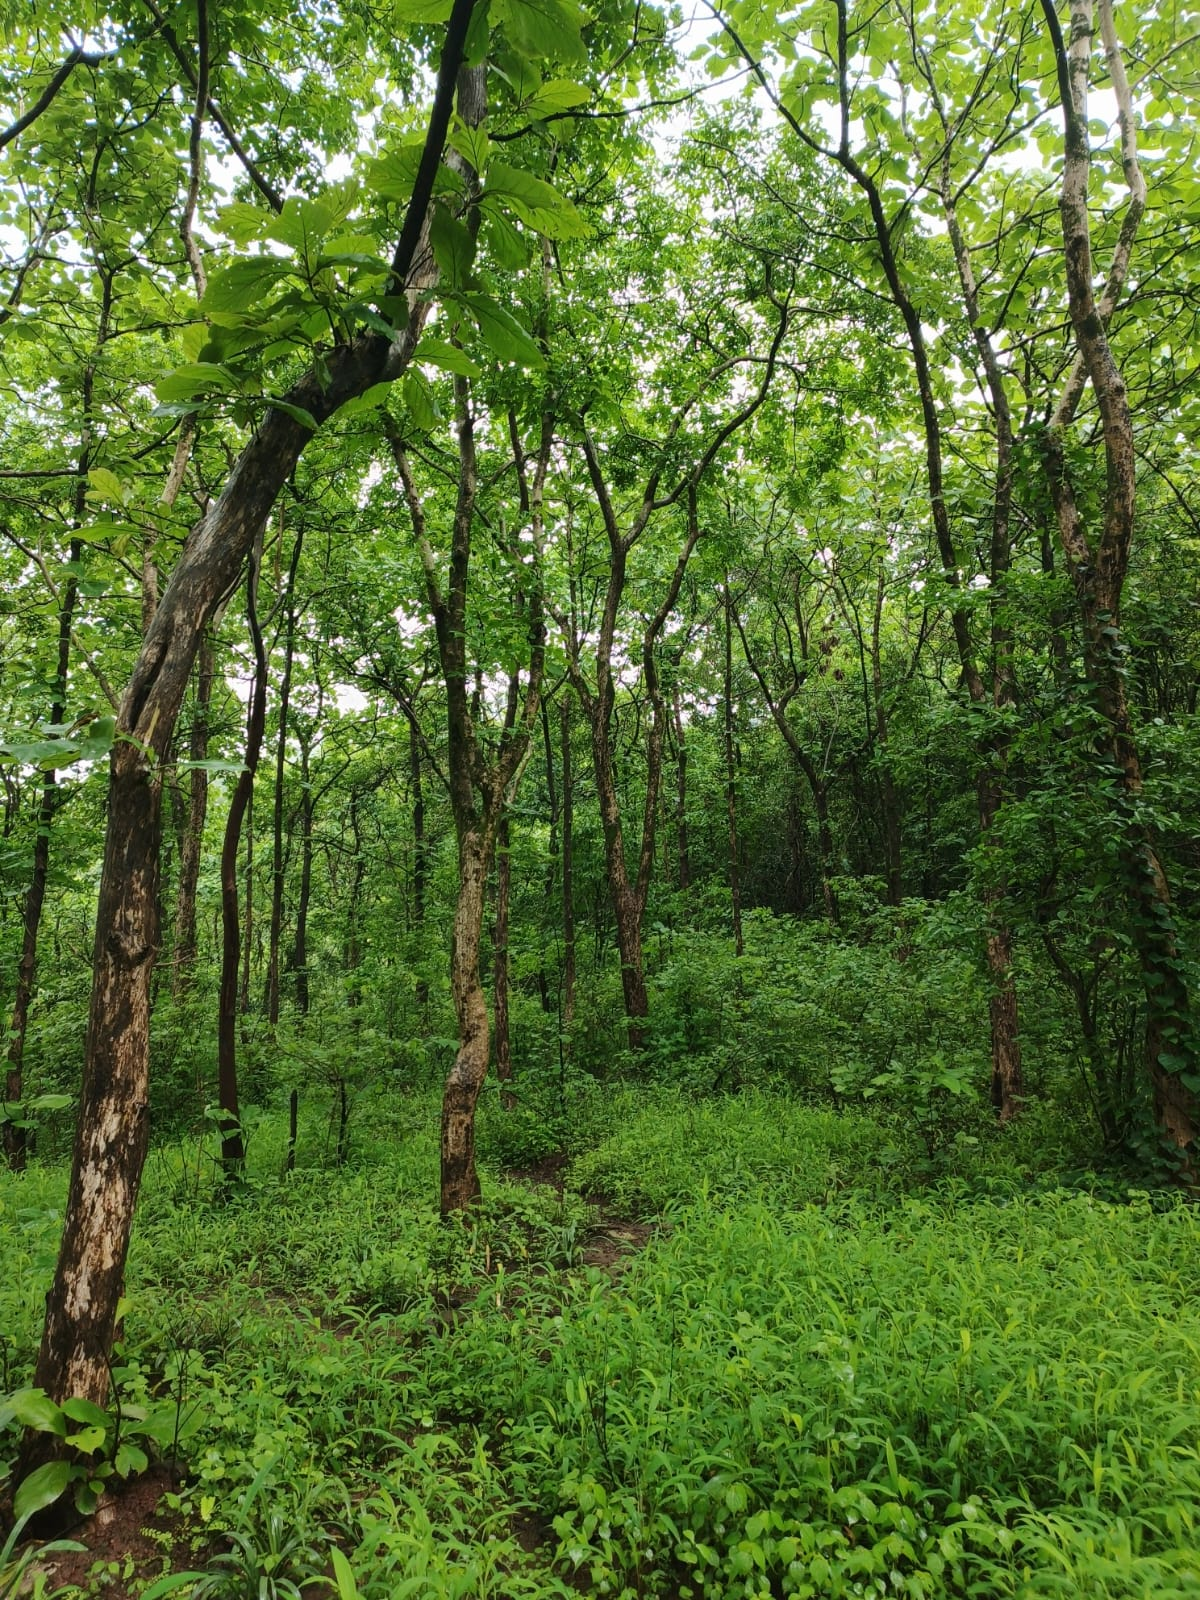
\includegraphics[width=0.55\textwidth]{canopy2.jpg}
			\captionof{figure}{Top \& bottom: Forest wilderness and canopy in the monsoon}
		\end{center}
		
		\begin{center}
			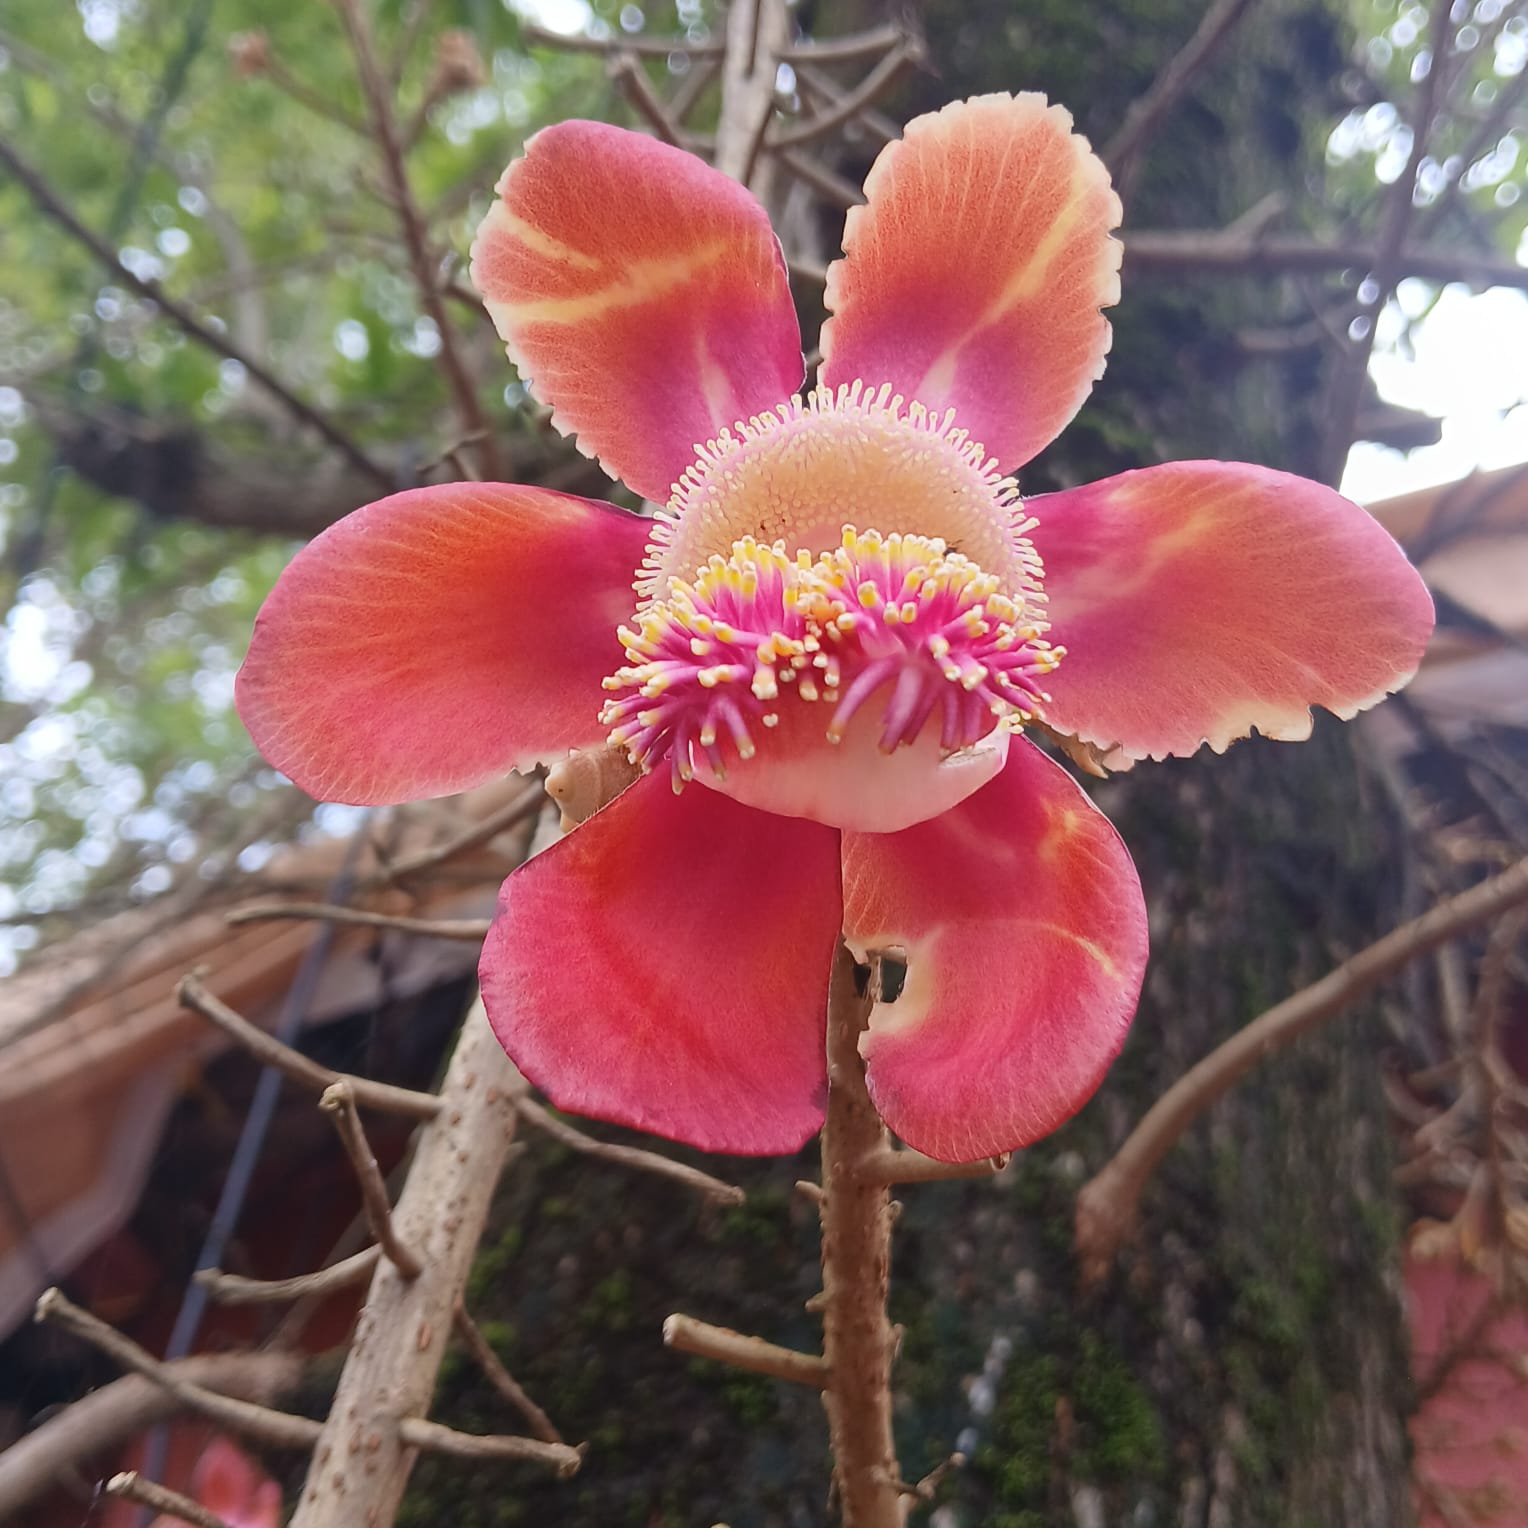
\includegraphics[width=0.6\textwidth]{Kailashpati.jpg}
			\captionof{figure}[\ifnt{Couroupita guianensis} -- Kailashpati]{\ifnt{Couroupita guianensis} -- the Kailashpati tree, a.k.a. the Kaurav Pandav flower. A small Shivling type structure seen inside the flower. Very fragrant. Fruits are known as cannon ball. Directly arises from the main trunk so called as cauliflorous.}
			
			\vspace*{1.2cm}
			
			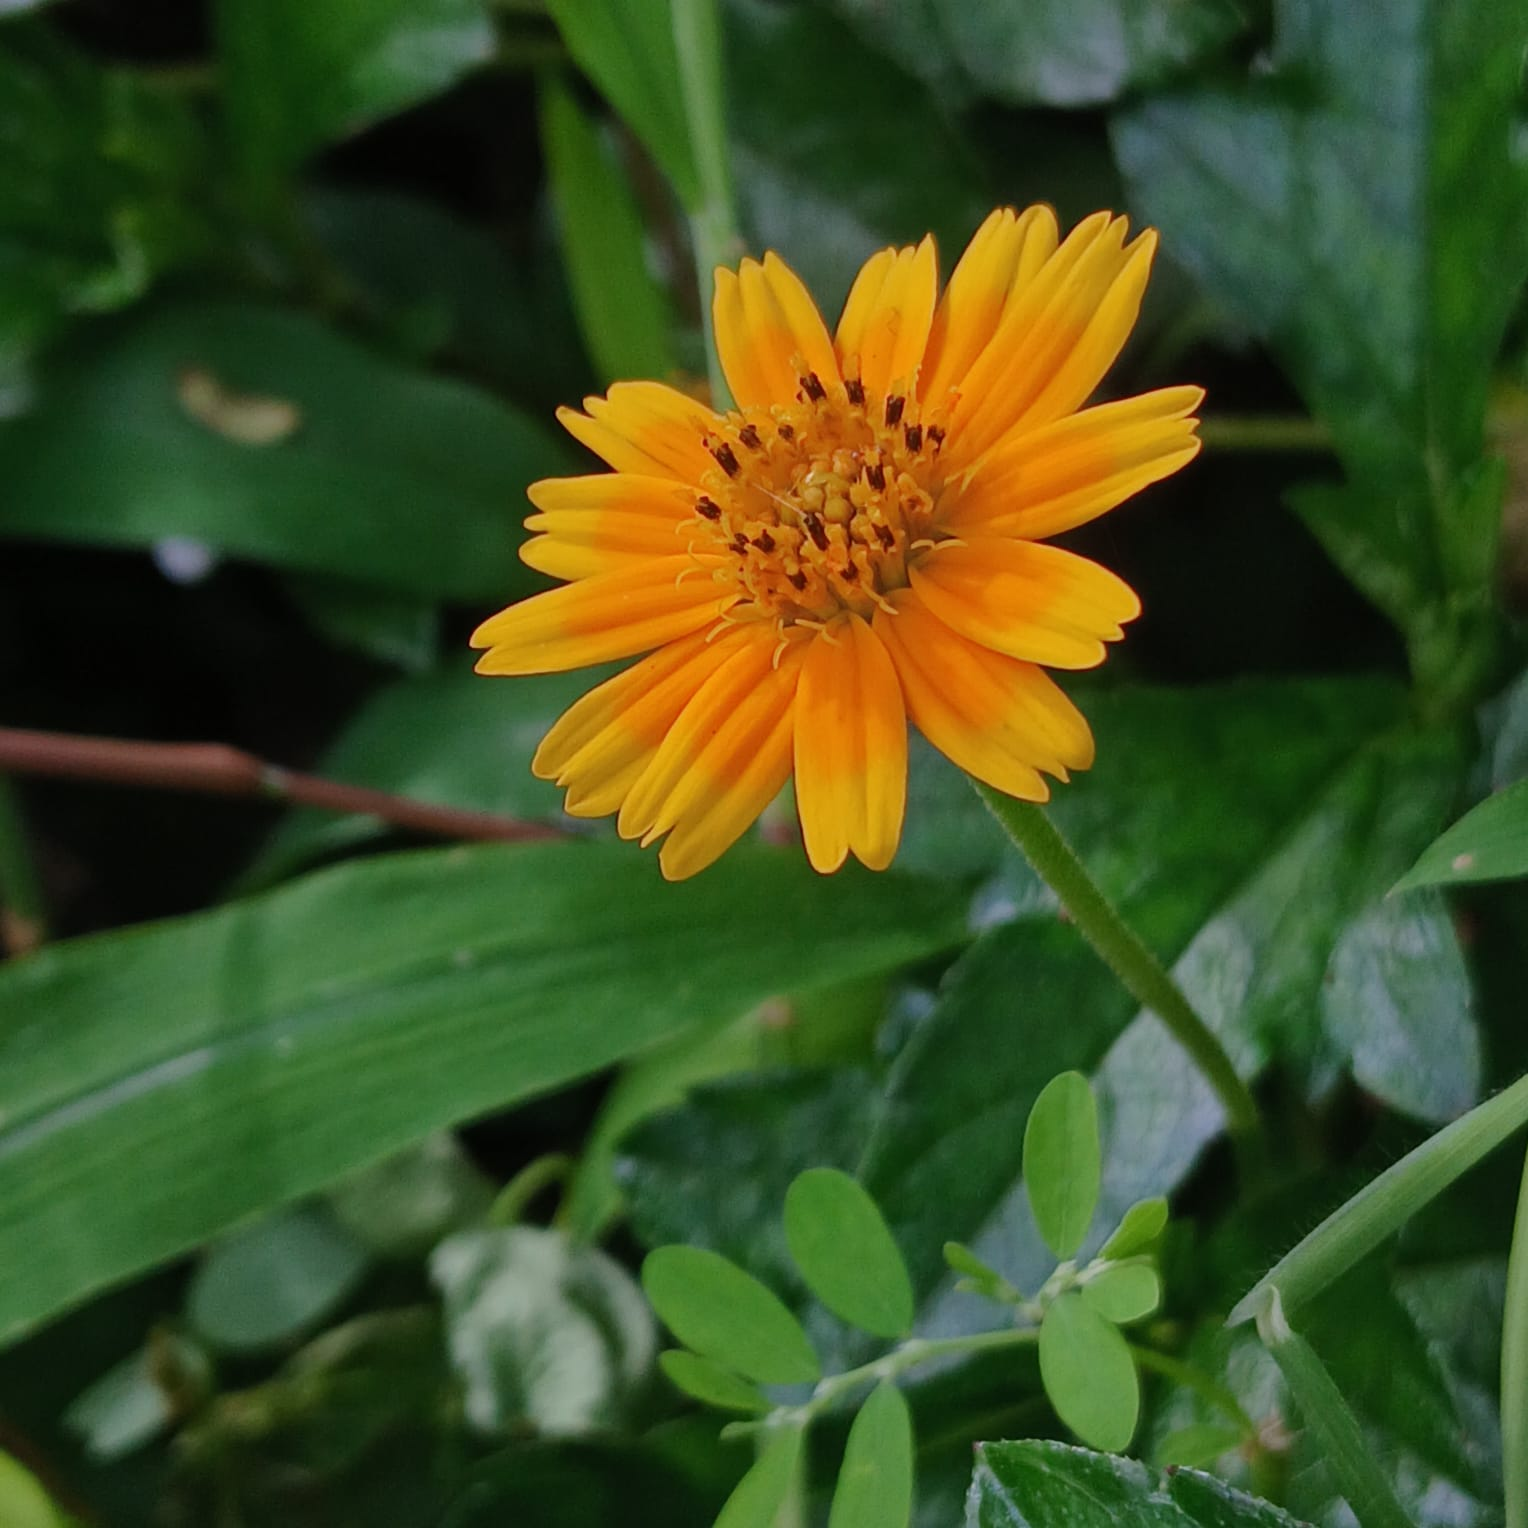
\includegraphics[width=0.6\textwidth]{Wedelia.jpg}
			\captionof{figure}{\ifnt{Wedelia sp.}}
		\end{center}
		
		\begin{center}
			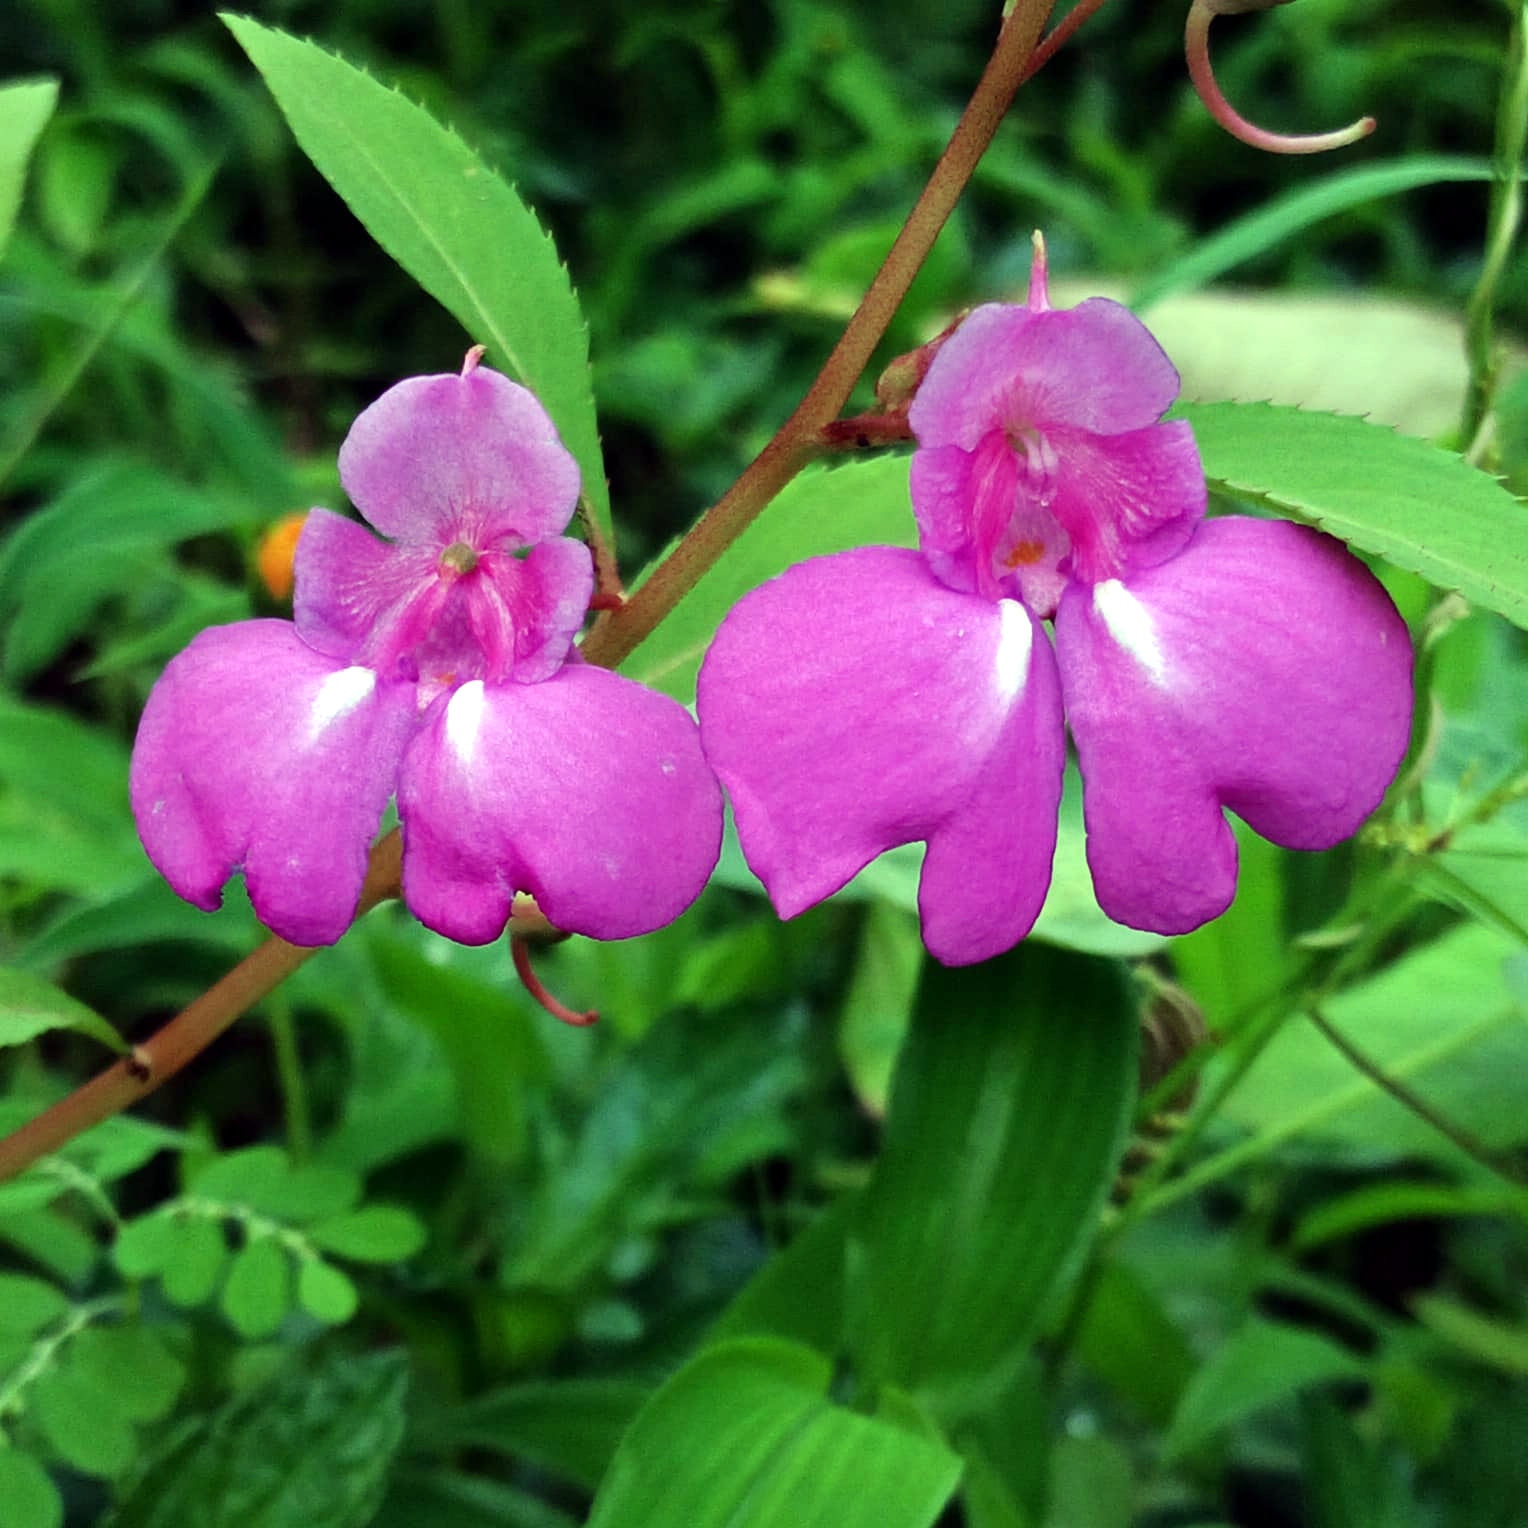
\includegraphics[width=0.6\textwidth]{Balsam.jpg}
			\captionof{figure}{\ifnt{Impatiens balsamina} aka. Balsam}
			
			\vspace*{1.2cm}
			
			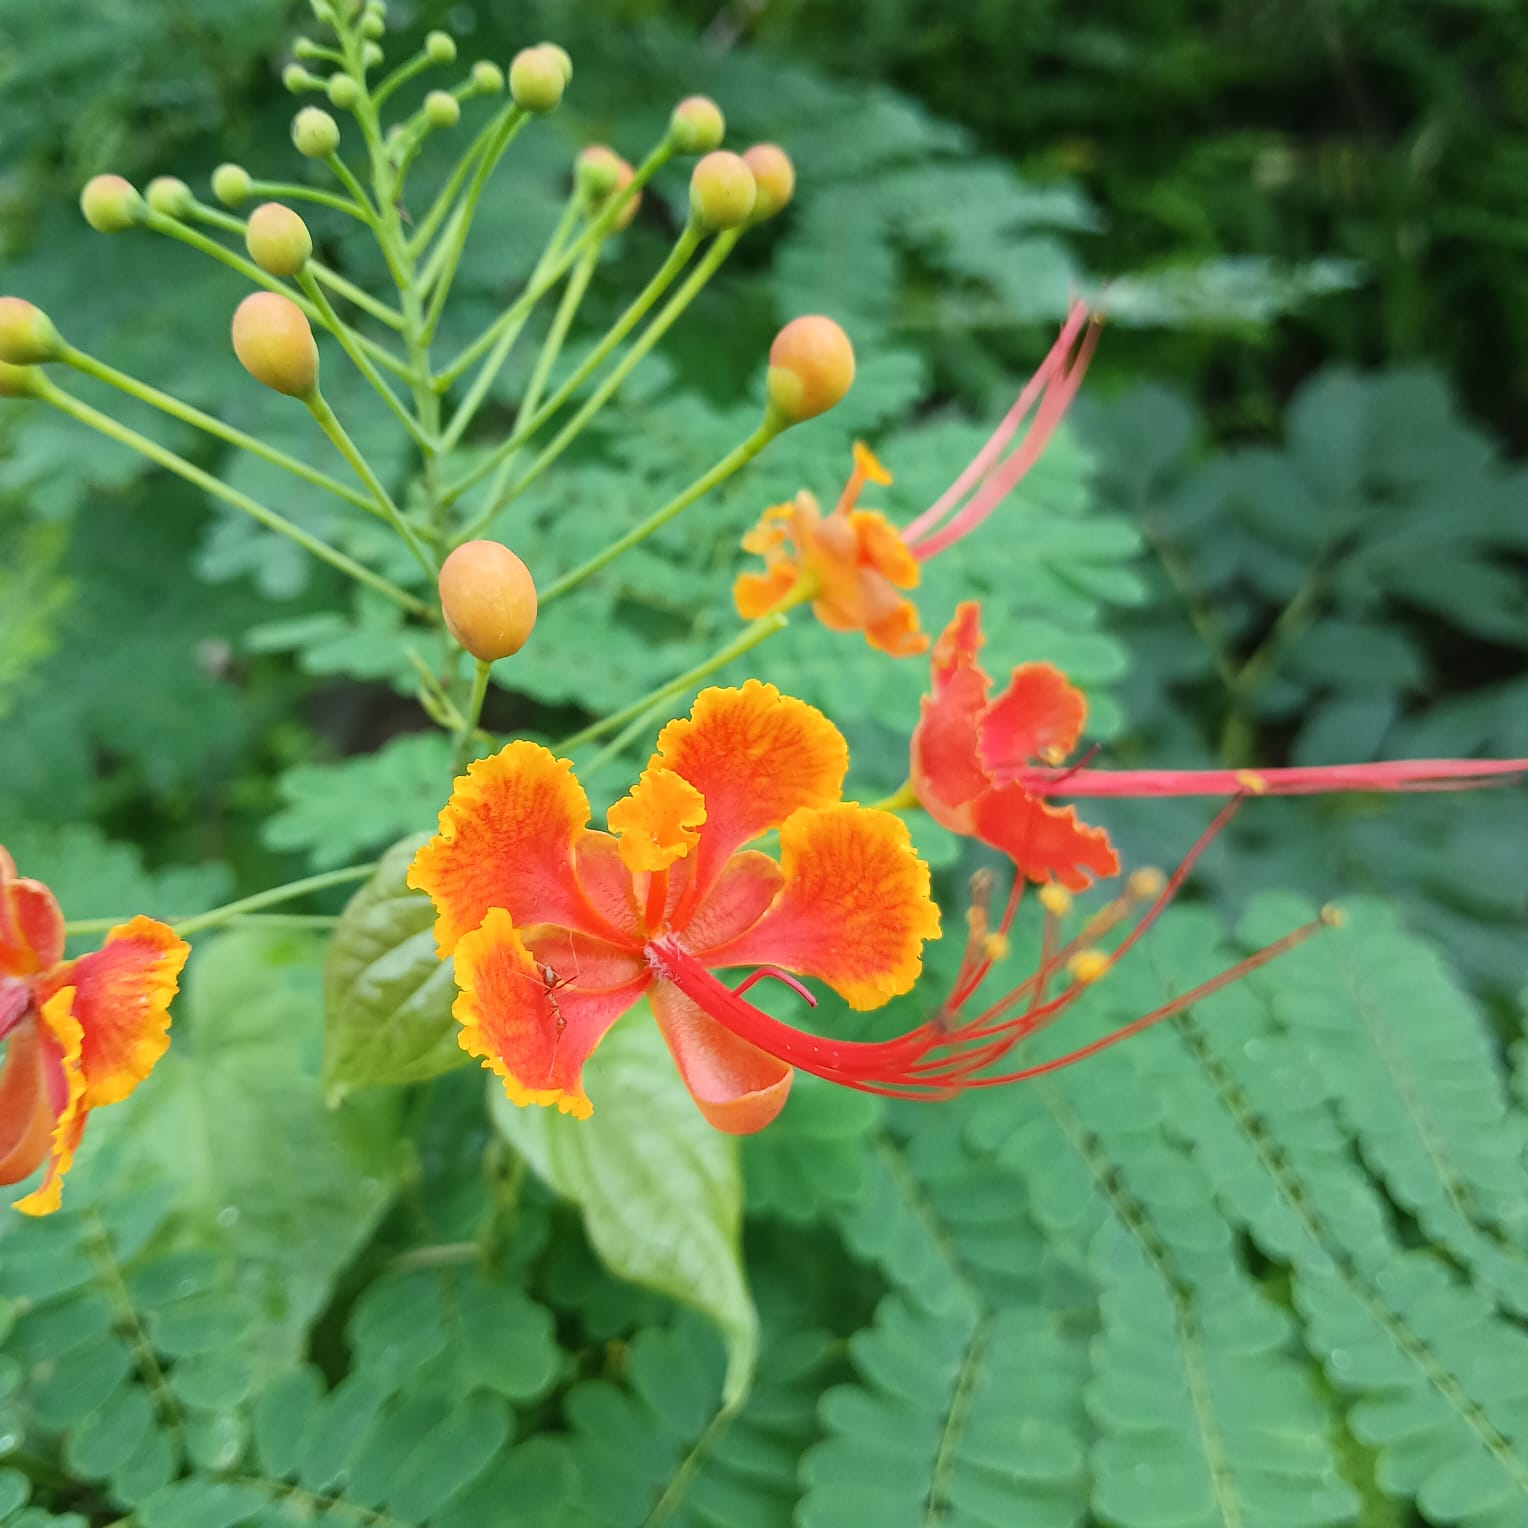
\includegraphics[width=0.6\textwidth]{Shankhasur.jpg}
			\captionof{figure}[\ifnt{Caesalpinia pulcherrima}]{\protect\ifnt{Caesalpinia pulcherrima} aka. Shankhasur flower,\\known as Krishnachura in Bengali.}
		\end{center}
		
		\clearpage
		
		\begin{center}
			\includegraphics[height=0.5\textwidth,angle=-90]{trail1.jpg}
			\vfill
			\includegraphics[width=0.8\textwidth]{trail2.jpg}
		\end{center}
		
		\clearpage
		
		\begin{center}
			\includegraphics[width=0.8\textwidth]{trail3.jpg}
			\vfill
			\includegraphics[height=0.55\textwidth,angle=-90]{trail4.jpg}
		\end{center}
		
		\clearpage
		
		\begin{center}
			
			\begin{minipage}[m]{0.45\textwidth}
				\includegraphics[width=\linewidth]{trail12.jpg}
			\end{minipage}\hfill%
			\begin{minipage}[m]{0.45\textwidth}
				\includegraphics[width=\linewidth]{trail13.jpg}
			\end{minipage}
			
			\vspace*{1cm}
			
			\includegraphics[width=0.9\textwidth]{trail14.jpg}
			
		\end{center}
		
		
		
		\begin{center}
			
			\includegraphics[width=0.8\textwidth]{trail15.jpg}
			
			\vspace*{0.5cm}
			
			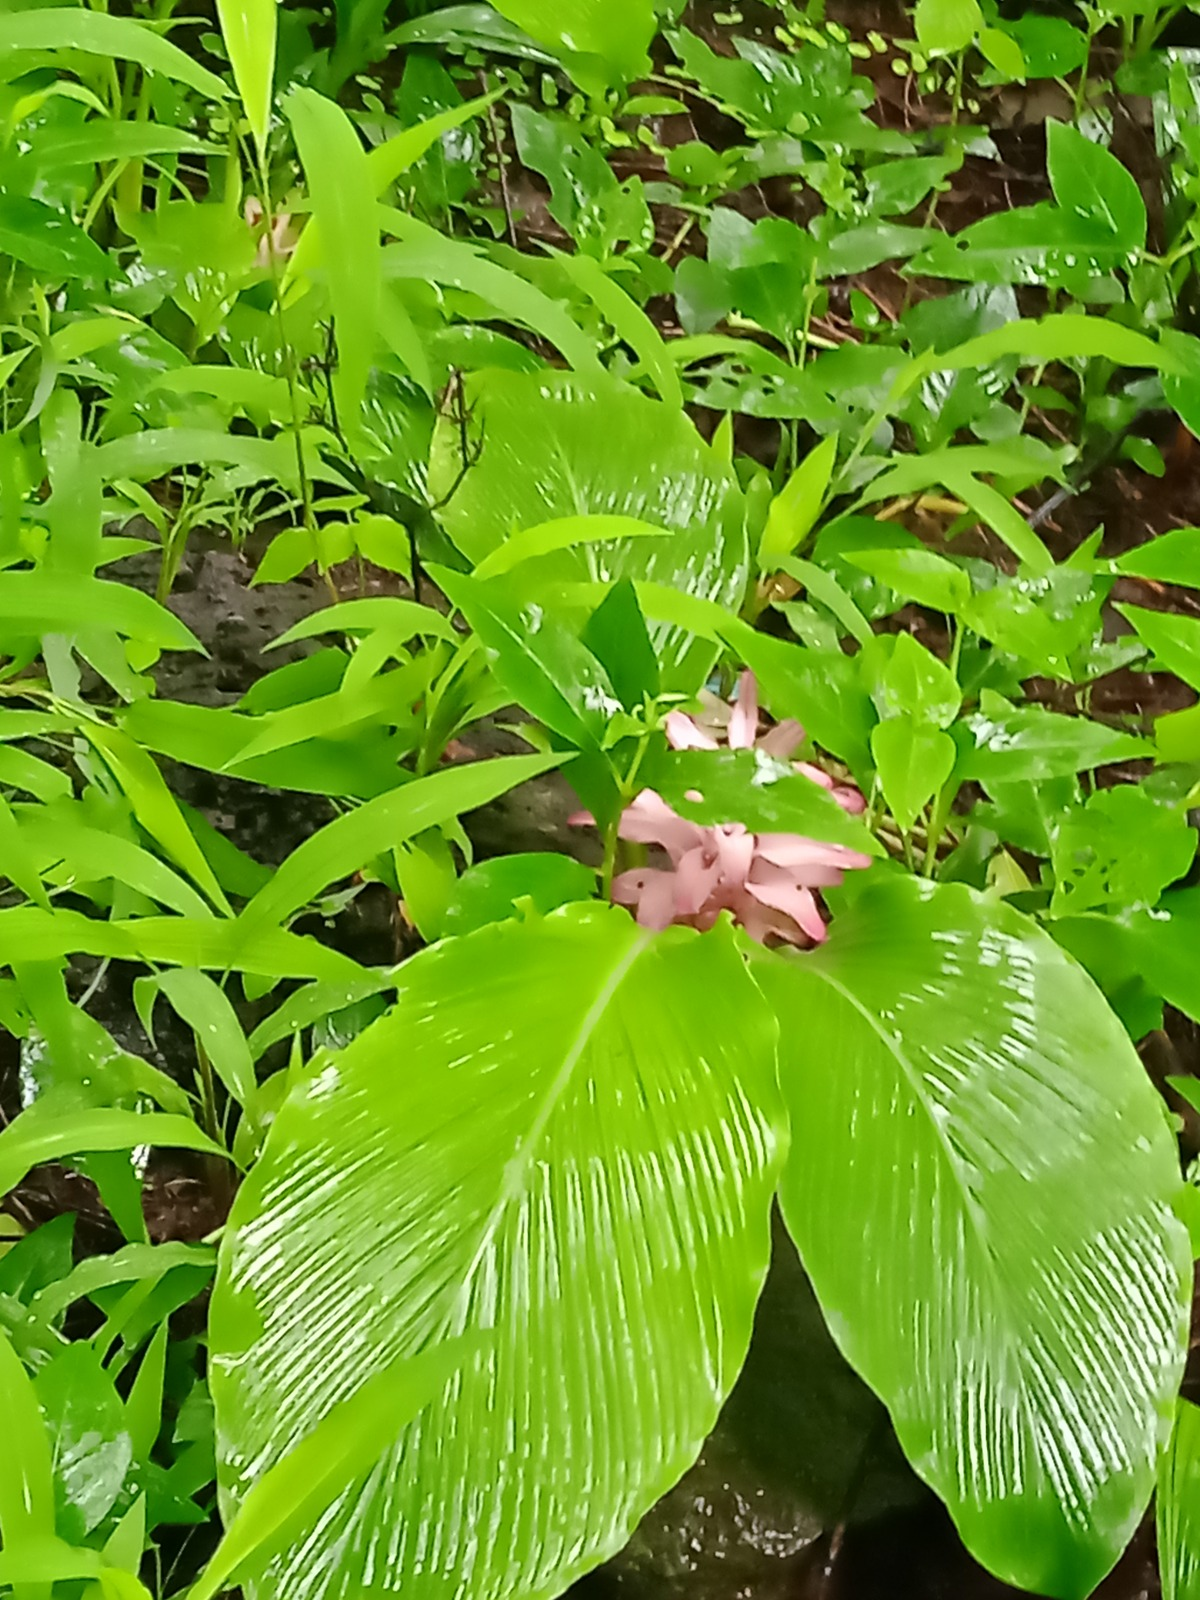
\includegraphics[width=0.4\textwidth]{ginger.jpg}
			\captionof{figure}[Wild ginger, \ifnt{Curcuma pseudomontana}]{Wild ginger, \ifnt{Curcuma pseudomontana}. The broad, oblong-elliptic leaf with a strong midrib and dense, parallel lateral veis running out to the margin at a narrow angle, and the sheathing leaf bases forming a pseudostem are all indicative of the ginger family, Zingiberaceae: Angiospermae\ \ \textrightarrow\ \ monocots\ \ \textrightarrow\ \ commelinids\ \ \textrightarrow\ \ Zingiberales\ \ \textrightarrow\ \ Zingiberaceae. The pink structures at the centre are not petals but bracts, and in \ifnt{Curcuma}, the upper sterile bracts form a brightly coloured coma while the true flowers sit lower down in the axils of the green bracts. The fact that it flowers with the first rains and was found in the western ghats is highly suggestive of the species \ifnt{Curcuma pseudomontana}.}
			
		\end{center}
		
		\clearpage
		
		\begin{center}
			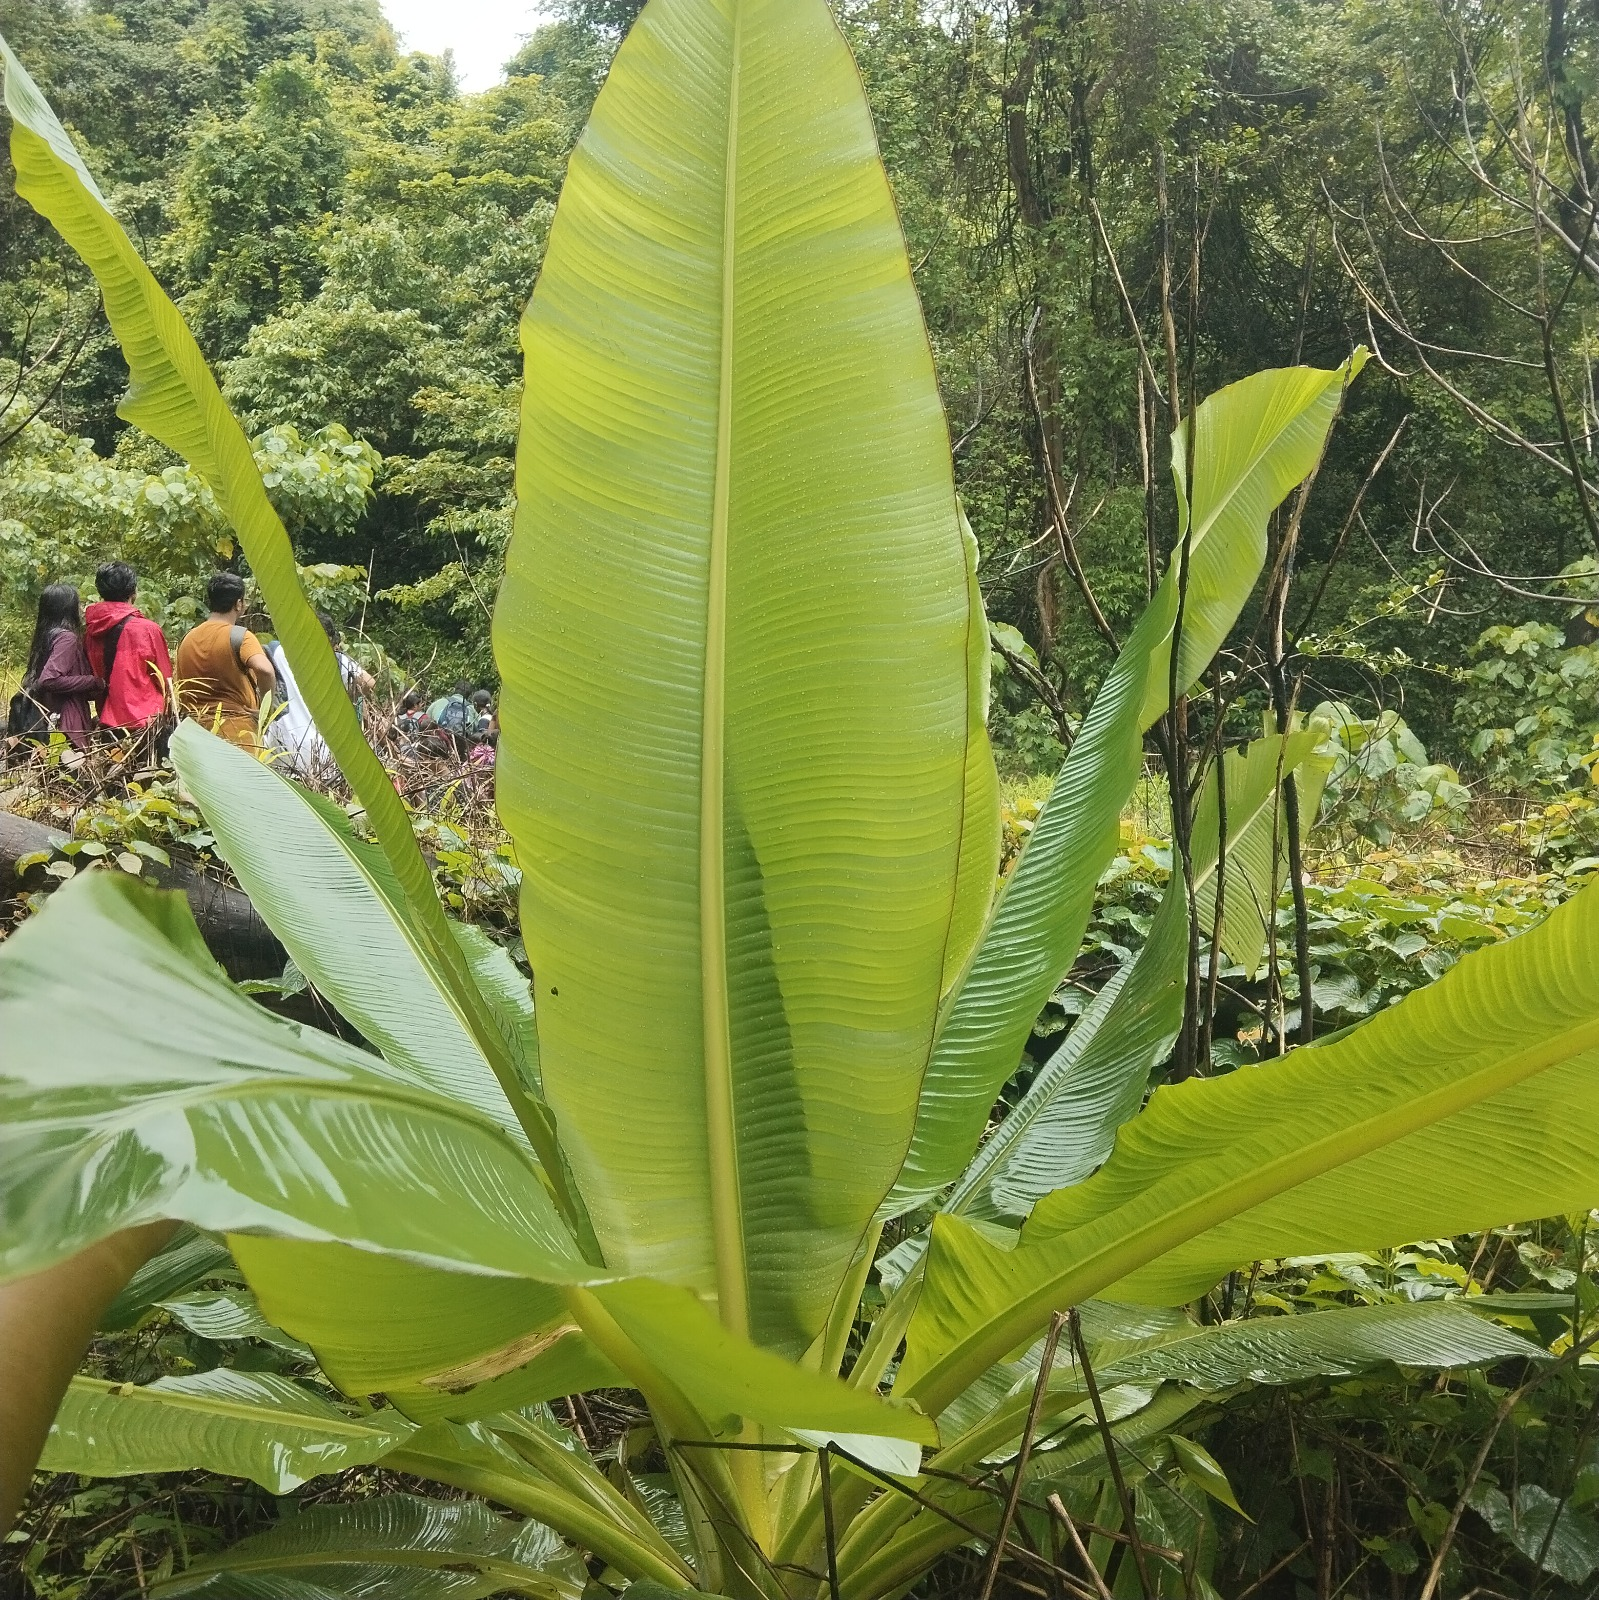
\includegraphics[width=0.5\textwidth]{banana.jpg}
			\captionof{figure}[\ifnt{Ensete}]{\ifnt{Ensete} Belongs to the same order as \ifnt{Curcuma}, but different family: Musaceae (Zingiberaceae: Angiospermae\ \ \textrightarrow\ \ monocots\ \ \textrightarrow\ \ commelinids\ \ \textrightarrow\ \ Musaceae). Identified from the leaf: a stout midrib with closely spaced parallel lateral veins running out at almost a right angle, unbranched, ending at the margin.}
			
			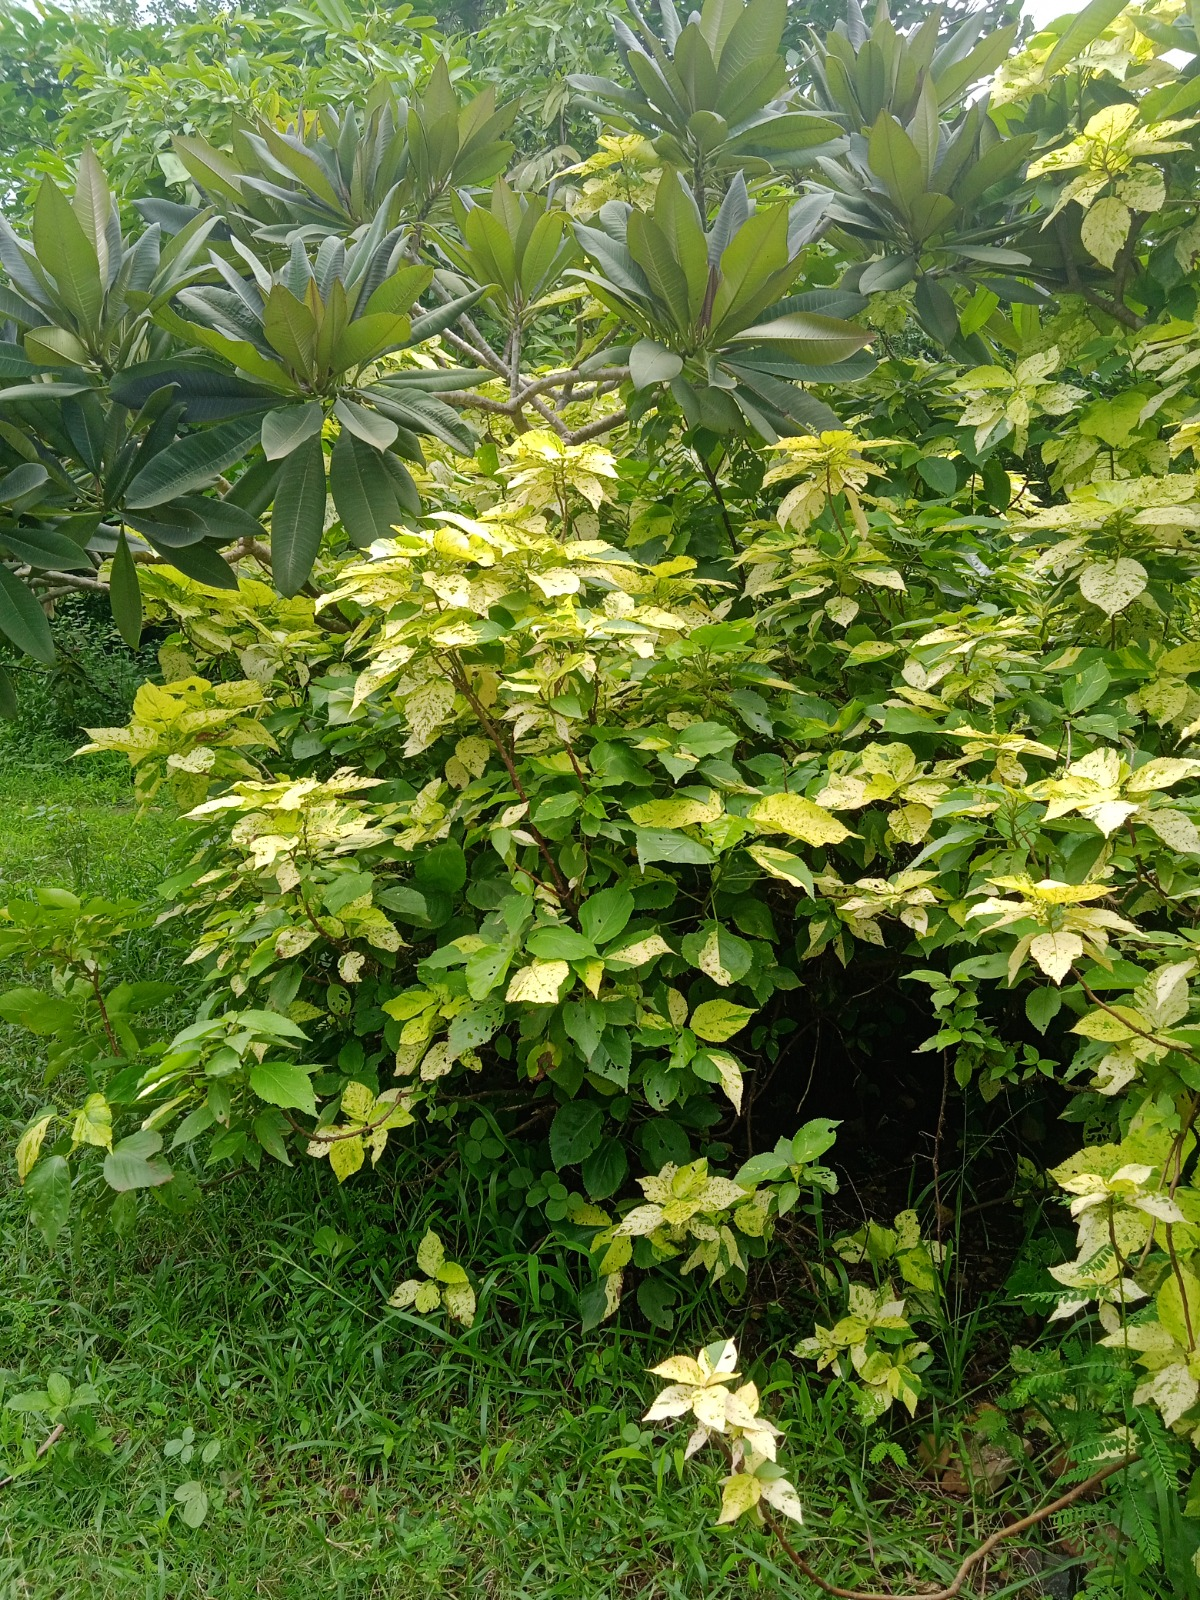
\includegraphics[width=0.5\textwidth]{Acalypha.jpg}
			\captionof{figure}[\ifnt{Acalypha wilkesiana}]{\ifnt{Acalypha wilkesiana}. Placement: Angiospermae\ \ \textrightarrow\ \ eudicots\ \ \textrightarrow\ \ rosids\ \ \textrightarrow\ \ fabids\ \ \textrightarrow\ \ Malpighiales\ \ \textrightarrow\ \ Euphorbiaceae, subfamily Acalyphoideae. Leaf colouration is a typical feature. Flowers appear as long inflorescences, resembling the tail of a cat. Hence called catkin inflorescence.}
			
		\end{center}
		
		\clearpage
		
		\topskip0pt
		\vspace*{\fill}
		\begin{center}
			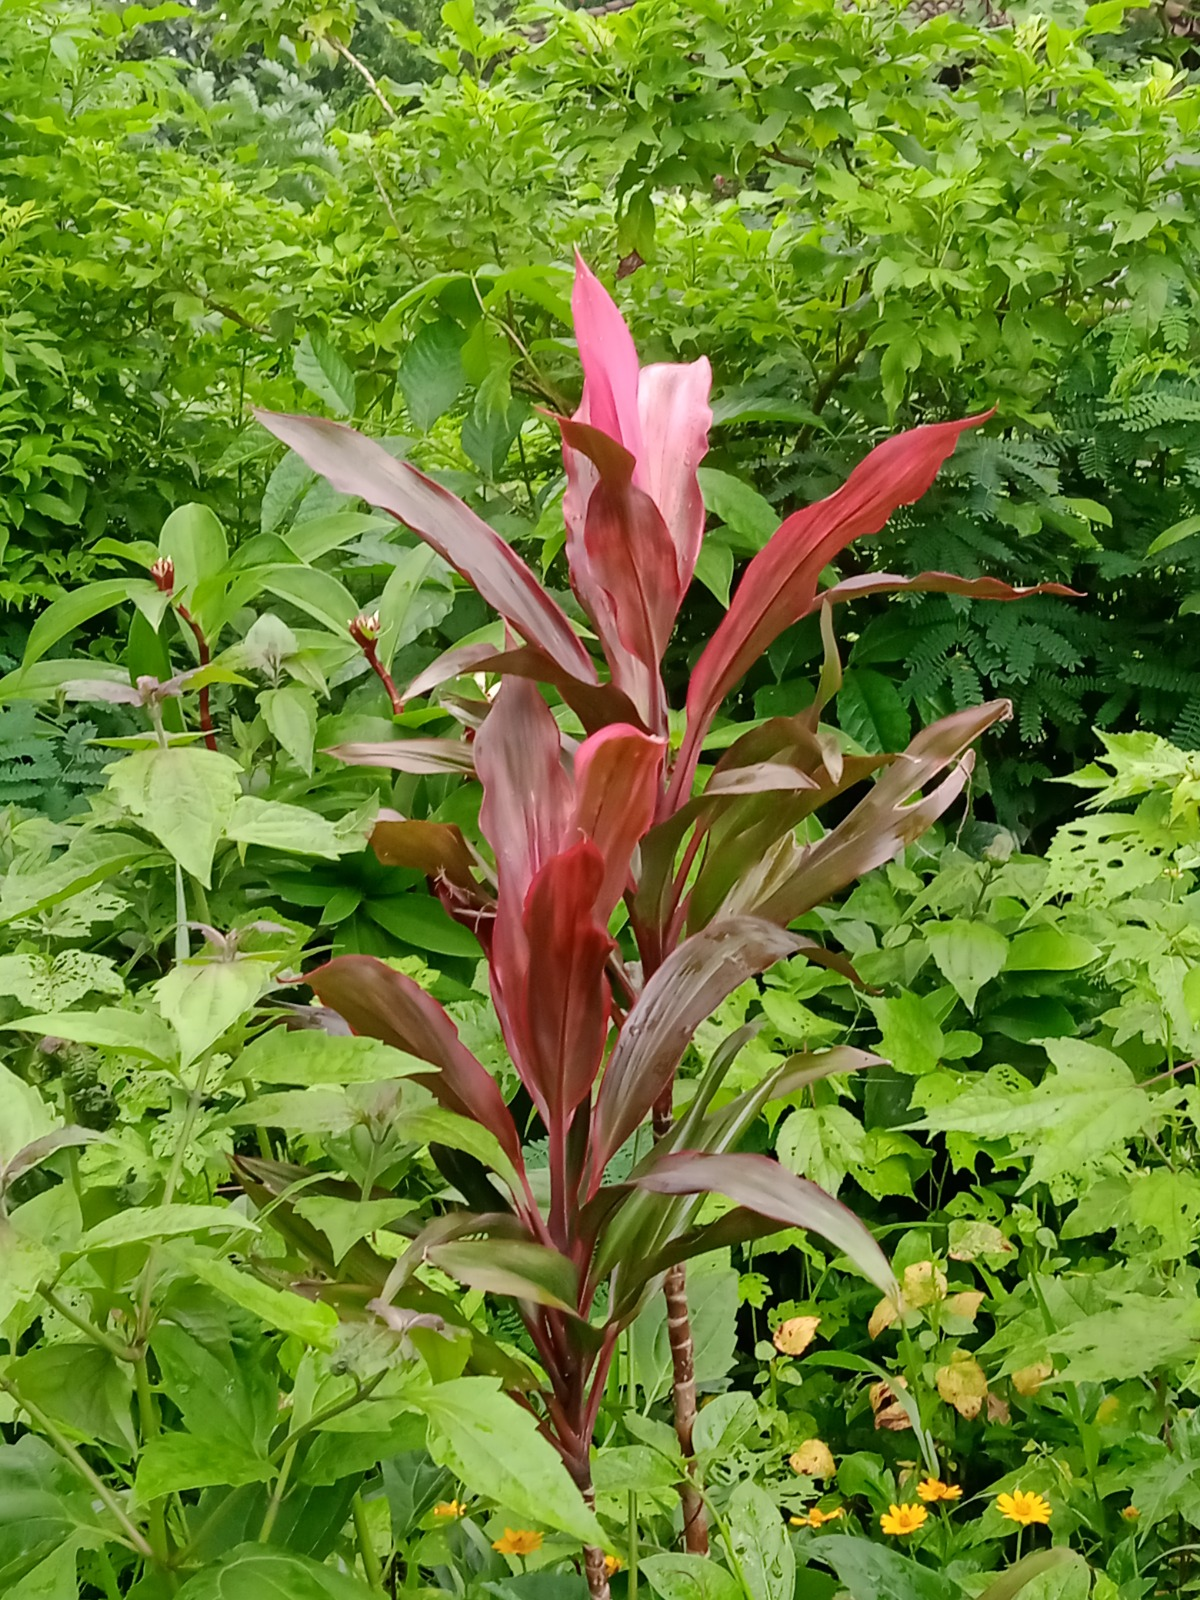
\includegraphics[width=0.6\textwidth]{Cordyline.jpg}
			\captionof{figure}[\ifnt{Cordyline fruticosa}]{\ifnt{Cordyline fruticosa}, the ti plant. Rarely seen in the wild. The red here is anthocyanin accumulating in the epidermis and mesophyll, overlying perfectly functional chlorophyll. The leaves photosynthesise normally. Placement: Angiospermae\ \ \textrightarrow\ \ monocots\ \ \textrightarrow\ \ Asparagales\ \ \textrightarrow\ \ Asparagaceae\ \ \textrightarrow\ \ subfamily Lomandroideae. \ifnt{Cordyline} has been shuffled around more than most plants. It has been placed in Liliaceae, Agavaceae, Dracaenaceae and Laxmanniaceae at various times. APG IV consolidated a large number of these small families into a broadly defined Asparagaceae with seven subfamilie. It is a monocot with a woody stem. Monocots have no vascular cambium and normally cannot thicken their stems. \ifnt{Cordyline}, \ifnt{Dracaena}, \ifnt{Yucca} and \ifnt{Aloe} get around this with a secondary thickening meristem, a distinct meristem outside the vascular bundles that produces whole new bundles embedded in parenchyma.}
		\end{center}
		\vspace*{\fill}
		
		\clearpage
		
		\topskip0pt
		\vspace*{\fill}
		\begin{center}
			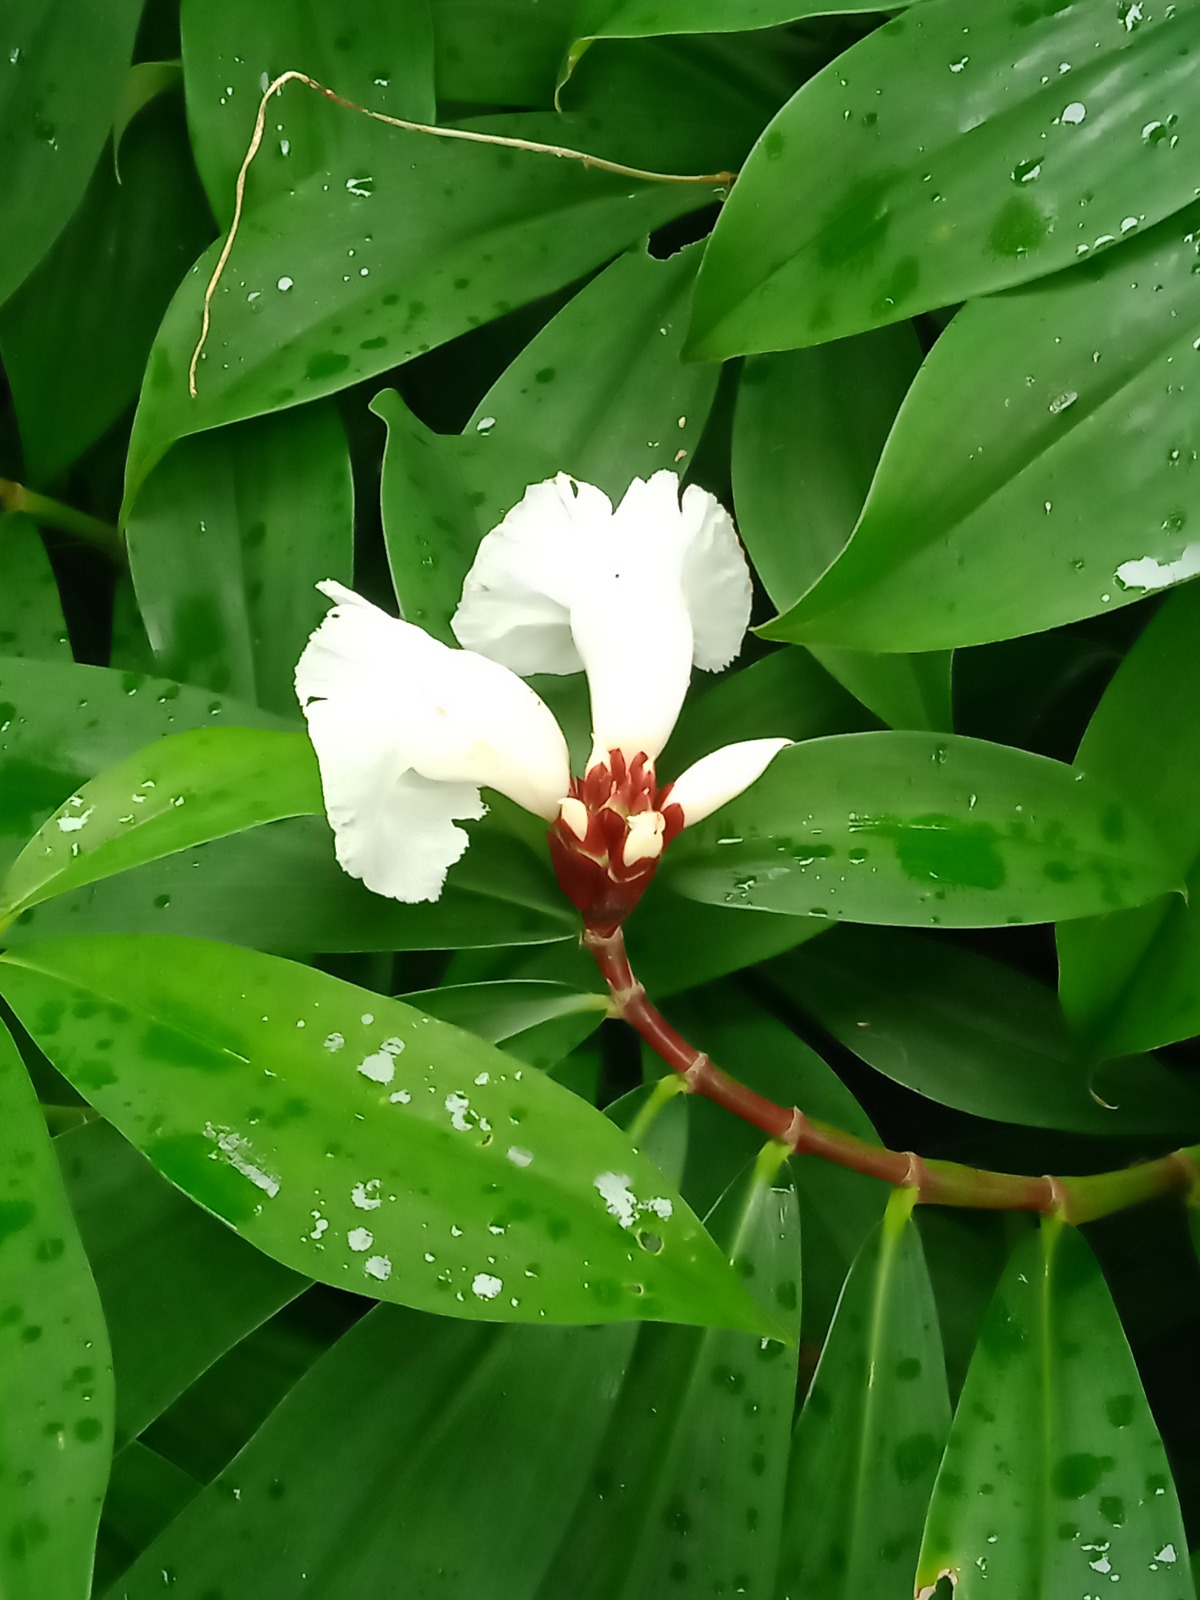
\includegraphics[width=0.6\textwidth]{Hellenia.jpg}
			\captionof{figure}[Crepe ginger or spiral ginger, \ifnt{Hellenia speciosa}]{\protect Crepe ginger or spiral ginger, \ifnt{Hellenia speciosa}. The species name has moved three times. It was originally \ifnt{Costus speciosus}, but was transferred to \ifnt{Cheilocostus speciosus} in 2006, and the currently accepted name in Plants of the World Online\footnotemark is \ifnt{Hellenia speciosa}, with \ifnt{Costus speciosus} and \ifnt{Cheilocostus speciosus} both listed as synonyms. Costaceae now recognises \ifnt{Hellenia} Retz. as the accepted genus with \ifnt{Cheilocostus} as its synonym.}
			
			\footnotetext{\url{https://powo.science.kew.org/taxon/urn:lsid:ipni.org:names:60469691-2}}
		\end{center}
		\vspace*{\fill}
		
		\clearpage
		
		\begin{center}
			\vfill
			\begin{minipage}[c]{0.45\textwidth}
				\includegraphics[height=\linewidth,angle=-90]{trail5.jpg}
			\end{minipage}\hfill%
			\begin{minipage}[c]{0.45\textwidth}
				\includegraphics[height=\linewidth,angle=-90]{trail6.jpg}
			\end{minipage}
			\vfill
			\begin{minipage}[c]{0.45\textwidth}
				\includegraphics[height=\linewidth,angle=-90]{trail7.jpg}
			\end{minipage}\hfill%
			\begin{minipage}[c]{0.45\textwidth}
				\includegraphics[height=\linewidth,angle=-90]{trail8.jpg}
			\end{minipage}
			\vfill
		\end{center}
		
		\clearpage
		
		\begin{center}
			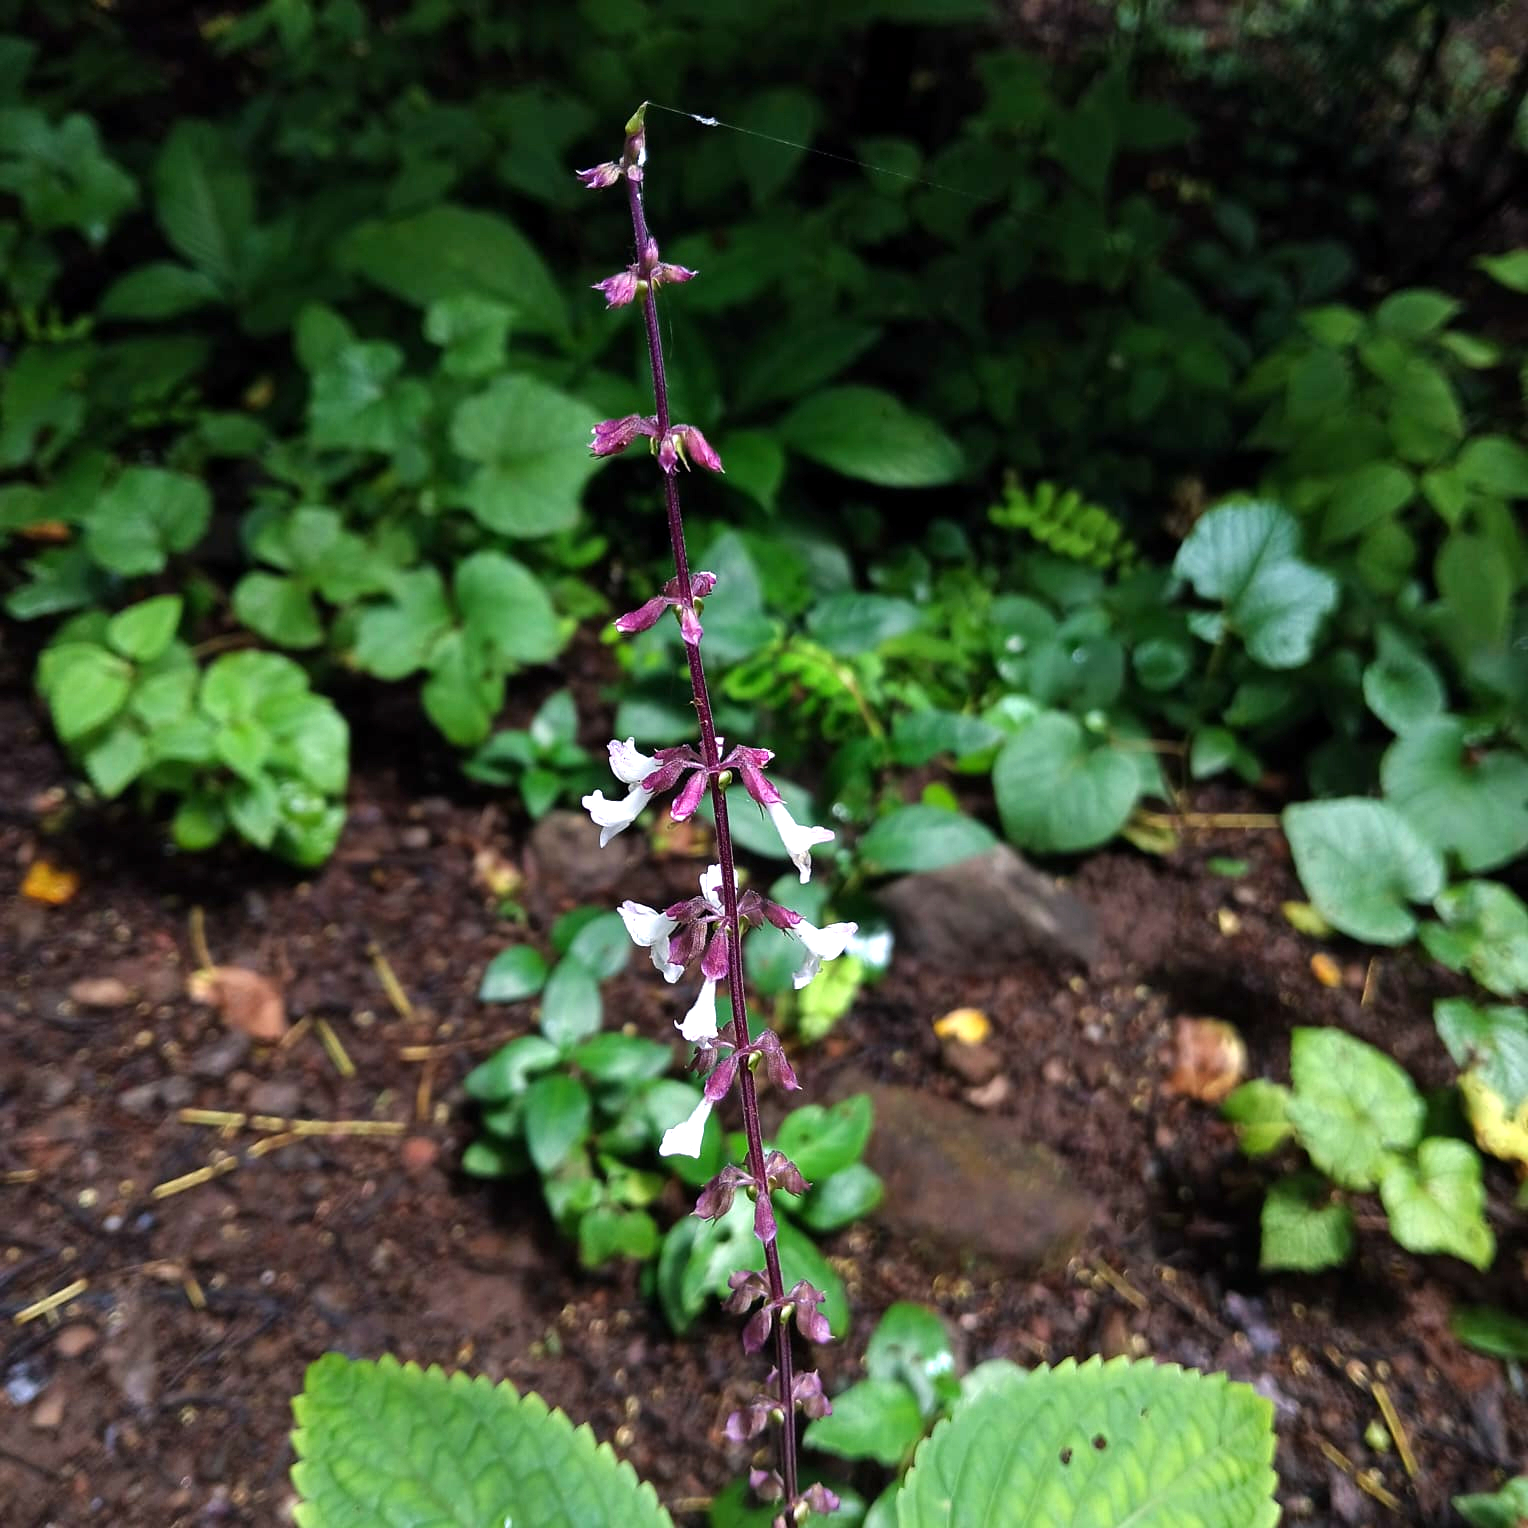
\includegraphics[width=0.7\textwidth]{Ocimum.jpg}
			\captionof{figure}[\ifnt{Ocimum tenuiflorum}]{\ifnt{Ocimum tenuiflorum}, a wild form of tulsi. Placement: Lamiales\ \ \textrightarrow\ \ Lamiaceae, subfamily Nepetoideae, tribe Ocimeae.}
			
			\vfill
			
			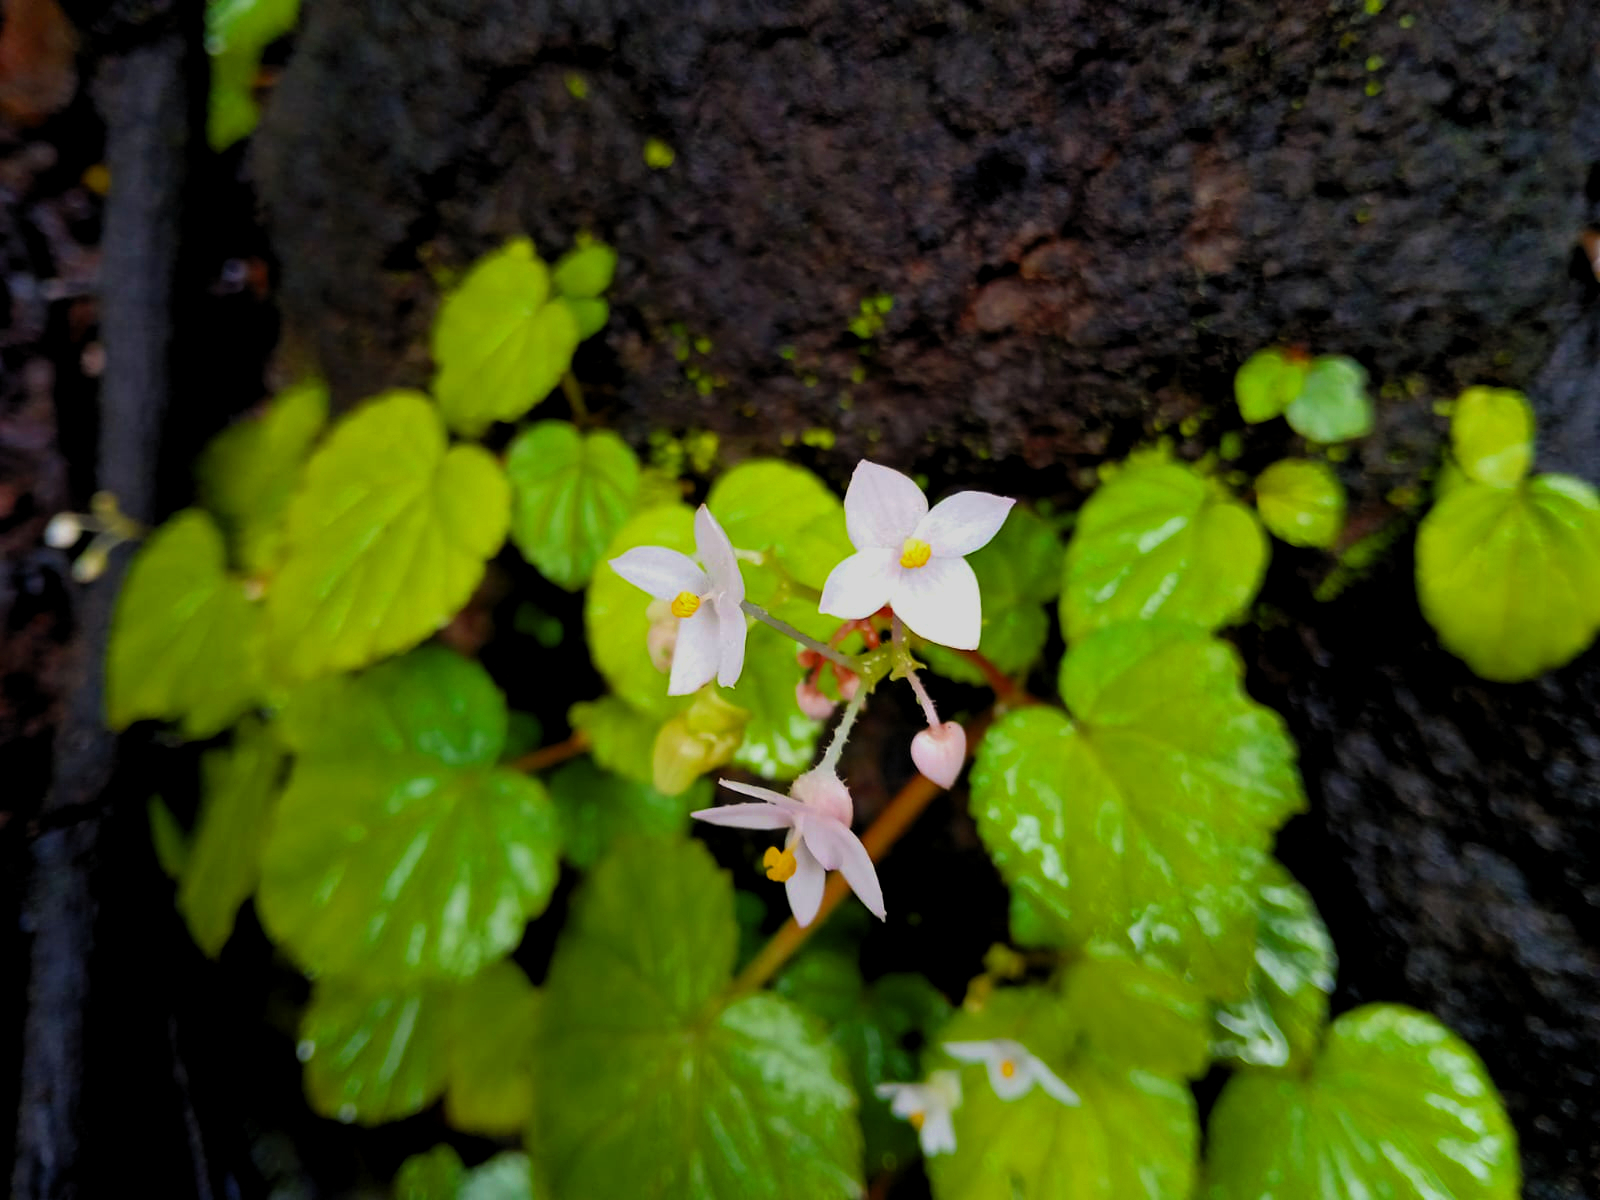
\includegraphics[width=0.7\textwidth]{Begonia.jpg}
			\captionof{figure}[\ifnt{Begonia}]{\ifnt{Begonia}. Placement: Angiospermae\ \ \textrightarrow\ \ eudicots\ \ \textrightarrow\ \ rosids\ \ \textrightarrow\ \ fabids\ \ \textrightarrow\ \ Cucurbitales\ \ \textrightarrow\ \ Begoniaceae\ \ \textrightarrow\ \ \ifnt{Begonia}}
		\end{center}
		
		\clearpage
		
		\begin{center}
			\includegraphics[width=0.5\textwidth]{trail09.jpg}
			\vfill
			\includegraphics[width=0.5\textwidth]{trail10.jpg}
		\end{center}
		
		\clearpage
		
		\begin{center}
			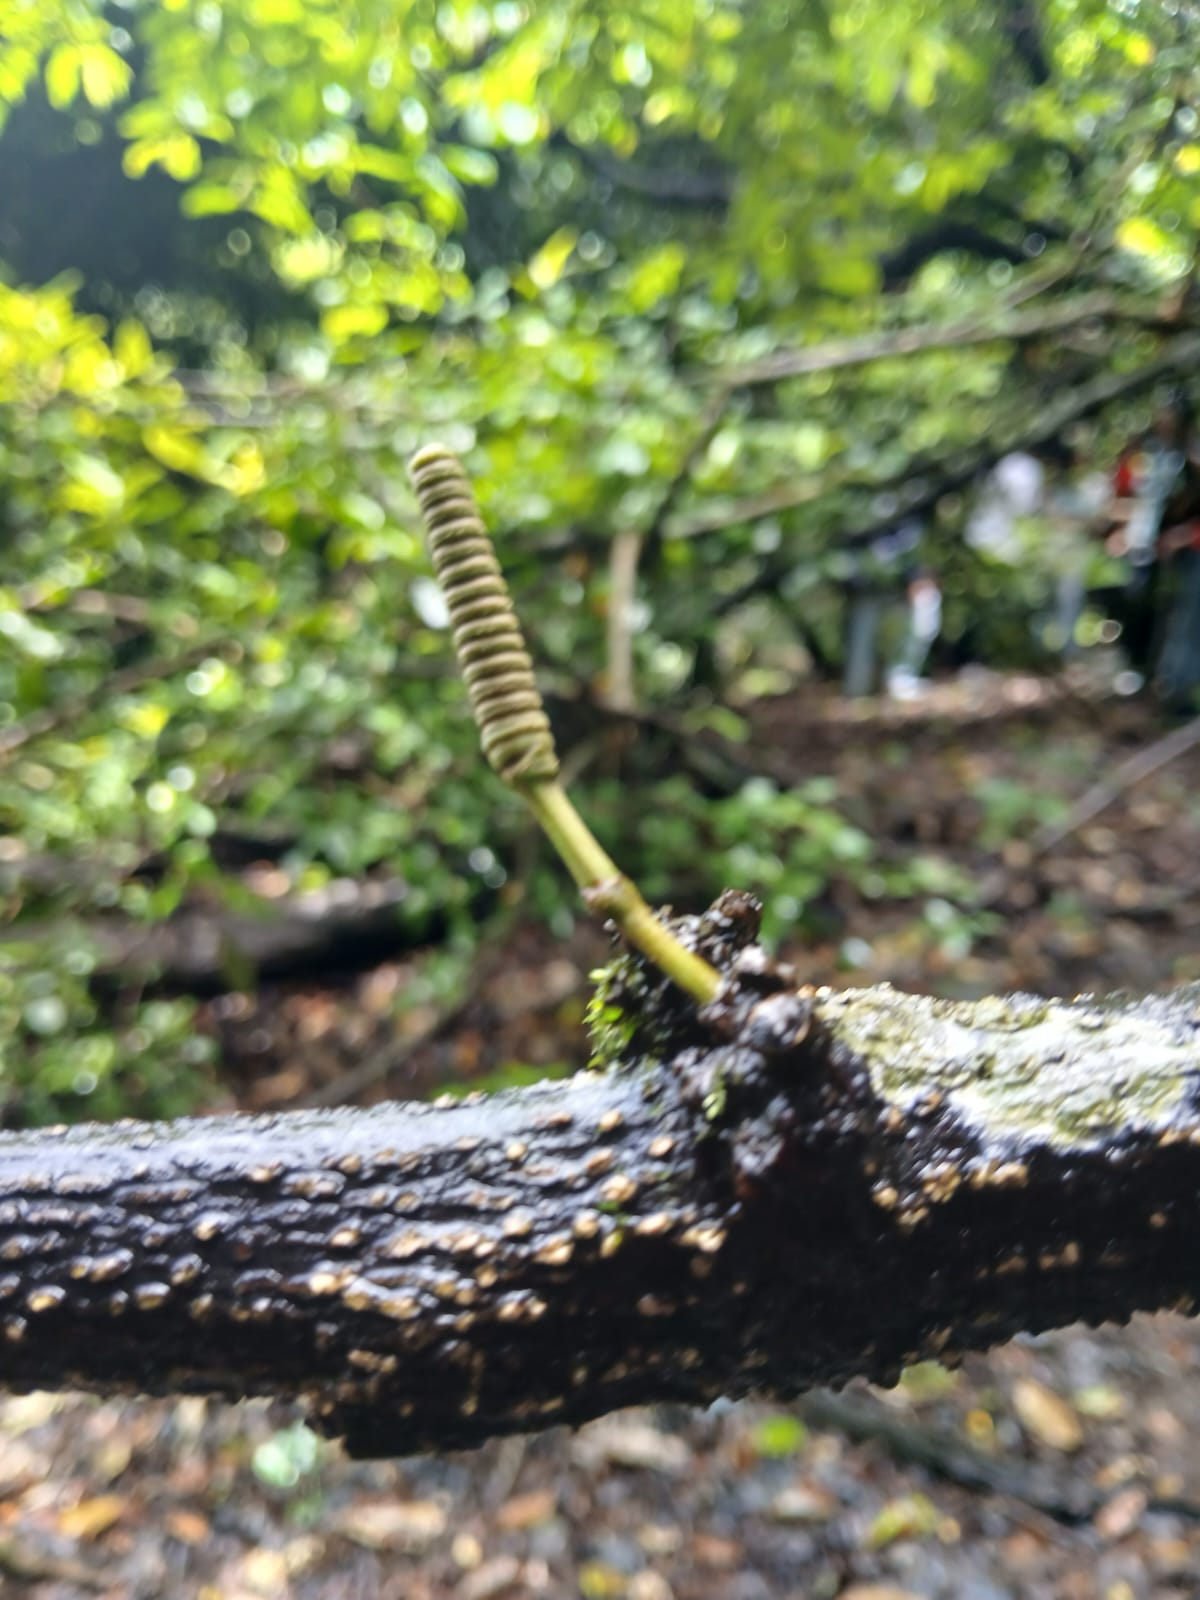
\includegraphics[width=0.5\textwidth]{Gnetum.jpg}
			\captionof{figure}[Cone of \ifnt{Gnetum}]{\label{fig:gnetum}A cone (primitive flower) of a gymnosperm named \ifnt{Gnetum}.}
		\end{center}
		
		Upon climbing the hill after the rain-fed spring, through the slippery rocks and mud in which our shoes were having a difficult time to find a grip on, we discovered the \ifnt{Gnetum} tree. It is an advanced gymnosperm and closer to the modern day plants, angiosperms. Hence unlike many other gymnosperms having needle shaped leaves, these have broad leaves similar to angiosperms. Also considered as an evolutionary connecting link between gymnosperms and angiosperms.\\
		
		\ifnt{Gnetum} confused botanists for nearly a century. It carries a set of angiosperm-like characters that no other gymnosperm has:
		
		\begin{itemize}
			
			\item Broad, flat leaves with reticulate venation, opposite and decussate, looking exactly like a dicot leaf;
			
			\item Vessel elements in the xylem, absent from all other gymnosperms except \ifnt{Ephedra} and \ifnt{Welwitschia};
			
			\item A double fertilisation of sorts, where the second male gamete fuses with another nucleus, though it does not produce endosperm;
			
			\item Strobili sometimes described as flower-like, with a perianth-like envelope around the ovule;
			
			\item Absence of archegonia in \ifnt{Gnetum}, unusual among gymnosperms.
			
		\end{itemize}
		
		That combination led to the anthophyte hypothesis, which placed Gnetales as sister to angiosperms. Molecular data demolished it, however. Gnetales now come out inside or beside the conifers, and all those angiosperm-like features are convergent. The reticulate venation and the vessels evolved independently. This is one of the cleanest textbook cases of morphological convergence misleading classification for decades.
		
		\clearpage
		
		\begin{center}
			\includegraphics[width=0.5\textwidth]{Ficus.jpg}
			\captionof{figure}[\ifnt{Ficus racemosa}]{\ifnt{Ficus racemosa}. Placement: Angiospermae\ \ \textrightarrow\ \ eudicots\ \ \textrightarrow\ \ rosids\ \ \textrightarrow\ \ fabids\ \ \textrightarrow\ \ Rosales\ \ \textrightarrow\ \ Moraceae\ \ \textrightarrow\ \ \ifnt{Ficus}. \ifnt{Ficus racemosa} is strongly riparian, favouring stream banks and moist ravines, and it is often treated as an indicator of shallow groundwater. Fig trees fruit asynchronously. That produces a continuous year-round food supply at the landscape scale, which sustains frugivores through the lean season when almost nothing else is fruiting. Ecologists therefore classify figs as keystone resources in tropical forests. \ifnt{Ficus racemosa} alone feeds hornbills, barbets, bulbuls, civets, macaques, langurs and fruit bats, and the fallen figs feed fish and ungulates.}
			\vfill
			
			\includegraphics[width=0.7\textwidth]{trail17.jpg}
		\end{center}
		
		\clearpage
		
		\begin{center}
			\includegraphics[width=0.9\textwidth]{trail18.jpg}
			\vfill
			\includegraphics[width=0.9\textwidth]{trail19.jpg}
		\end{center}
		
		\clearpage
		
		\topskip0pt
		\vspace*{\fill}
		\begin{center}
			\includegraphics[width=\textwidth]{trail20.jpg}
		\end{center}
		\vspace*{\fill}
		
		\clearpage
		
		\begin{center}
			\includegraphics[width=0.9\textwidth]{trail21.jpg}
		\end{center}
		
		\vspace{1cm}
		
		Thereafter, we returned to Yusuf Meherally Center for lunch.
		
		\clearpage
		
	\section{Yusuf Meherally Center}
		
		The Yusuf Meherally Center sits at Tara village, near Karnala, in Taluka Panvel, District Raigad, Maharashtra, about 18 km from Panvel in Navi Mumbai, on the Mumbai to Goa road. It is a registered voluntary organization under the Societies Registration Act, 1860 and the Bombay Public Trust Act, 1950.\\
		
		The Centre is named in memory of Yusuf Meherally (1903 -- 1950), a socialist freedom fighter who was elected Mayor of Bombay in 1942 while imprisoned in Yerawada Central Prison, and who founded the National Militia, the Bombay Youth League and the Congress Socialist Party. He is best remembered for coining two of the independence movement's most famous slogans. In 1928 he came up with "Simon Go Back" in protest against the all-British Simon Commission, and on 14 July 1942 he coined the slogan "Quit India," which was approved by Gandhi at Wardha. He was imprisoned eight times during the freedom struggle. He died young, at 47, in 1950. The Centre was set up by his associates so his name and ideals would not be forgotten. One of its co-founders, G. G. Parikh, put it plainly: ``We wanted to ensure that Yusuf Meherally's name is not forgotten. Many people volunteered to join and start the centre. Back then the purpose of the centre was to work towards 'national integration' and to bring people together across divisions."\\
		
		Over time its mission sharpened from "national integration" into rural development, driven by a specific diagnosis of India's problems. As Parikh described it, the centre came to focus on problems emerging from rapid urbanisation in Mumbai, and concluded that the solutions to the problems of urbanization lie not in the cities but in the hinterland: rural areas need to develop and have basic amenities so that people stay there, and no one should have to leave their village because they have no other option. The founding philosophy holds that development of India means rural development, that the right to work is a fundamental right, and that free and compulsory education plus community health and medical aid should be available to all equally.\\
		
		The Centre runs a cluster of village industries at Tara, most started decades ago, that turn local raw materials into everyday products while creating non-farm employment. The dated timeline from YMC's own records shows how these were built up: the Ghani Oil Industry began in 1978, the Soap Unit in 1986, the Bakery unit in 1987, and Vermiculture in 1994. The main ones include:%
%		
		\begin{itemize}
			
			\item Tel Ghani (traditional oil pressing);
			
			\item Handmade soap unit;
			
			\item Pottery;
			
			\item Vermiculture and vermi-composting; and
			
			\item Carpentry, from recycled wood (mostly teak).
			
		\end{itemize}
		
		Alongside the manufacturing units are agriculture and organic-farming operations, including paddy, vegetable cultivation and a nursery of medicinal plants, and biogas energy demonstrations.\\
		
		The products are sold both on site and through wider markets. Pottery, handmade soaps and oils are all available at the Centre, and it has also learned to market not only its own goods but the products of other village industries.\\
		
		What makes these more than a craft shop is the deliberate development philosophy behind them. The Centre rejects the Western industrial model outright. As Parikh argued, the Western model of development is an energy-guzzling machine that isn't sustainable. In its place YMC defines rural development as a specific formula: micro-watershed development plus organic farming plus non-conventional energy plus village industries and marketing their products, a definition drawn from nearly two and a half decades of experience.\\
		
		The reasoning for decentralized small industry is spelled out in the Centre's own model. Producing goods in a decentralized manner has become possible with the advance of technology, and with the rising costs of pollution and destruction of ecology, small-scale production has become not only viable but a necessity. The Centre also argues that employment generation is better than doles, and that the country can be developed by developing the countryside, because a lot of wealth and a large number of jobs will be created, raising rural incomes and stimulating the wider economy.\\
		
		The industries are one arm of a much broader effort to make village life viable so people don't have to migrate to city slums. The full range of YMC's activities includes rural development, health care, education, empowering women and Adivasis, youth mobilization, employment generation, organic farming and vermiculture, and relief and rehabilitation. \\
		
		Concretely, the Centre helps the surrounding population through:
		
		\begin{itemize}
			
			\item \bfnt{Employment generation:} The village industries and organic farms give landless labourers, small farmers and tribal (Adivasi) families paid, local, non-farm work, so that no one has to leave their village because they have no other option.
			
			\item \bfnt{Healthcare:} Health services are among its core activities. YMC operates regular dispensaries, mobile clinics and eye camps, and has built a 30-bed cottage hospital, extending medical aid to communities that would otherwise have little access.
			
			\item \bfnt{Education and vocational training:} It started the Yusuf Meherally High School at Tara in 1990, and opened a Non-Formal Vocational Centre for Adivasis in 1995 teaching skills like auto-repairing, electric wiring and maintenance. It also runs a multi-skill residential training program, the DBRT, covering agriculture, engineering (fabrication, construction, carpentry), energy and environment (electrical, motor rewinding, surveying, solar, biogas), home and health (sewing, food processing), and animal husbandry (poultry, goat farming, dairy). These pass on the very skills the industries use, so training and livelihood reinforce each other.
			
			\item \bfnt{Watershed and ecological restoration:} Its technical cell promotes micro-watershed development across the Konkan districts. YMC has run micro-watershed programmes in Thane, Raigad, Sindhudurg and Ratnagiri, with the stated benefits that soil erosion will stop and productivity will go up, scarcity of drinking water, fodder, fuel and timber will reduce, and need-based emigration to urban areas will reduce.
			
			\item \ifnt{Women's empowerment and disaster relief:} Empowerment of women and Adivasis runs through the village industries and agriculture training, and the Centre has an established record in relief and rehabilitation after disasters.
			
		\end{itemize}
		
		In short, the Yusuf Meherally Centre was built to honour a freedom fighter by continuing his belief that India's real development lies in its villages. Its sustainable small industries are the practical expression of that belief: low-energy, local-material, employment-generating enterprises that, together with the Centre's health, education, watershed and training work, aim to make rural life prosperous enough that people can stay and thrive where they are, rather than migrating to overcrowded cities.
		
		\clearpage
		
		\begin{center}
			\vfill
			\begin{minipage}[c]{0.45\textwidth}
				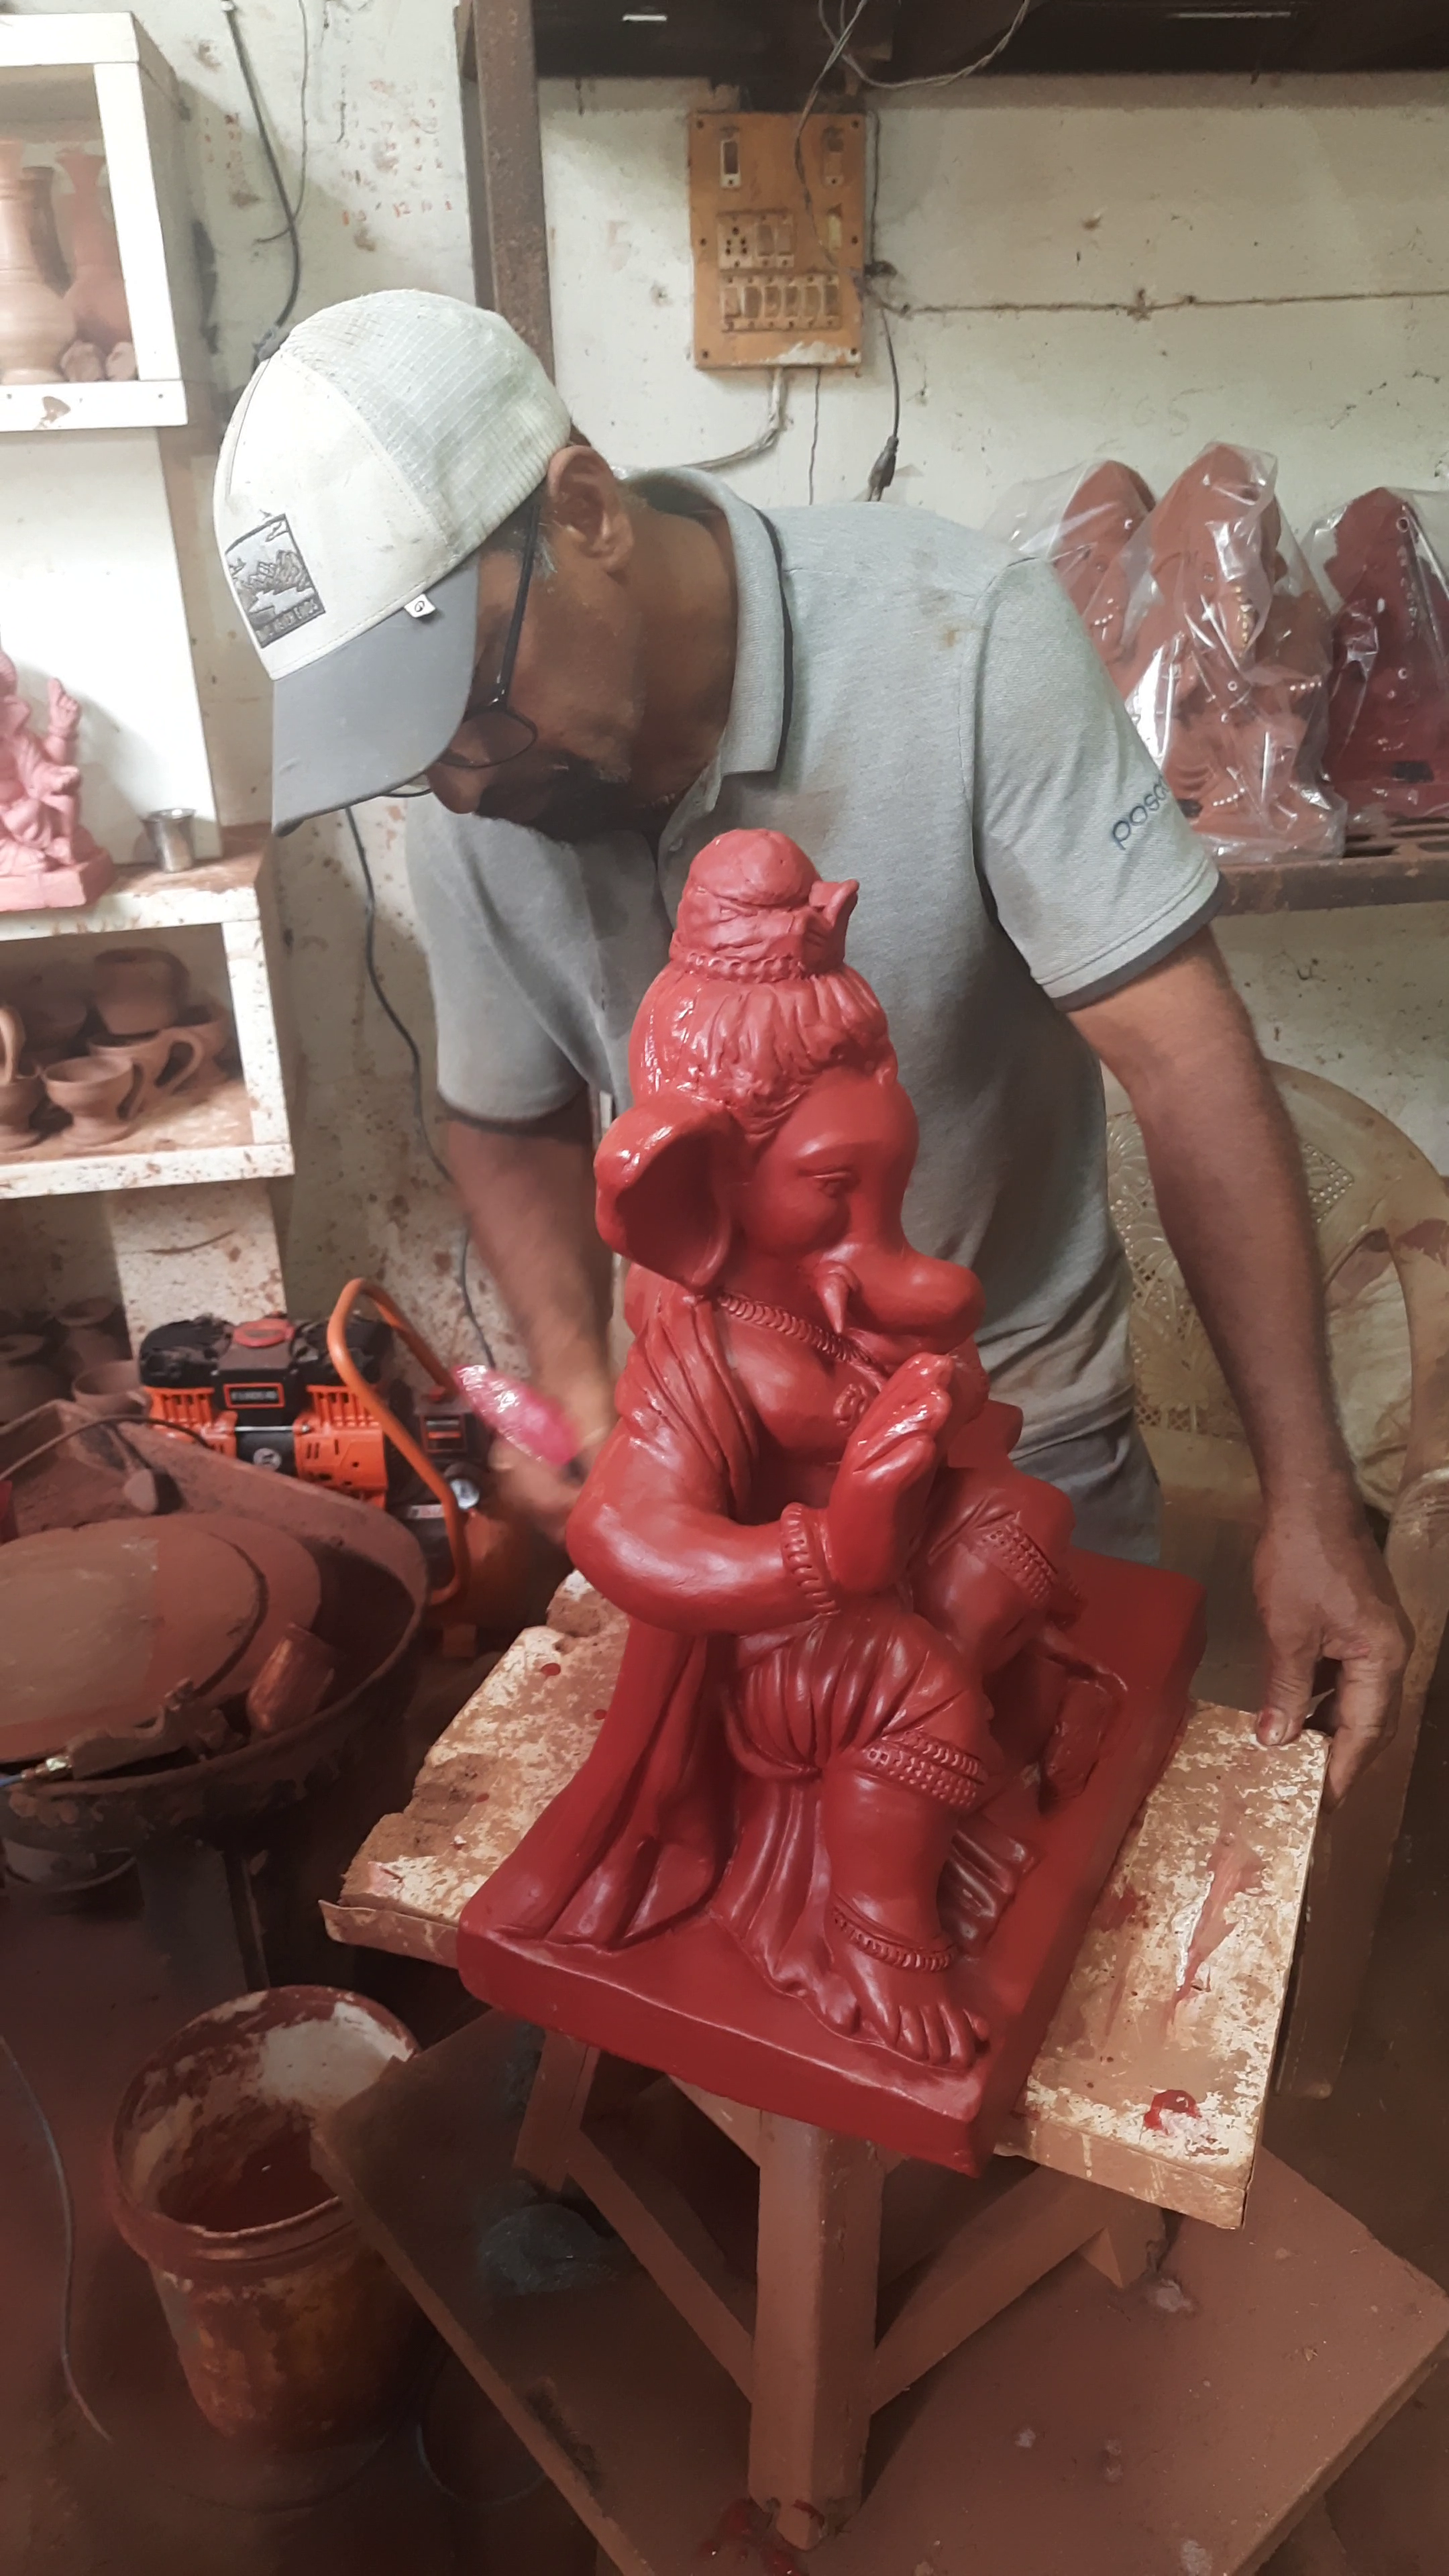
\includegraphics[width=0.8\linewidth]{pottery1.png}
			\end{minipage}\hfill%
			\begin{minipage}[c]{0.45\textwidth}
				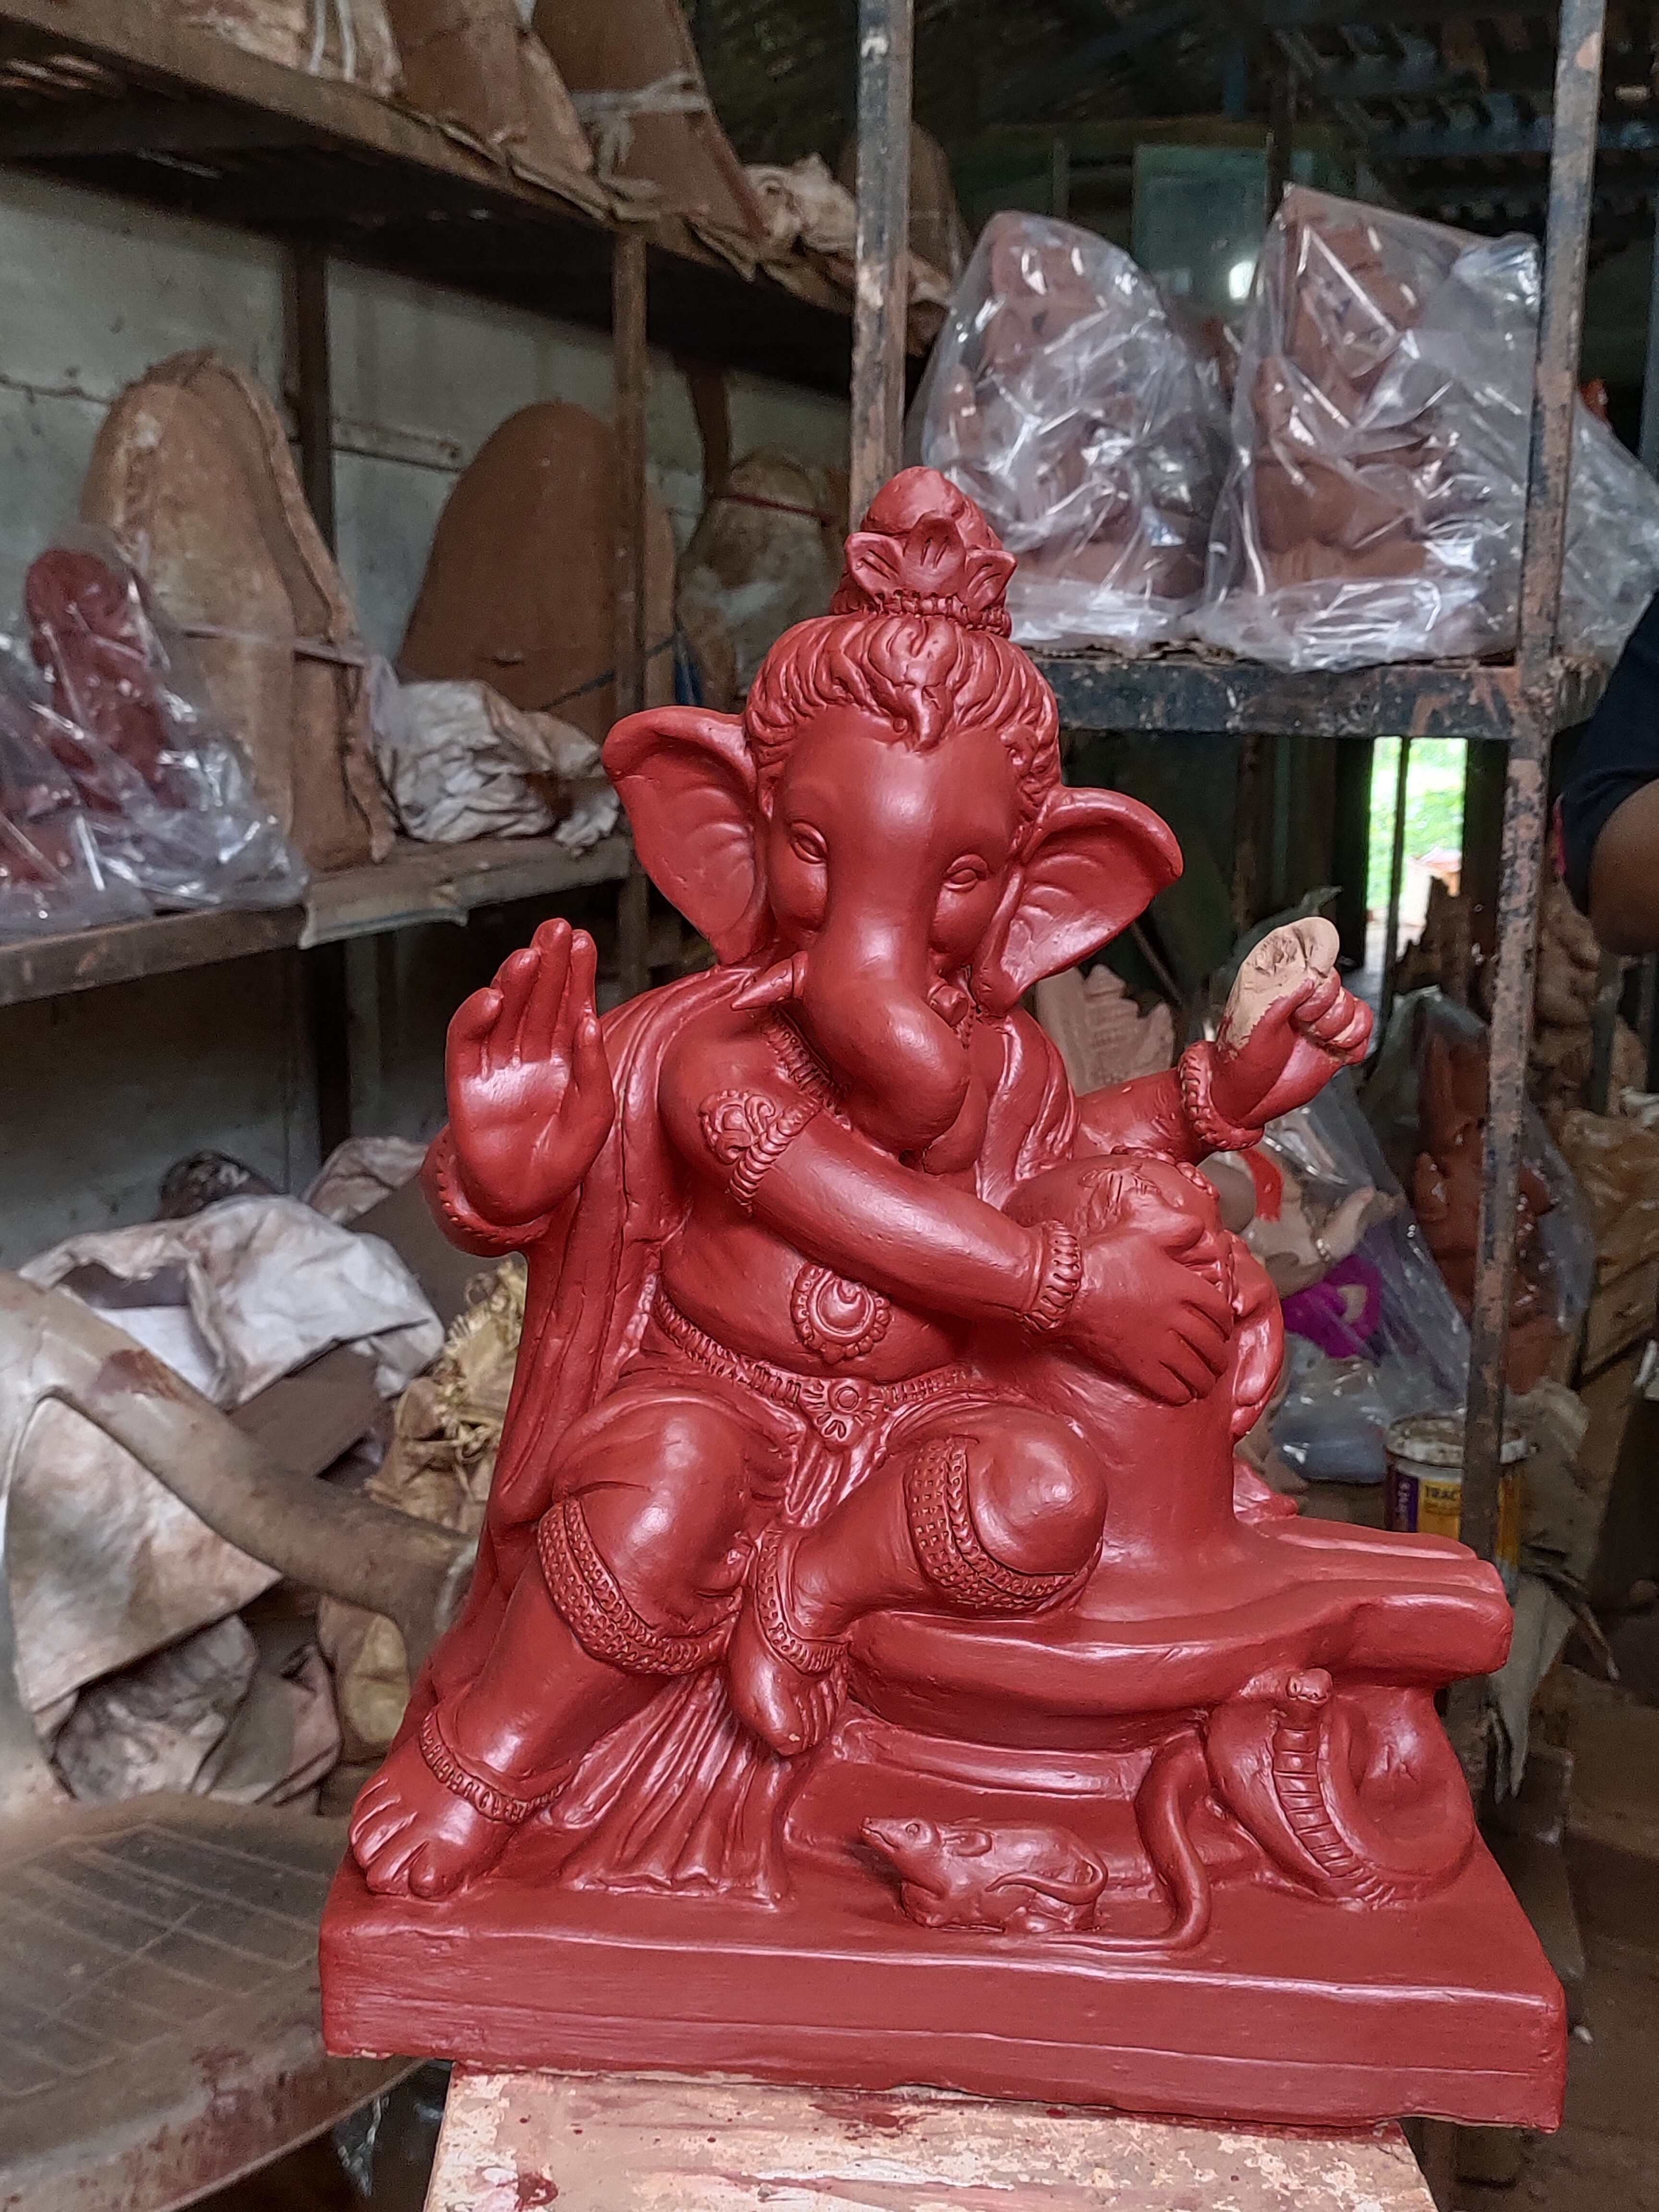
\includegraphics[width=\linewidth]{pottery2.jpg}
			\end{minipage}
			\vfill
			\begin{minipage}[c]{0.45\textwidth}
				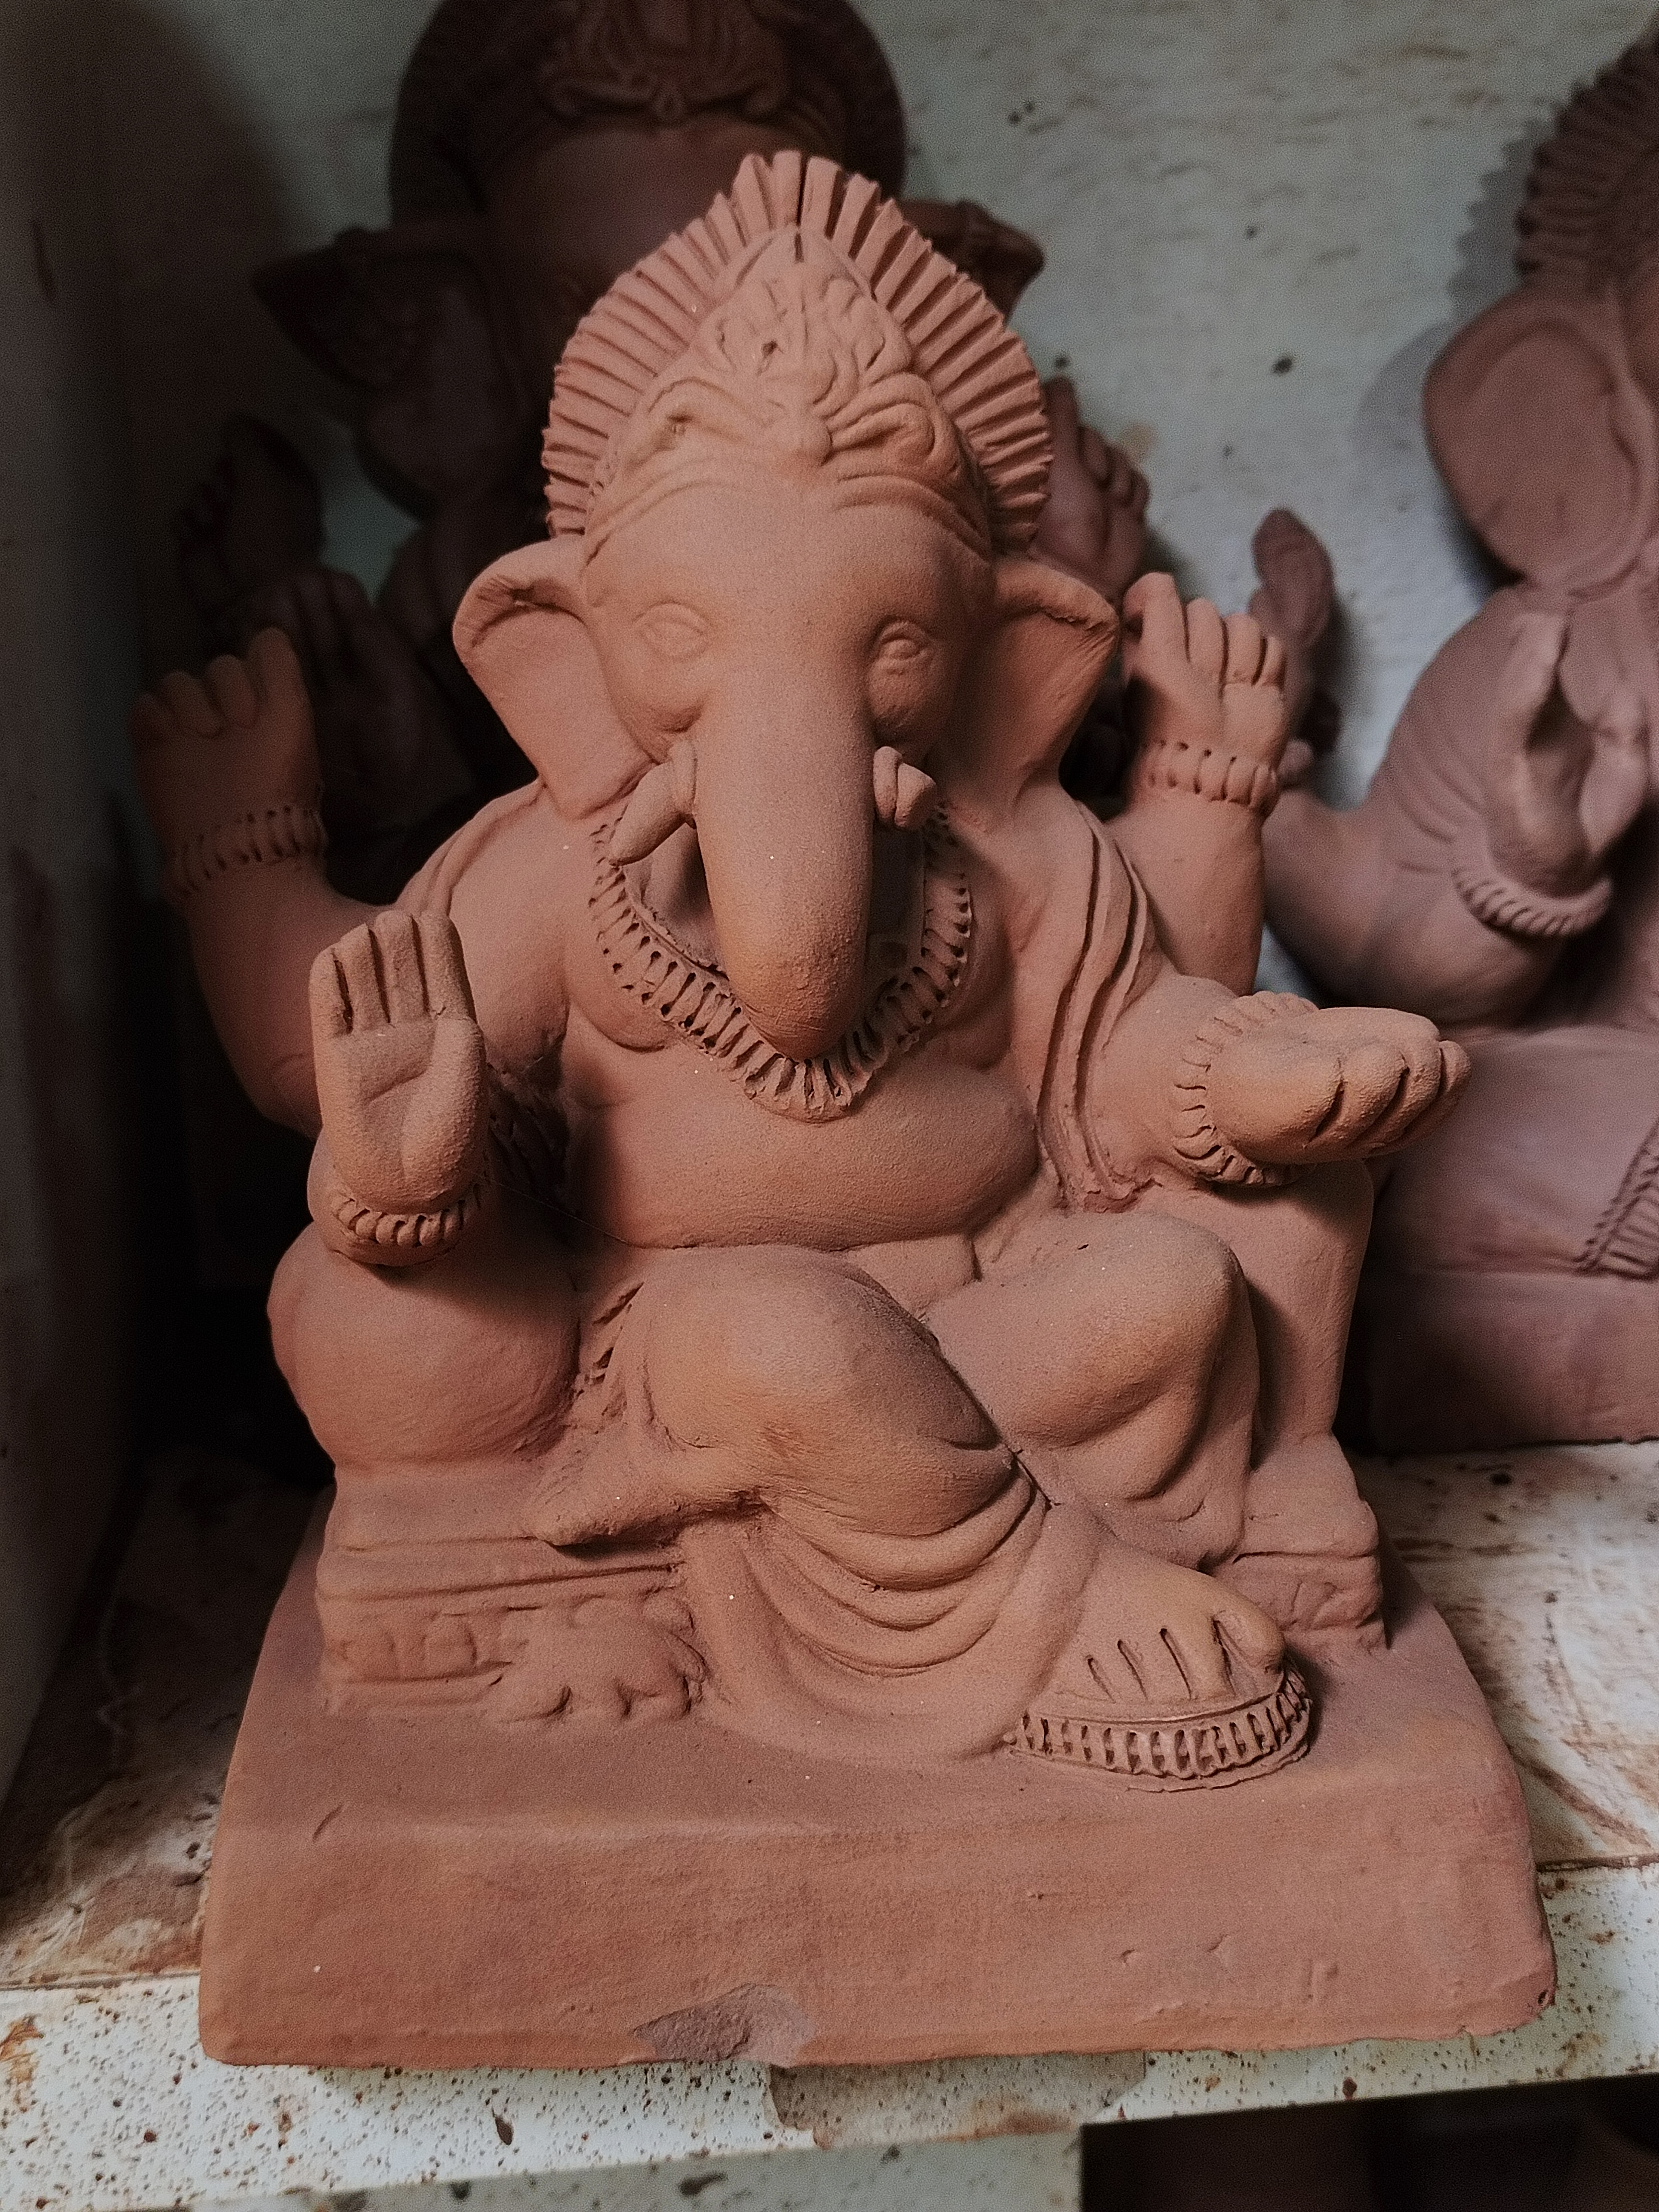
\includegraphics[width=\linewidth]{pottery3.jpg}
			\end{minipage}\hfill%
			\begin{minipage}[c]{0.45\textwidth}
				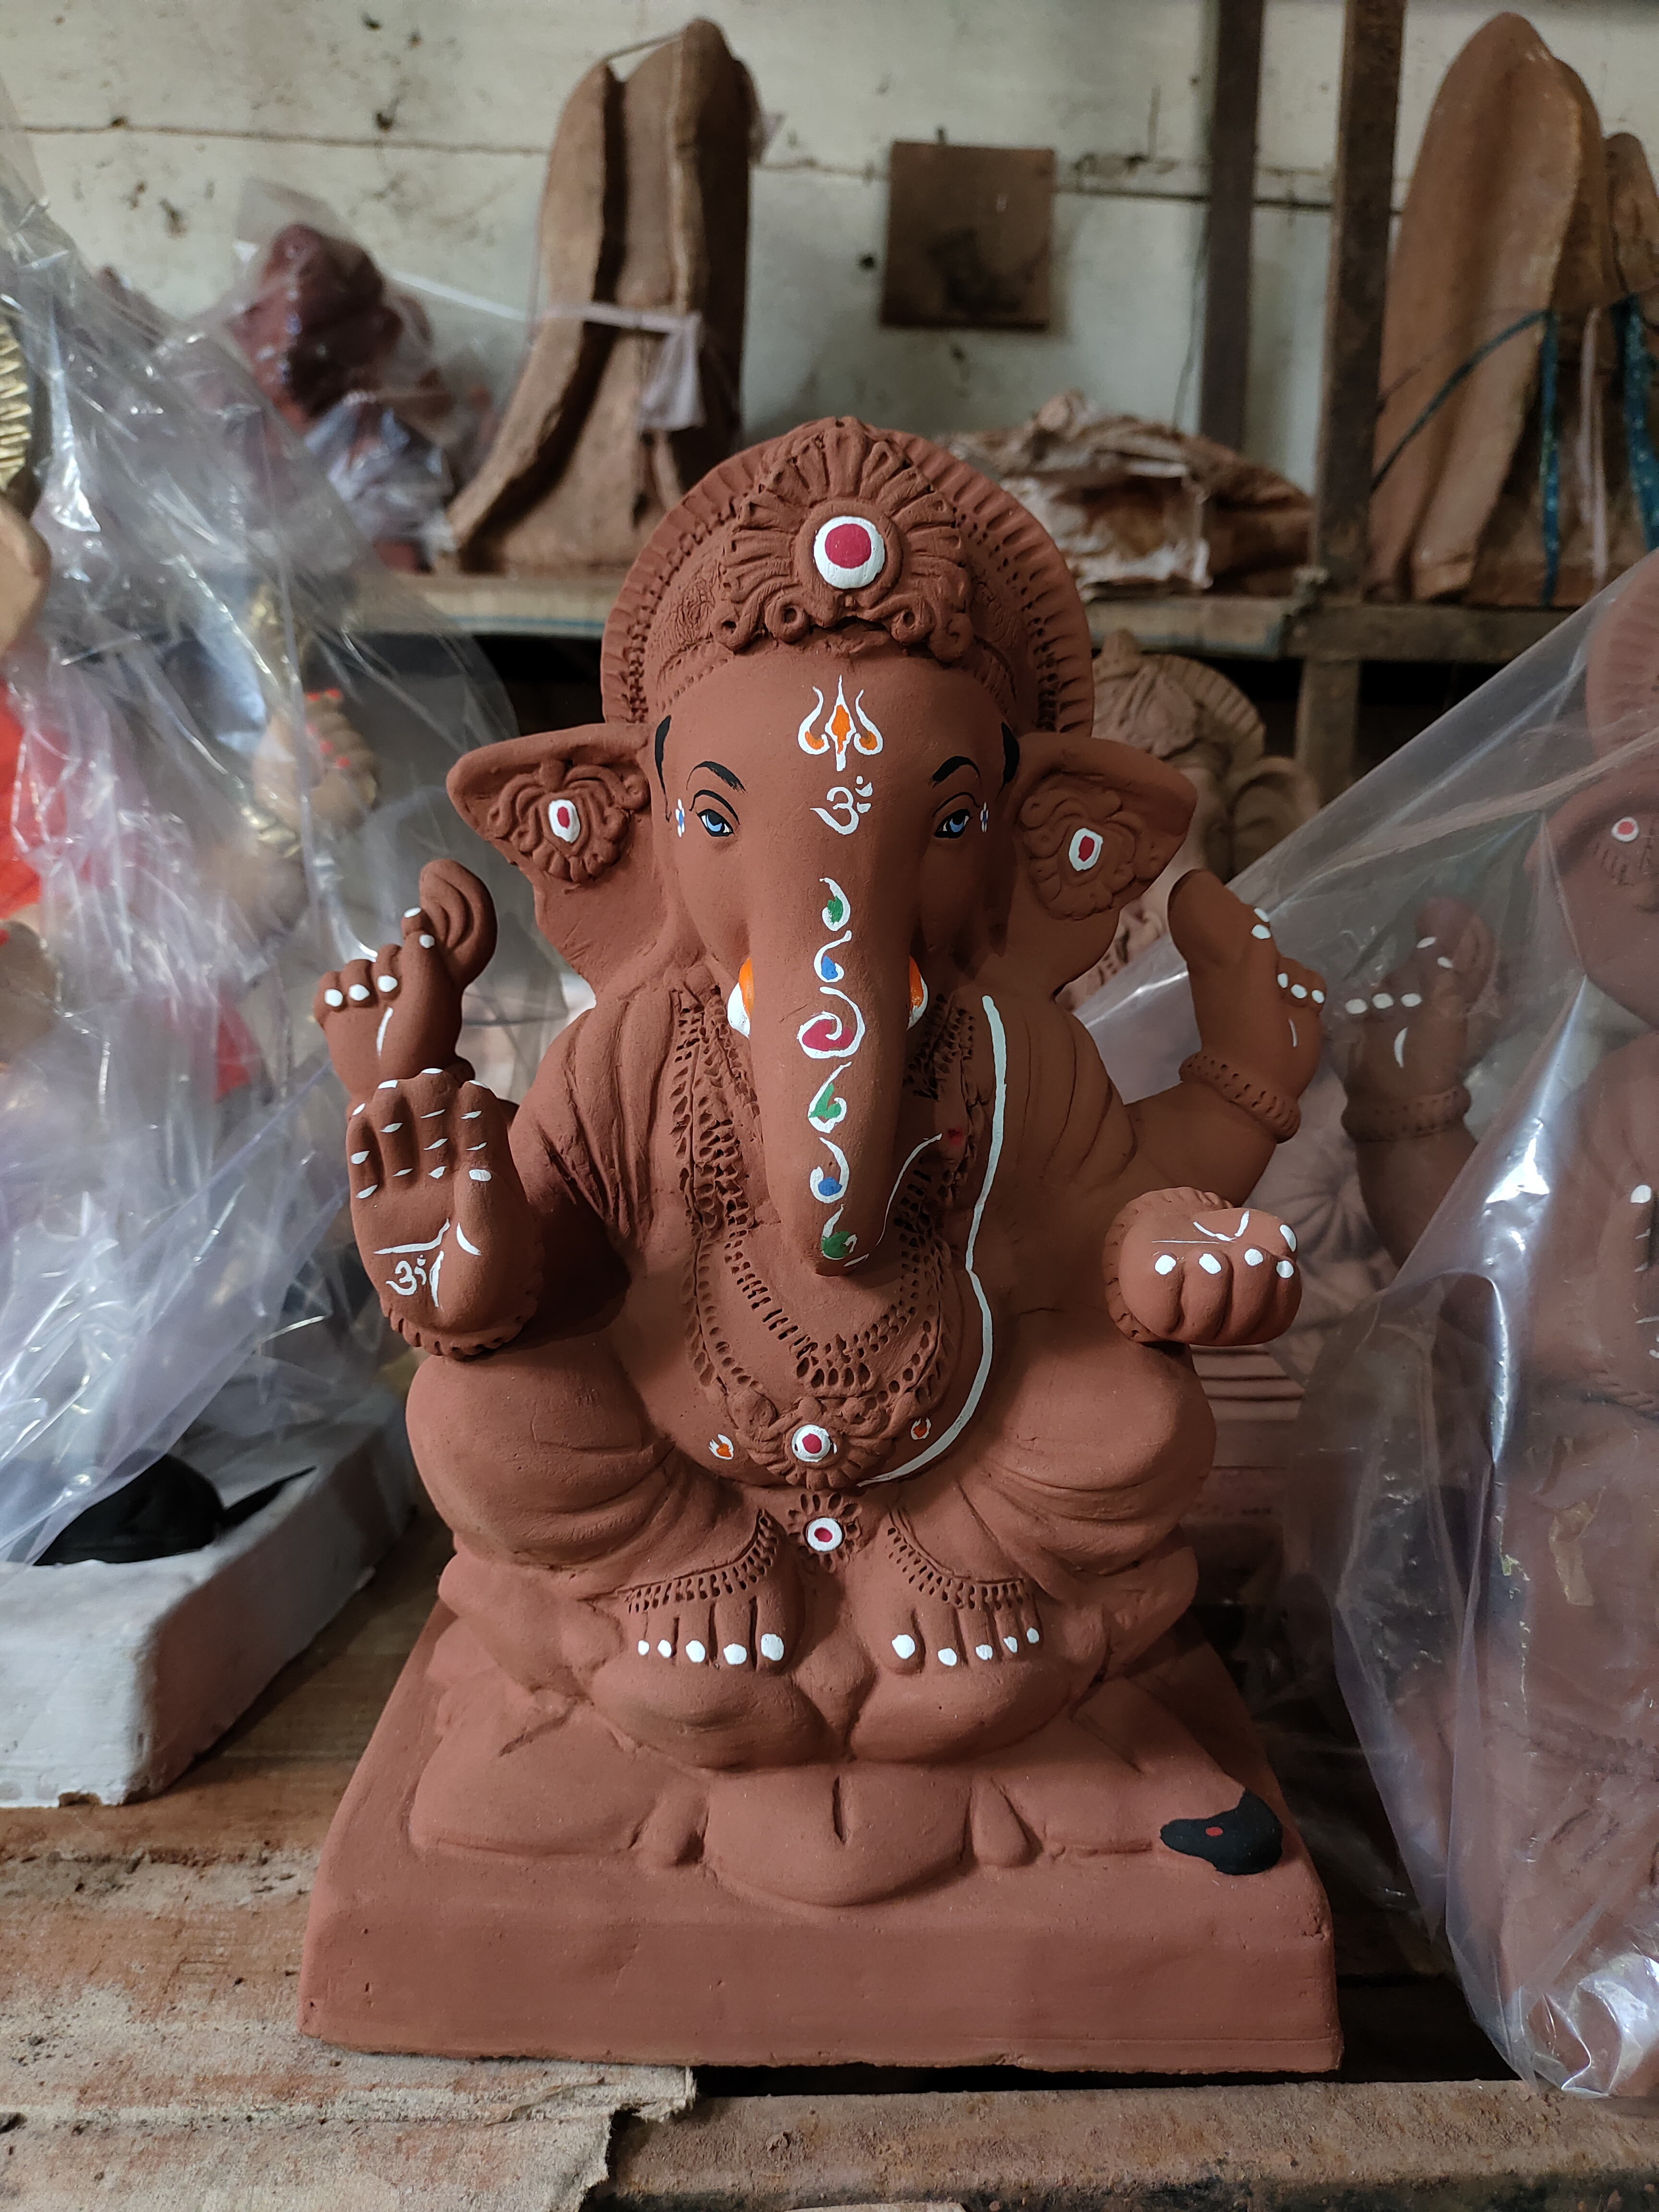
\includegraphics[width=\linewidth]{pottery4.jpg}
			\end{minipage}
			\vfill
		\end{center}
		
		\clearpage
		
		\begin{center}
			\begin{minipage}[c]{0.45\textwidth}
				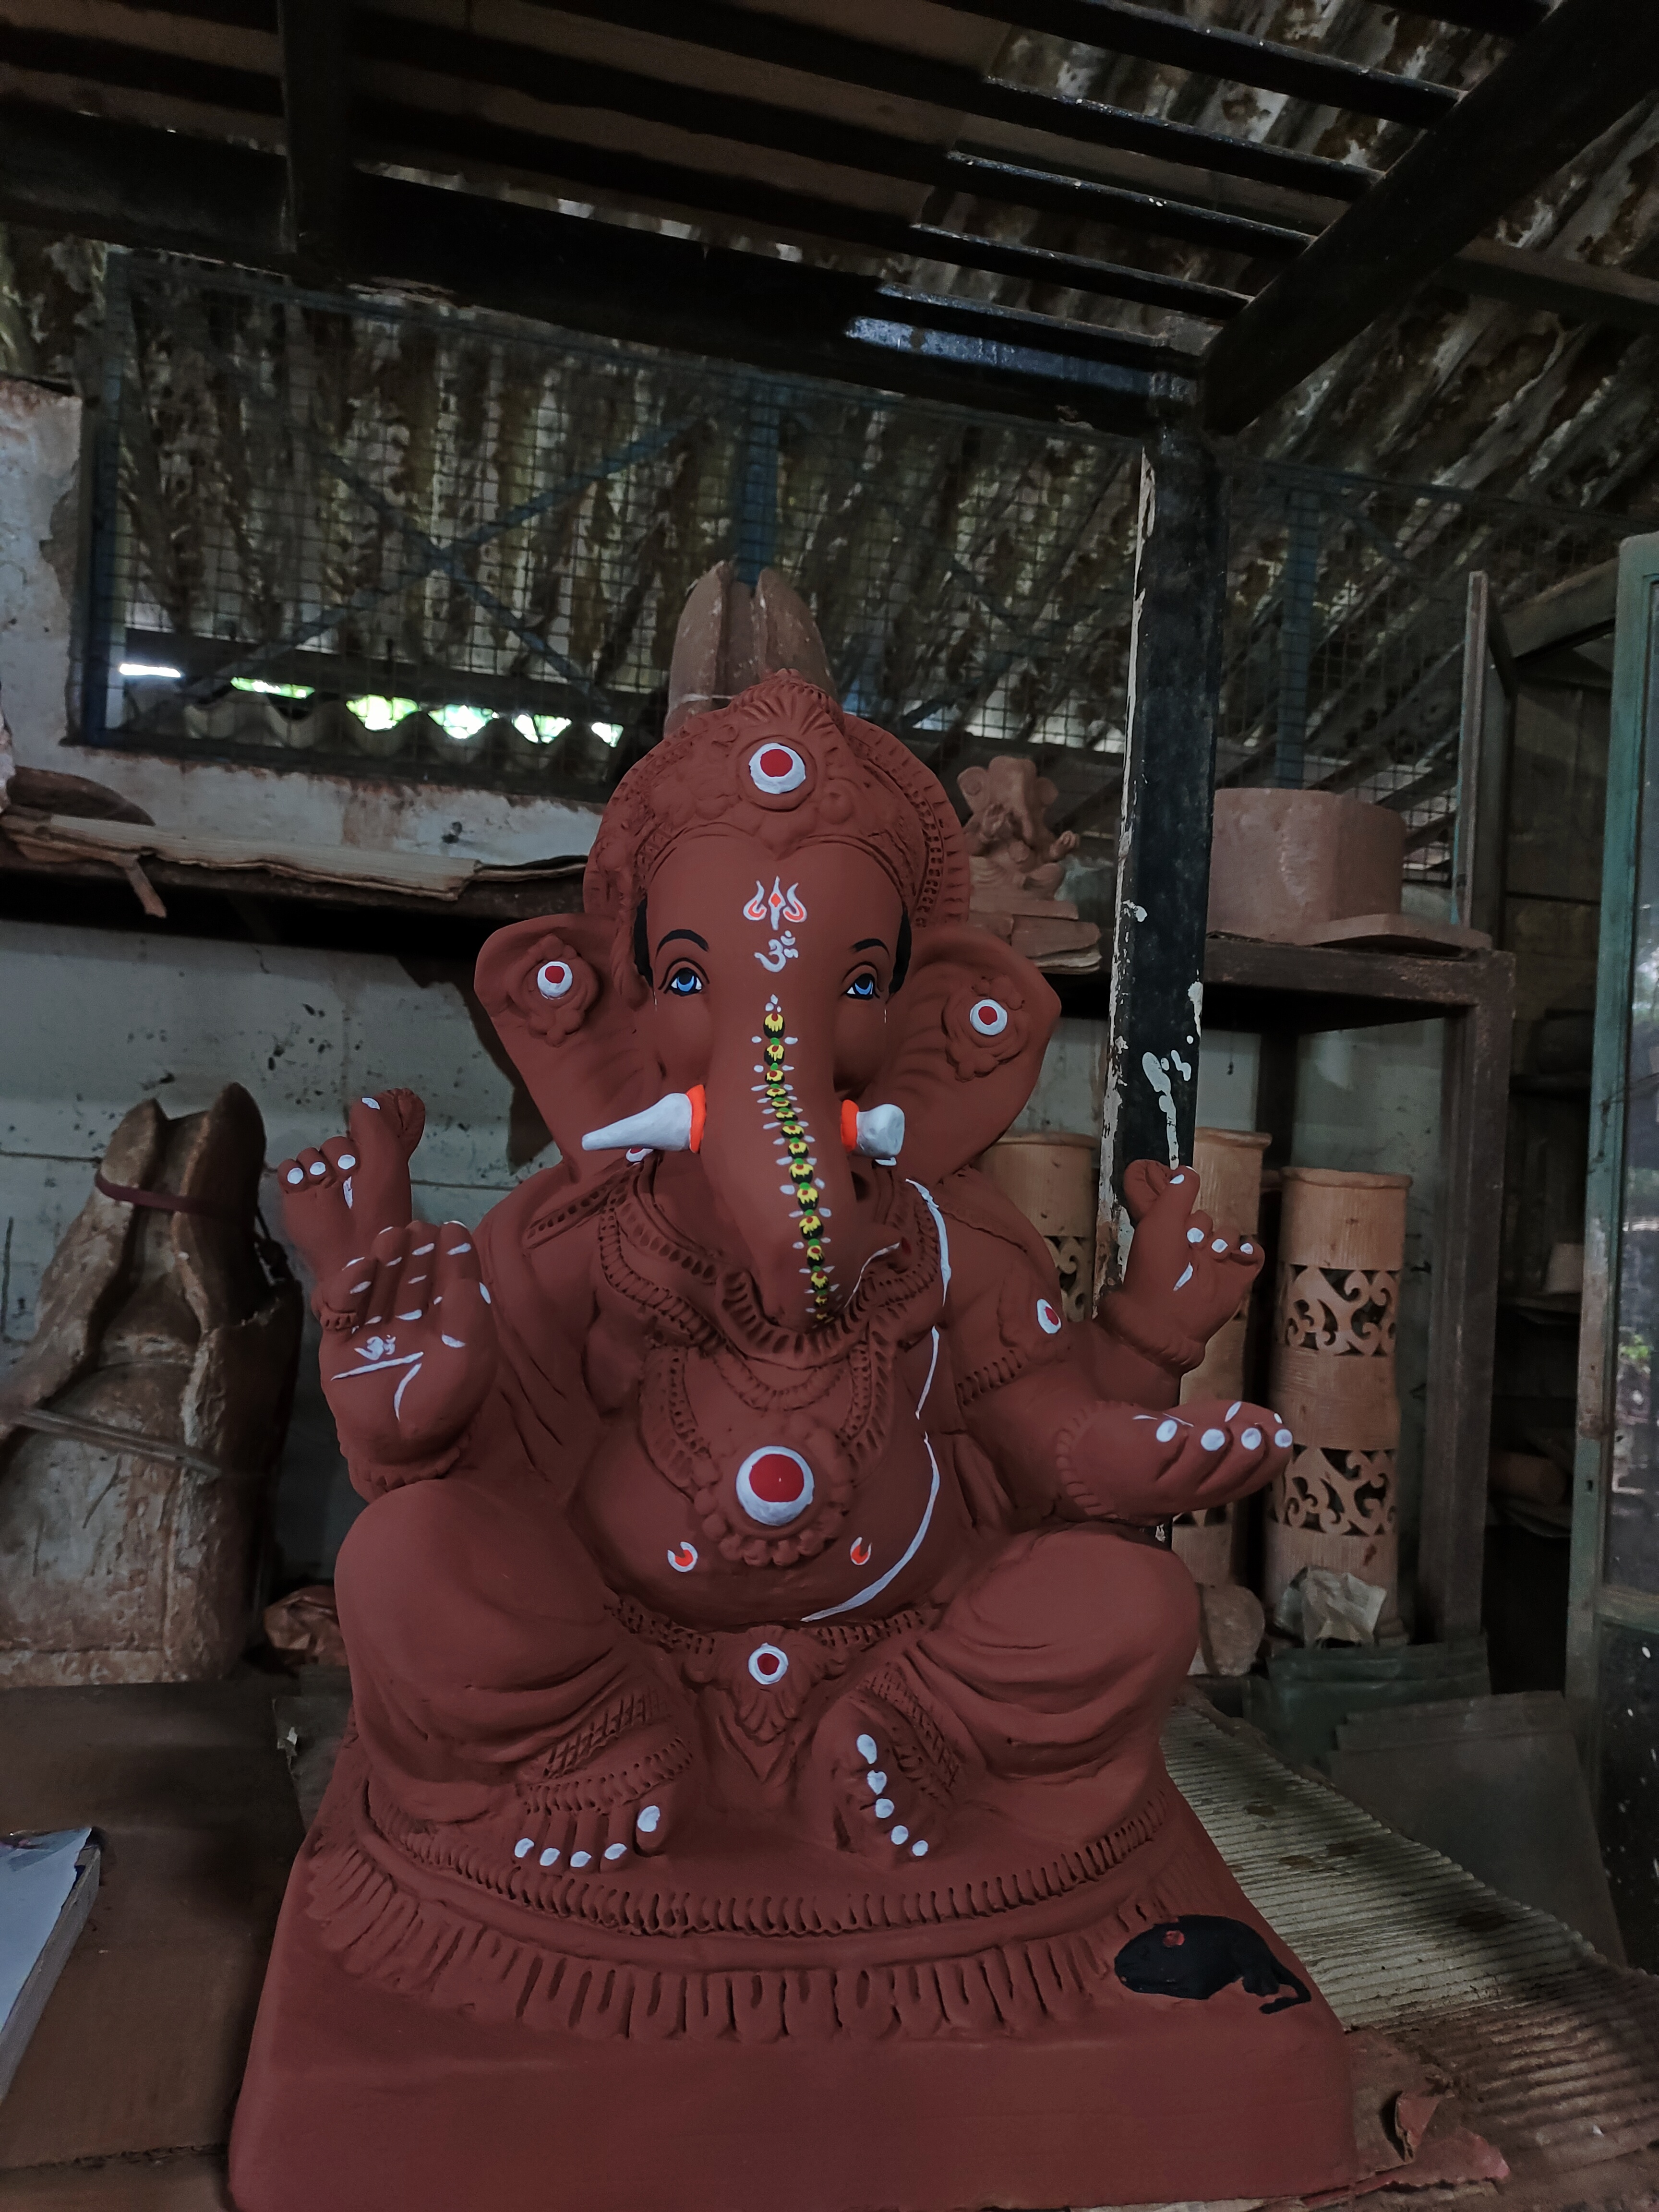
\includegraphics[width=\linewidth]{pottery5.jpg}
			\end{minipage}\hfill%
			\begin{minipage}[c]{0.45\textwidth}
				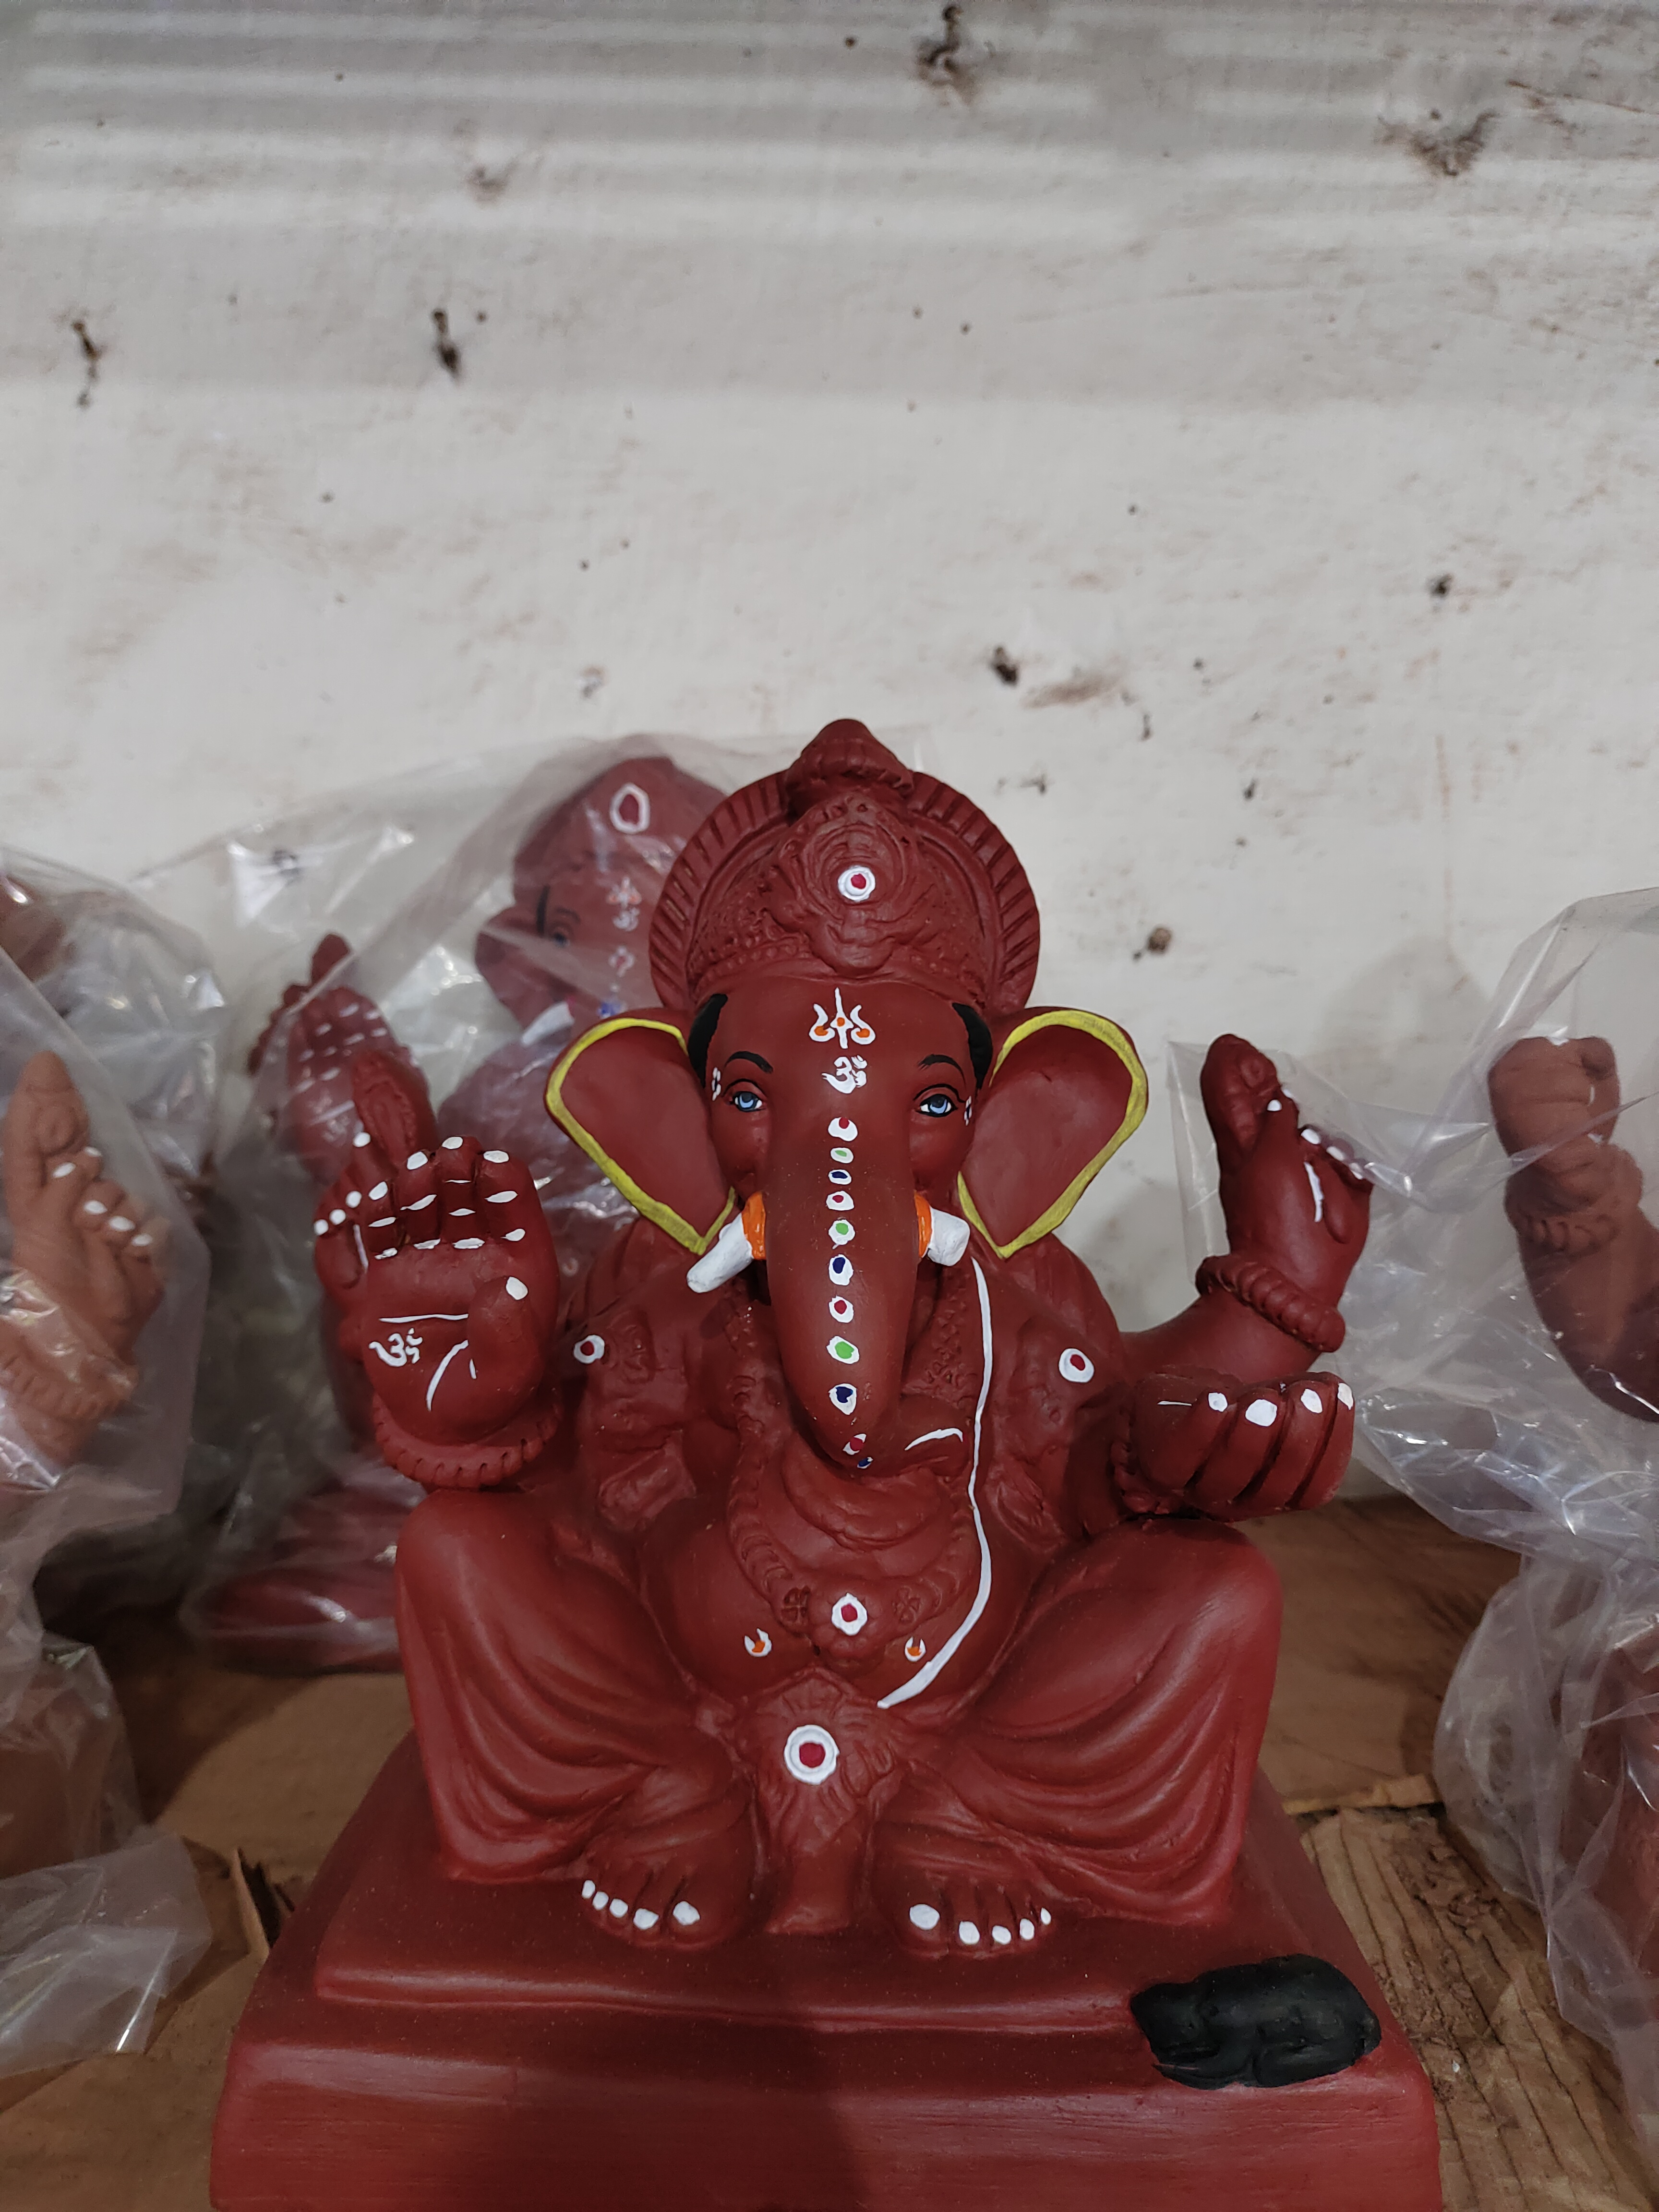
\includegraphics[width=\linewidth]{pottery6.jpg}
			\end{minipage}
		\end{center}
		
		\vspace*{1.5cm}
		
		\begin{center}
			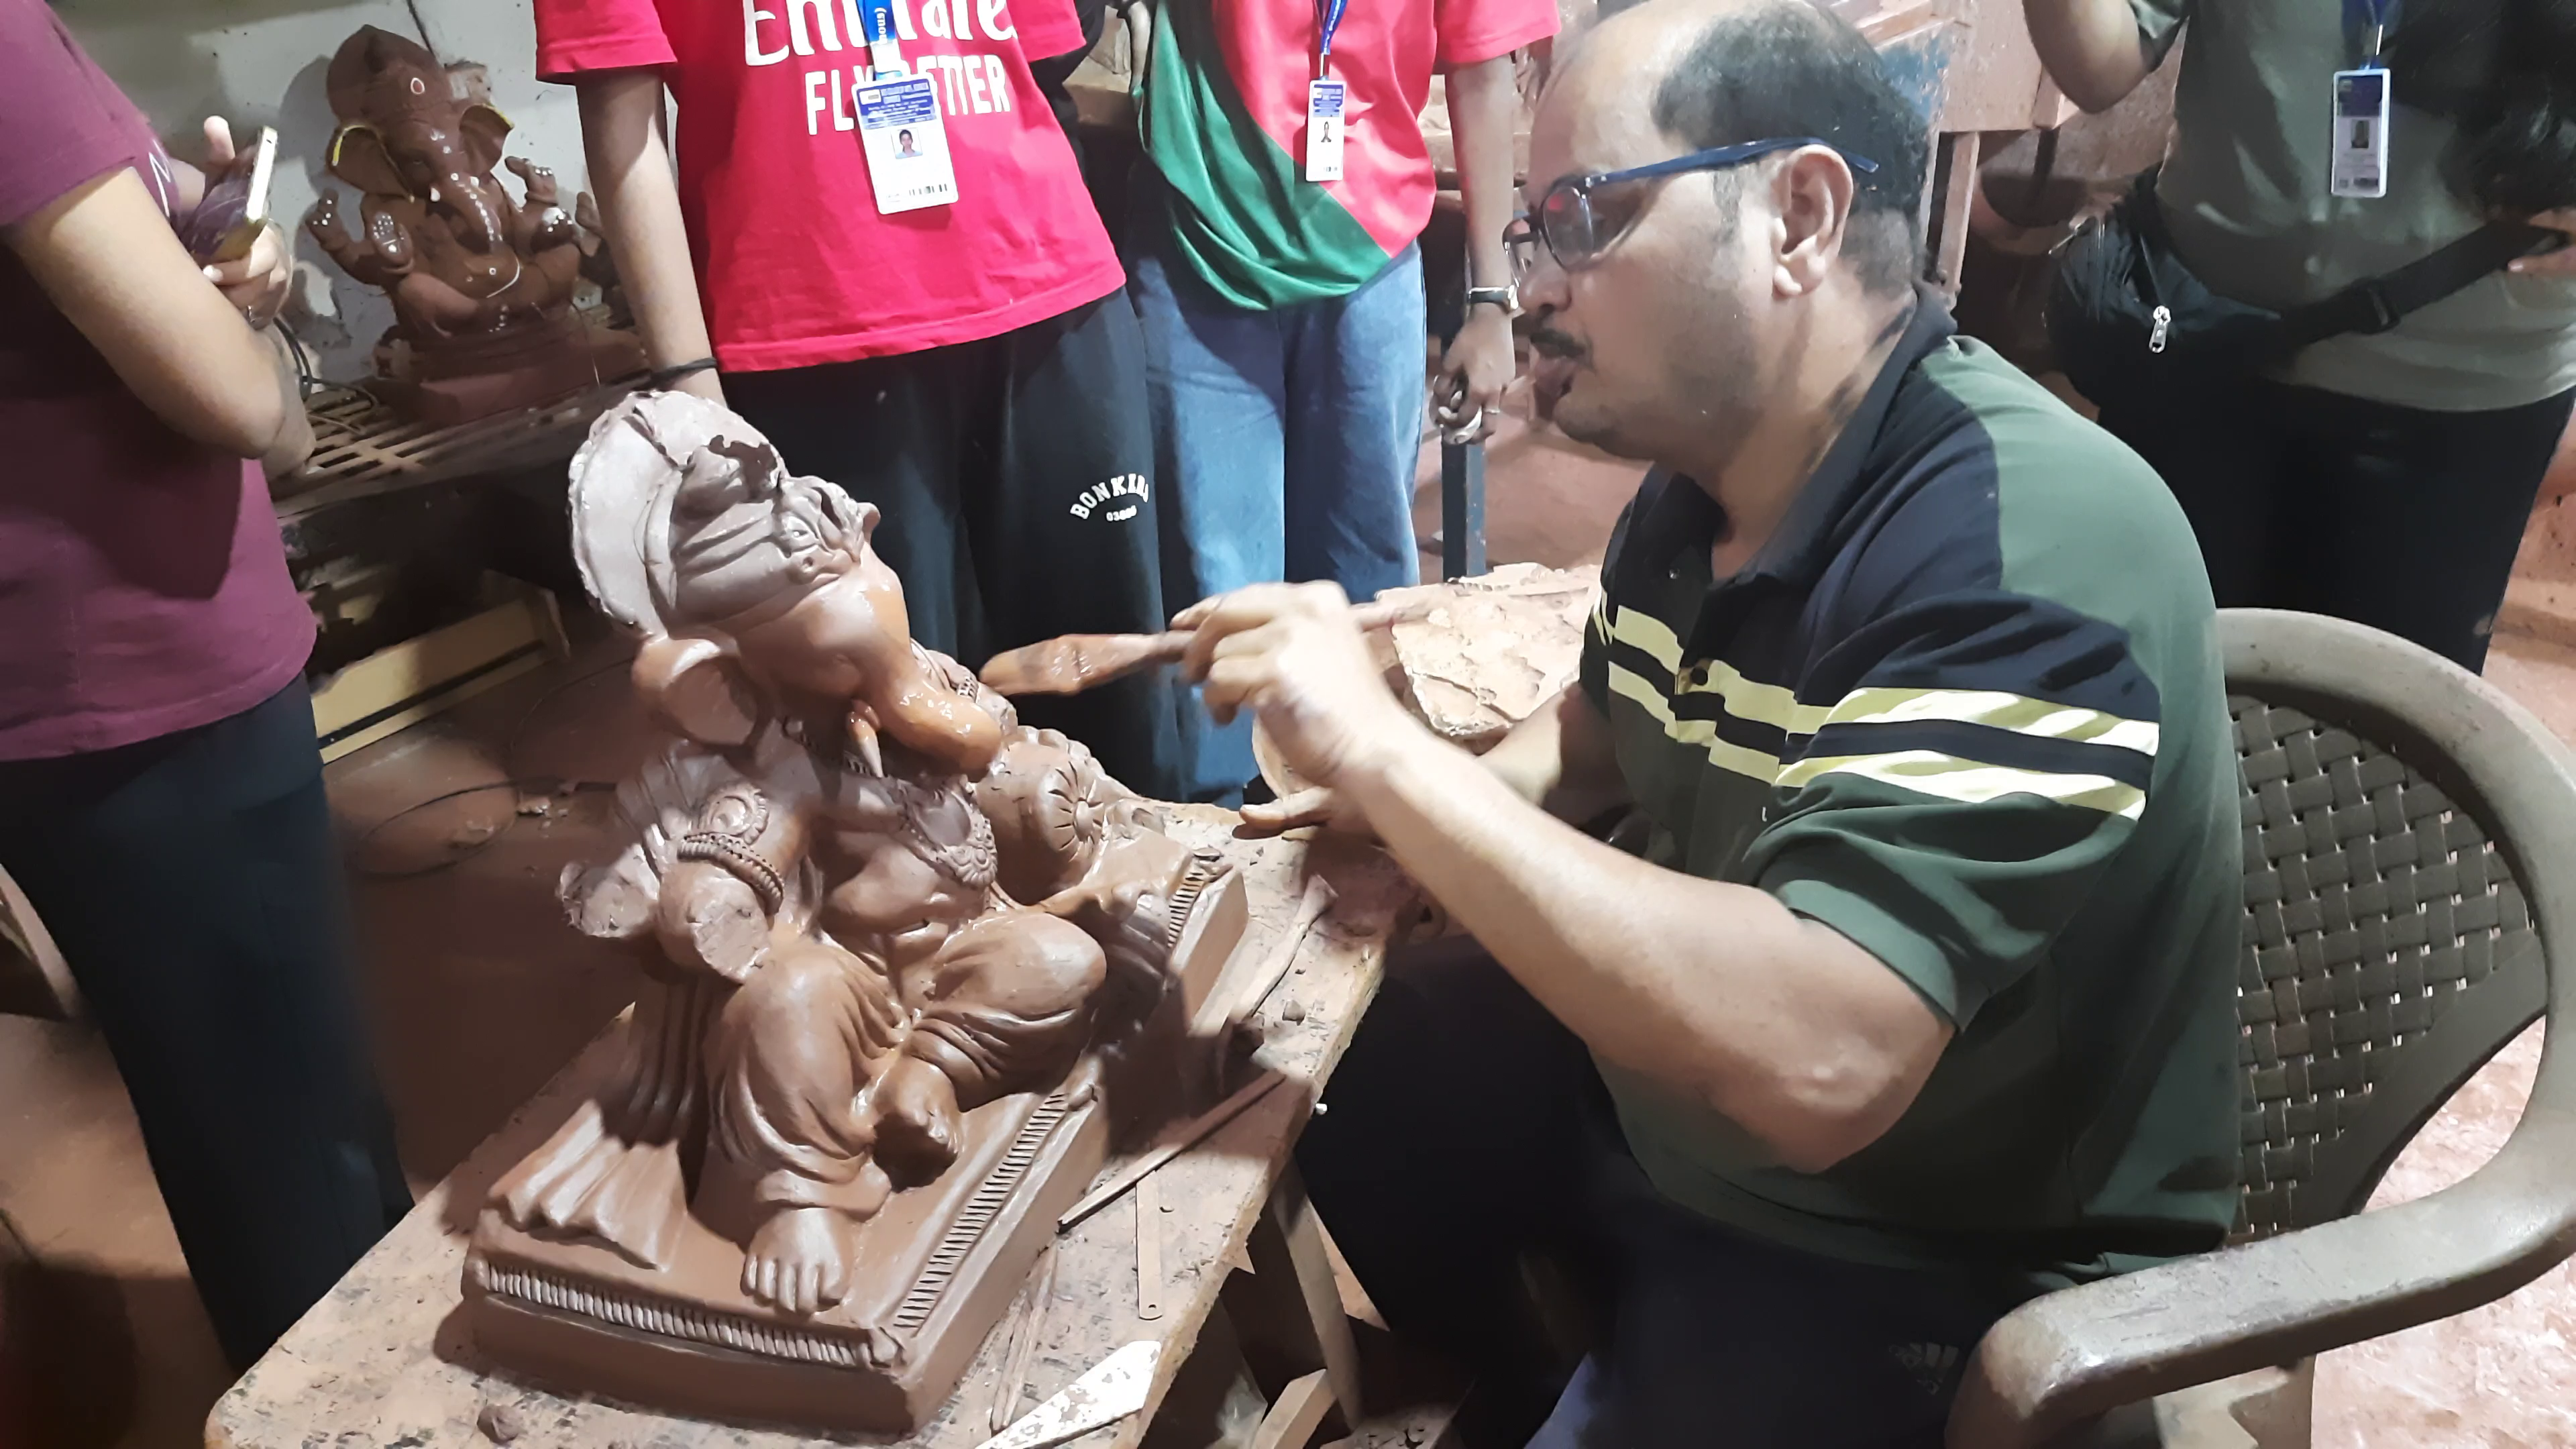
\includegraphics[width=\textwidth]{pottery7.png}
			\captionof{figure}{Clay idol crafting in progress for the upcoming Ganesh Chaturthi.}
		\end{center}
		
		\clearpage
		
		\begin{center}
			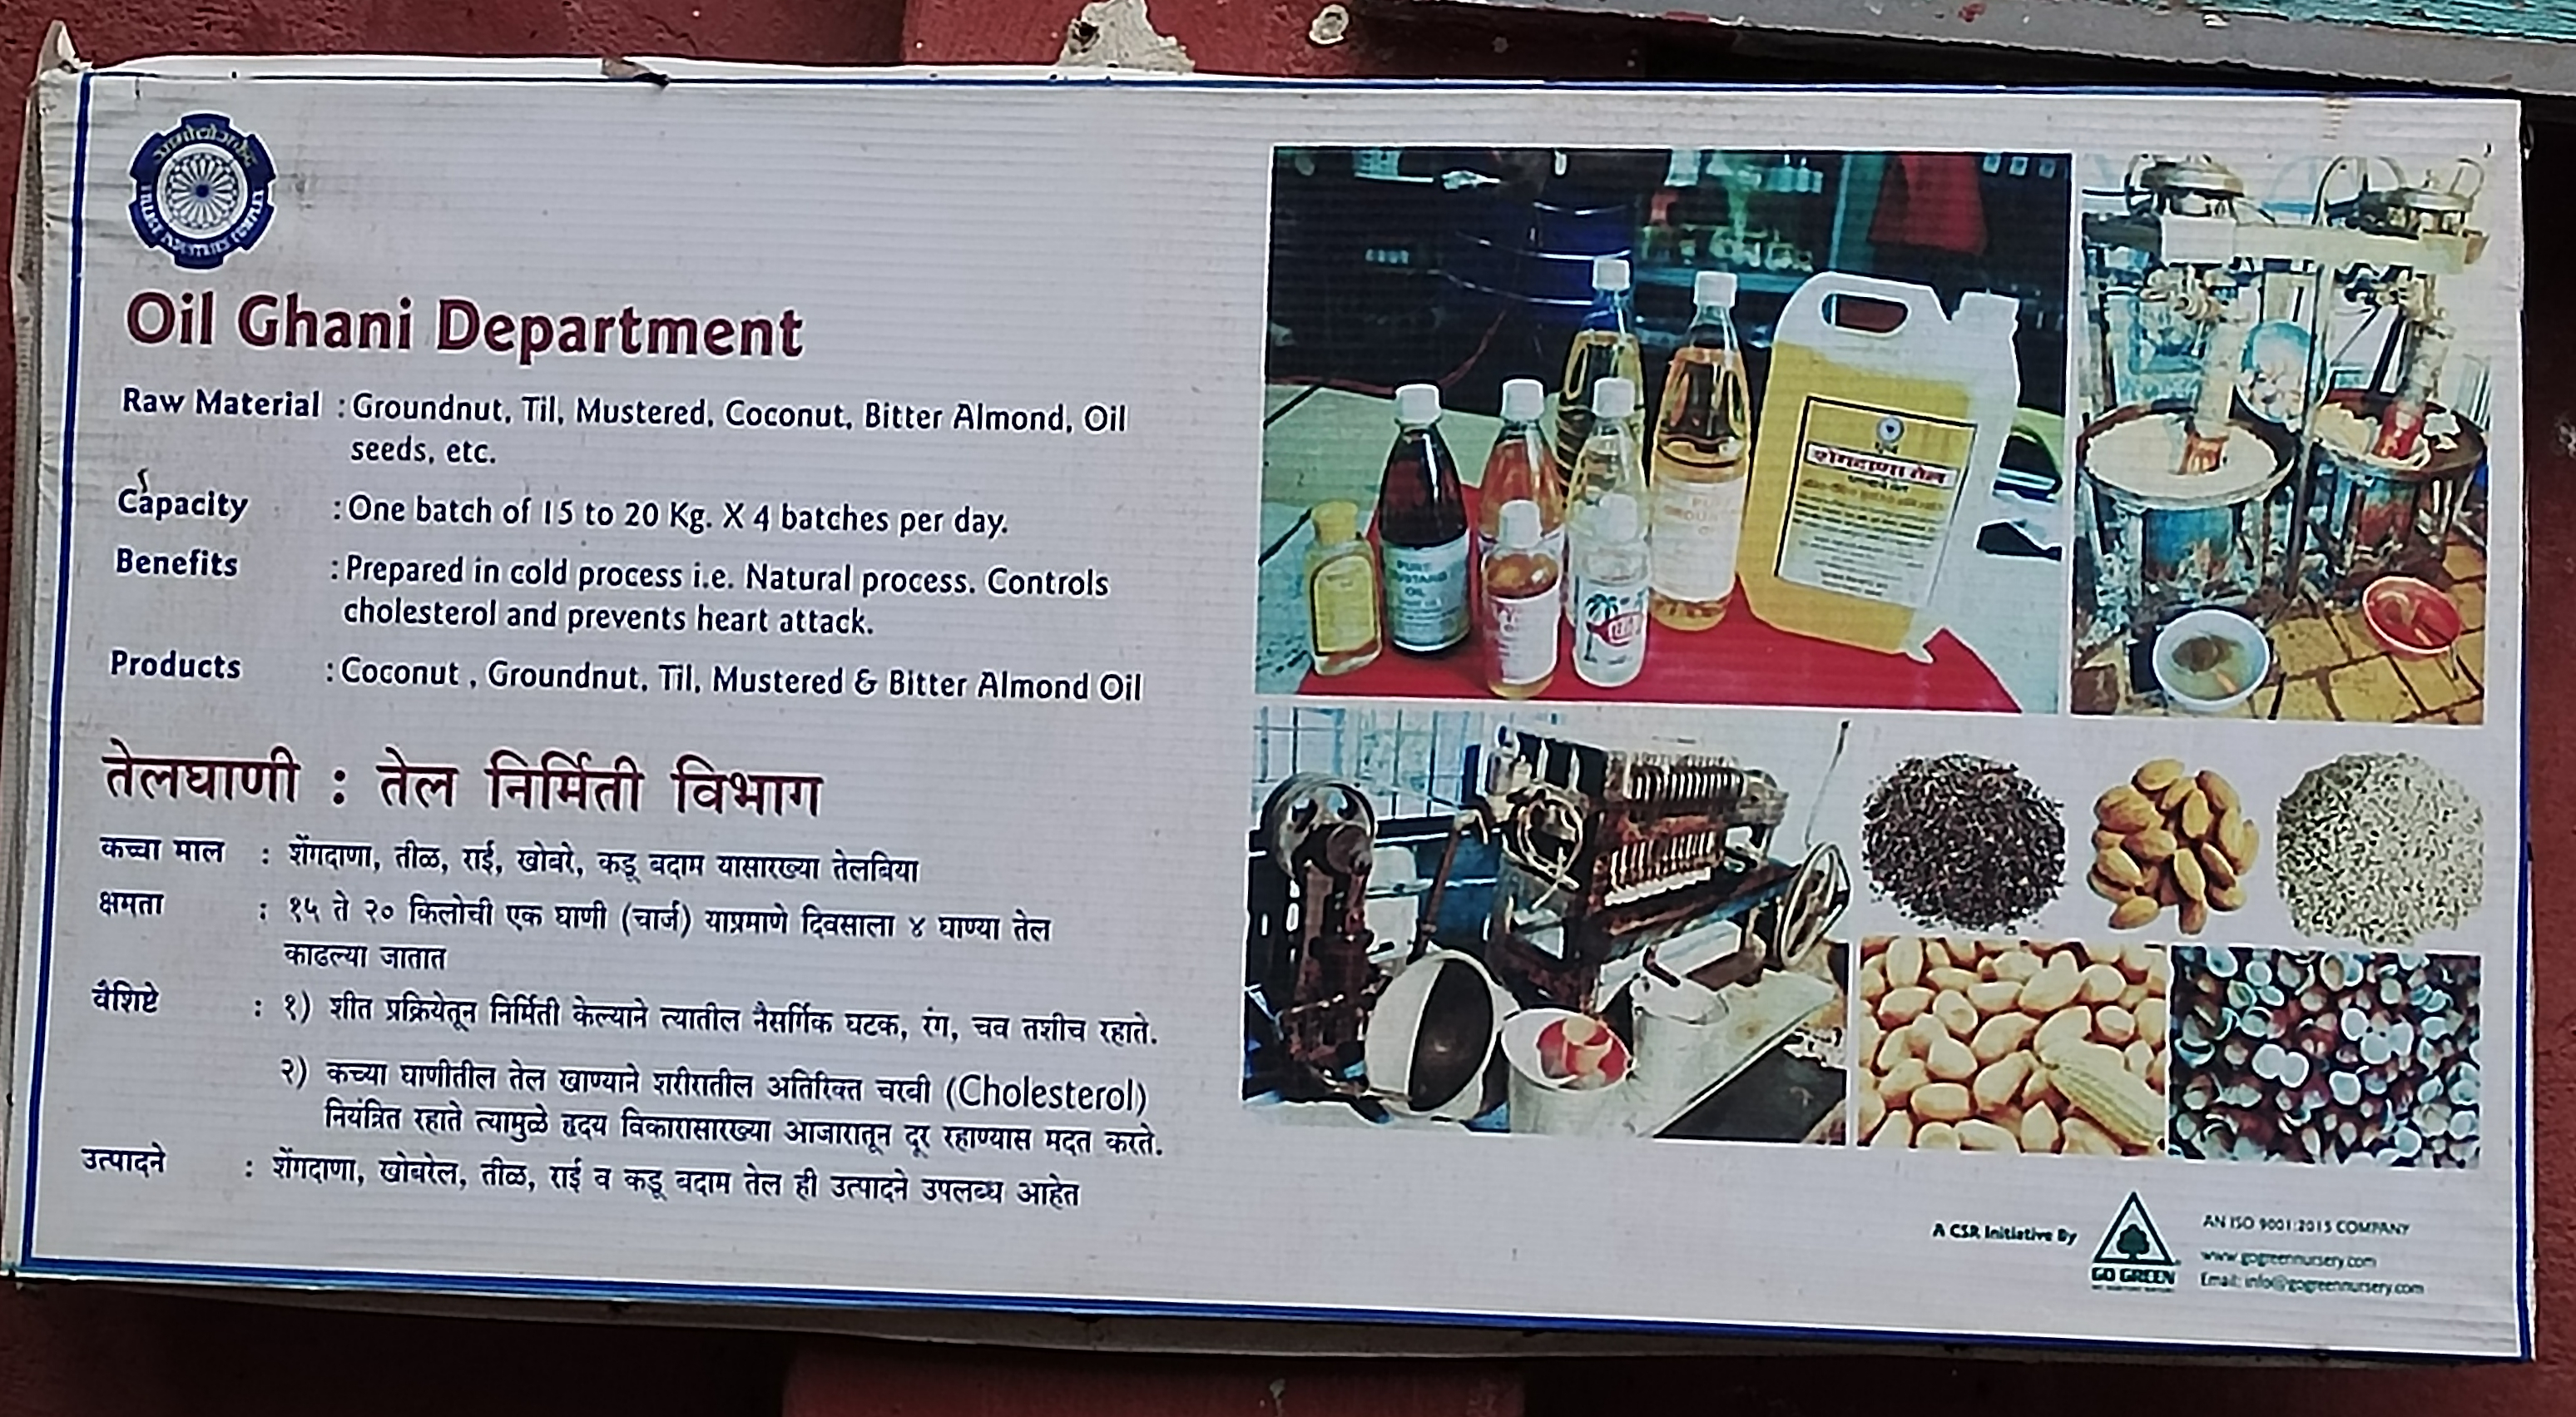
\includegraphics[width=\textwidth]{oil1.jpg}
			
			\vspace*{1.5cm}
			
			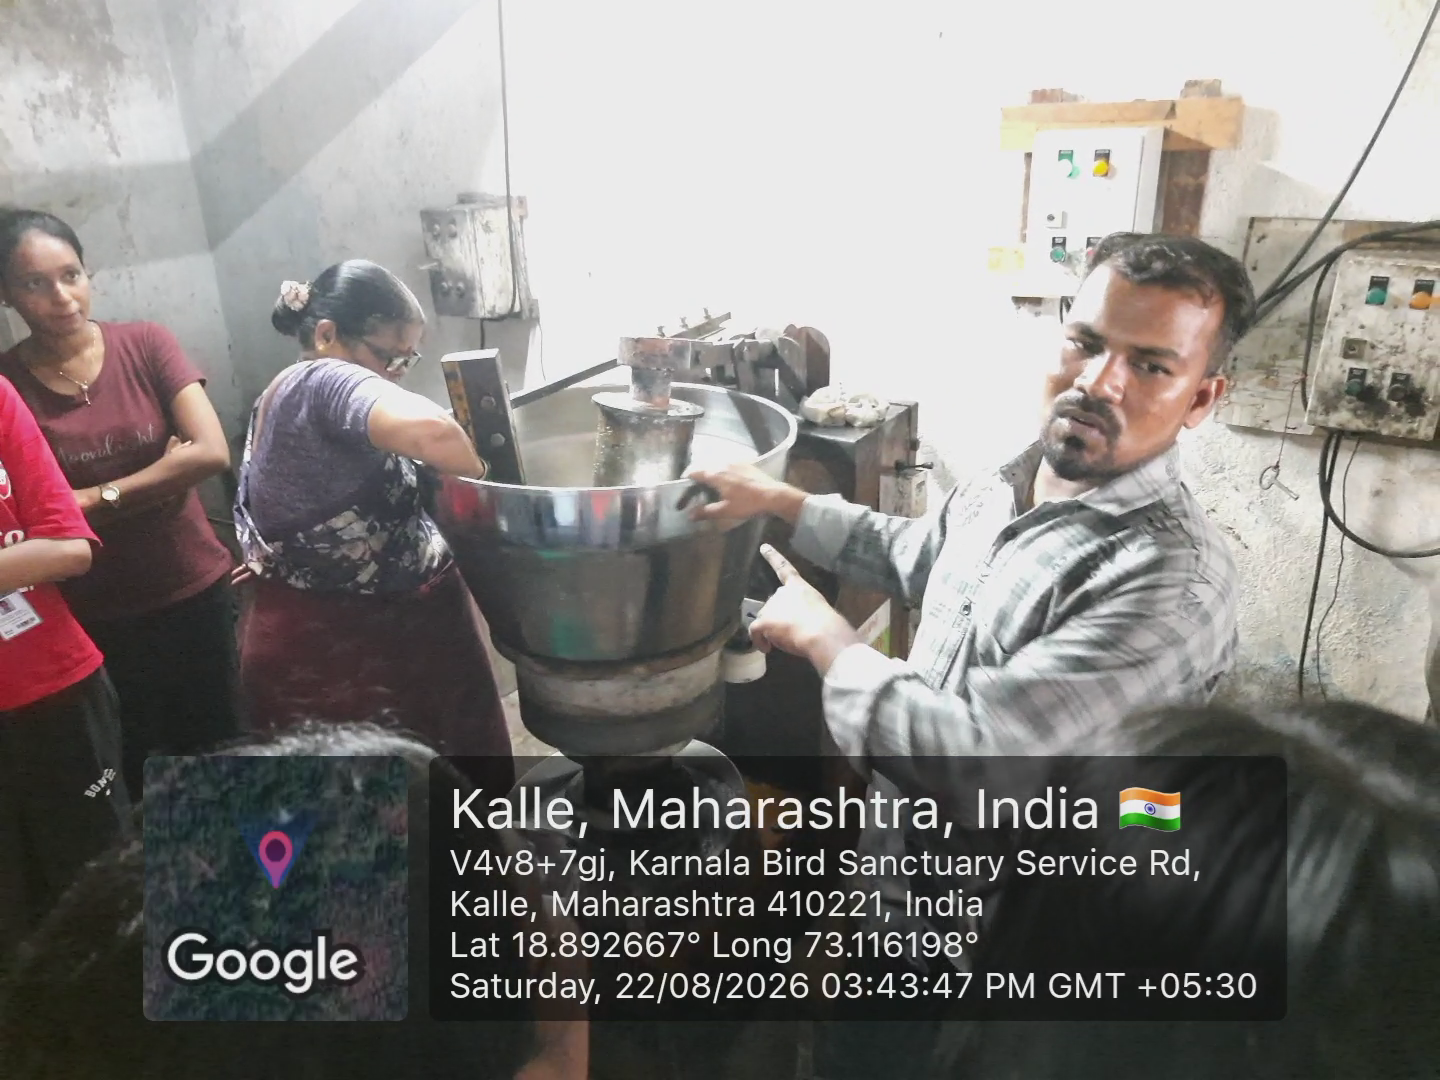
\includegraphics[width=\textwidth]{oil3.png}
			\captionof{figure}[Coconut oil extraction]{Demonstration of how coconut oil is obtained from coldpress.}
		\end{center}
		
		\clearpage
		
		\topskip0pt
		\vspace*{\fill}
		\begin{center}
			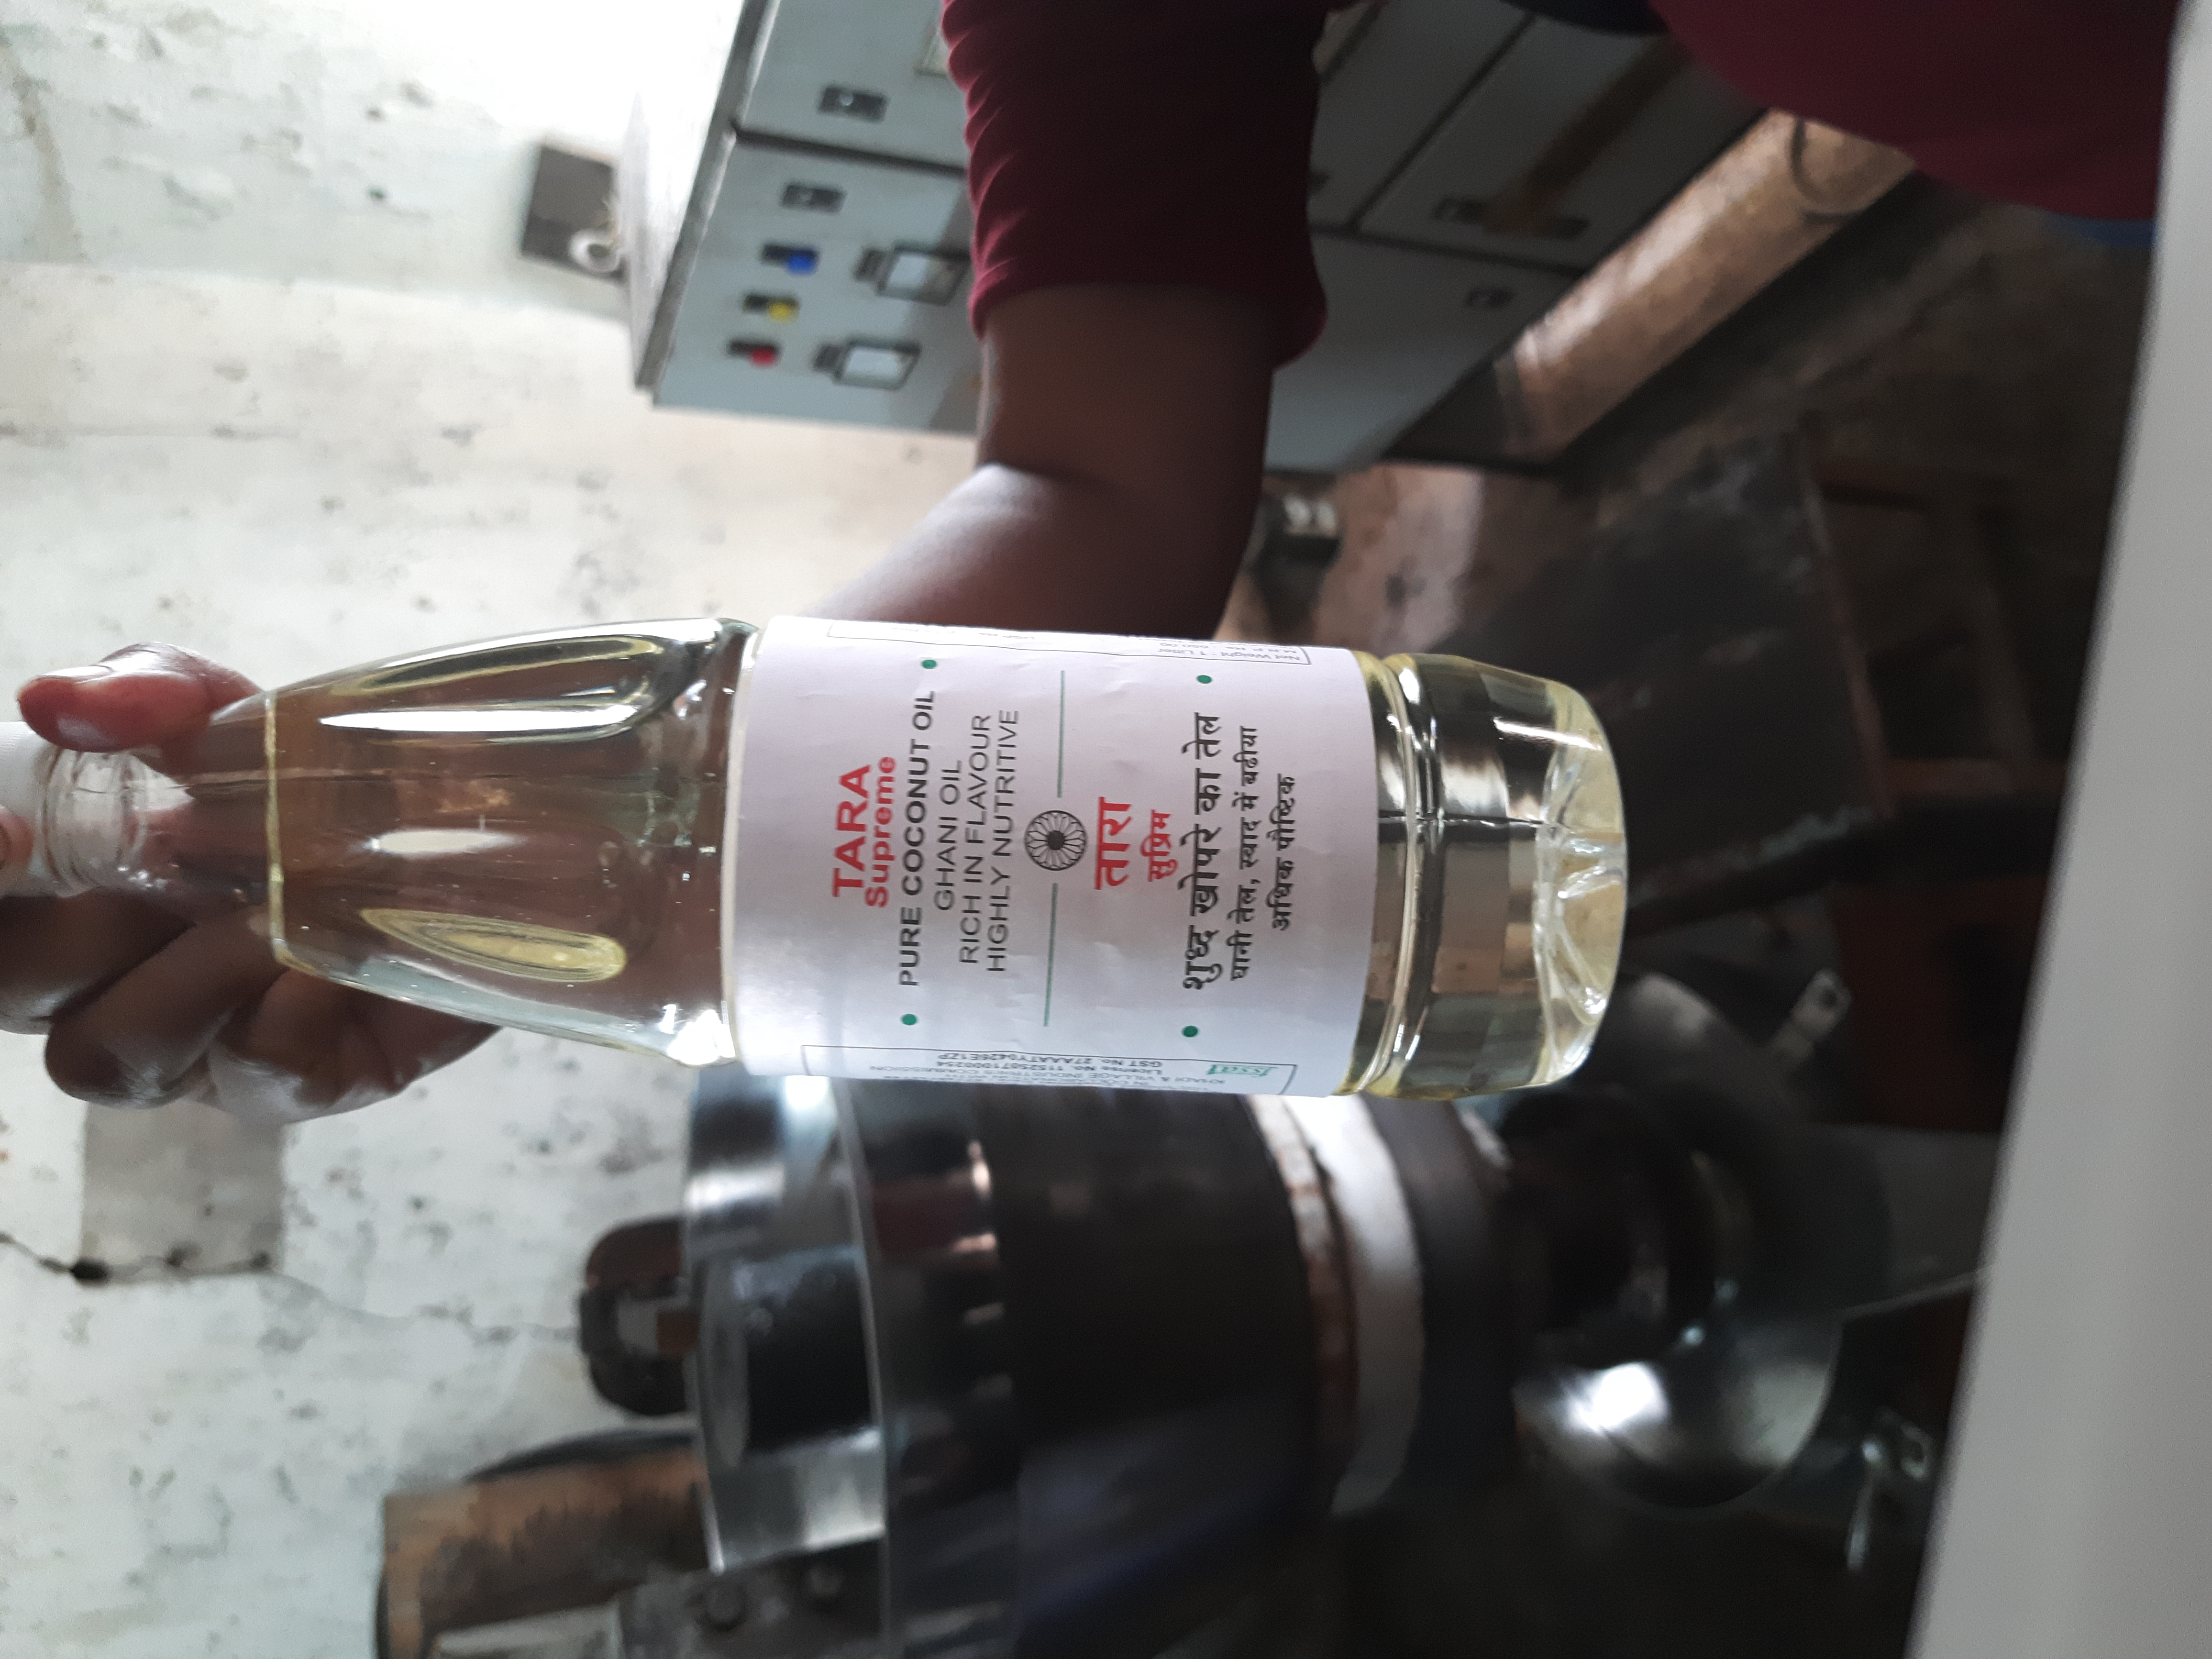
\includegraphics[width=\textwidth, angle=-90]{oil2.jpg}
			\captionof{figure}[Finished coconut oil]{\protect Finished product. The light colour is due to the absence of any preservatives. Expiry date is only six months from the date of manufacture due to the same reason.}
		\end{center}
		\vspace*{\fill}
		
		\clearpage
		
		\begin{center}
			\includegraphics[width=0.9\textwidth]{ymc1.jpg}
			\vfill
			\includegraphics[width=0.9\textwidth]{ymc2.jpg}
		\end{center}
		
		\clearpage
		
		\topskip0pt
		\vspace*{\fill}
		\begin{center}
			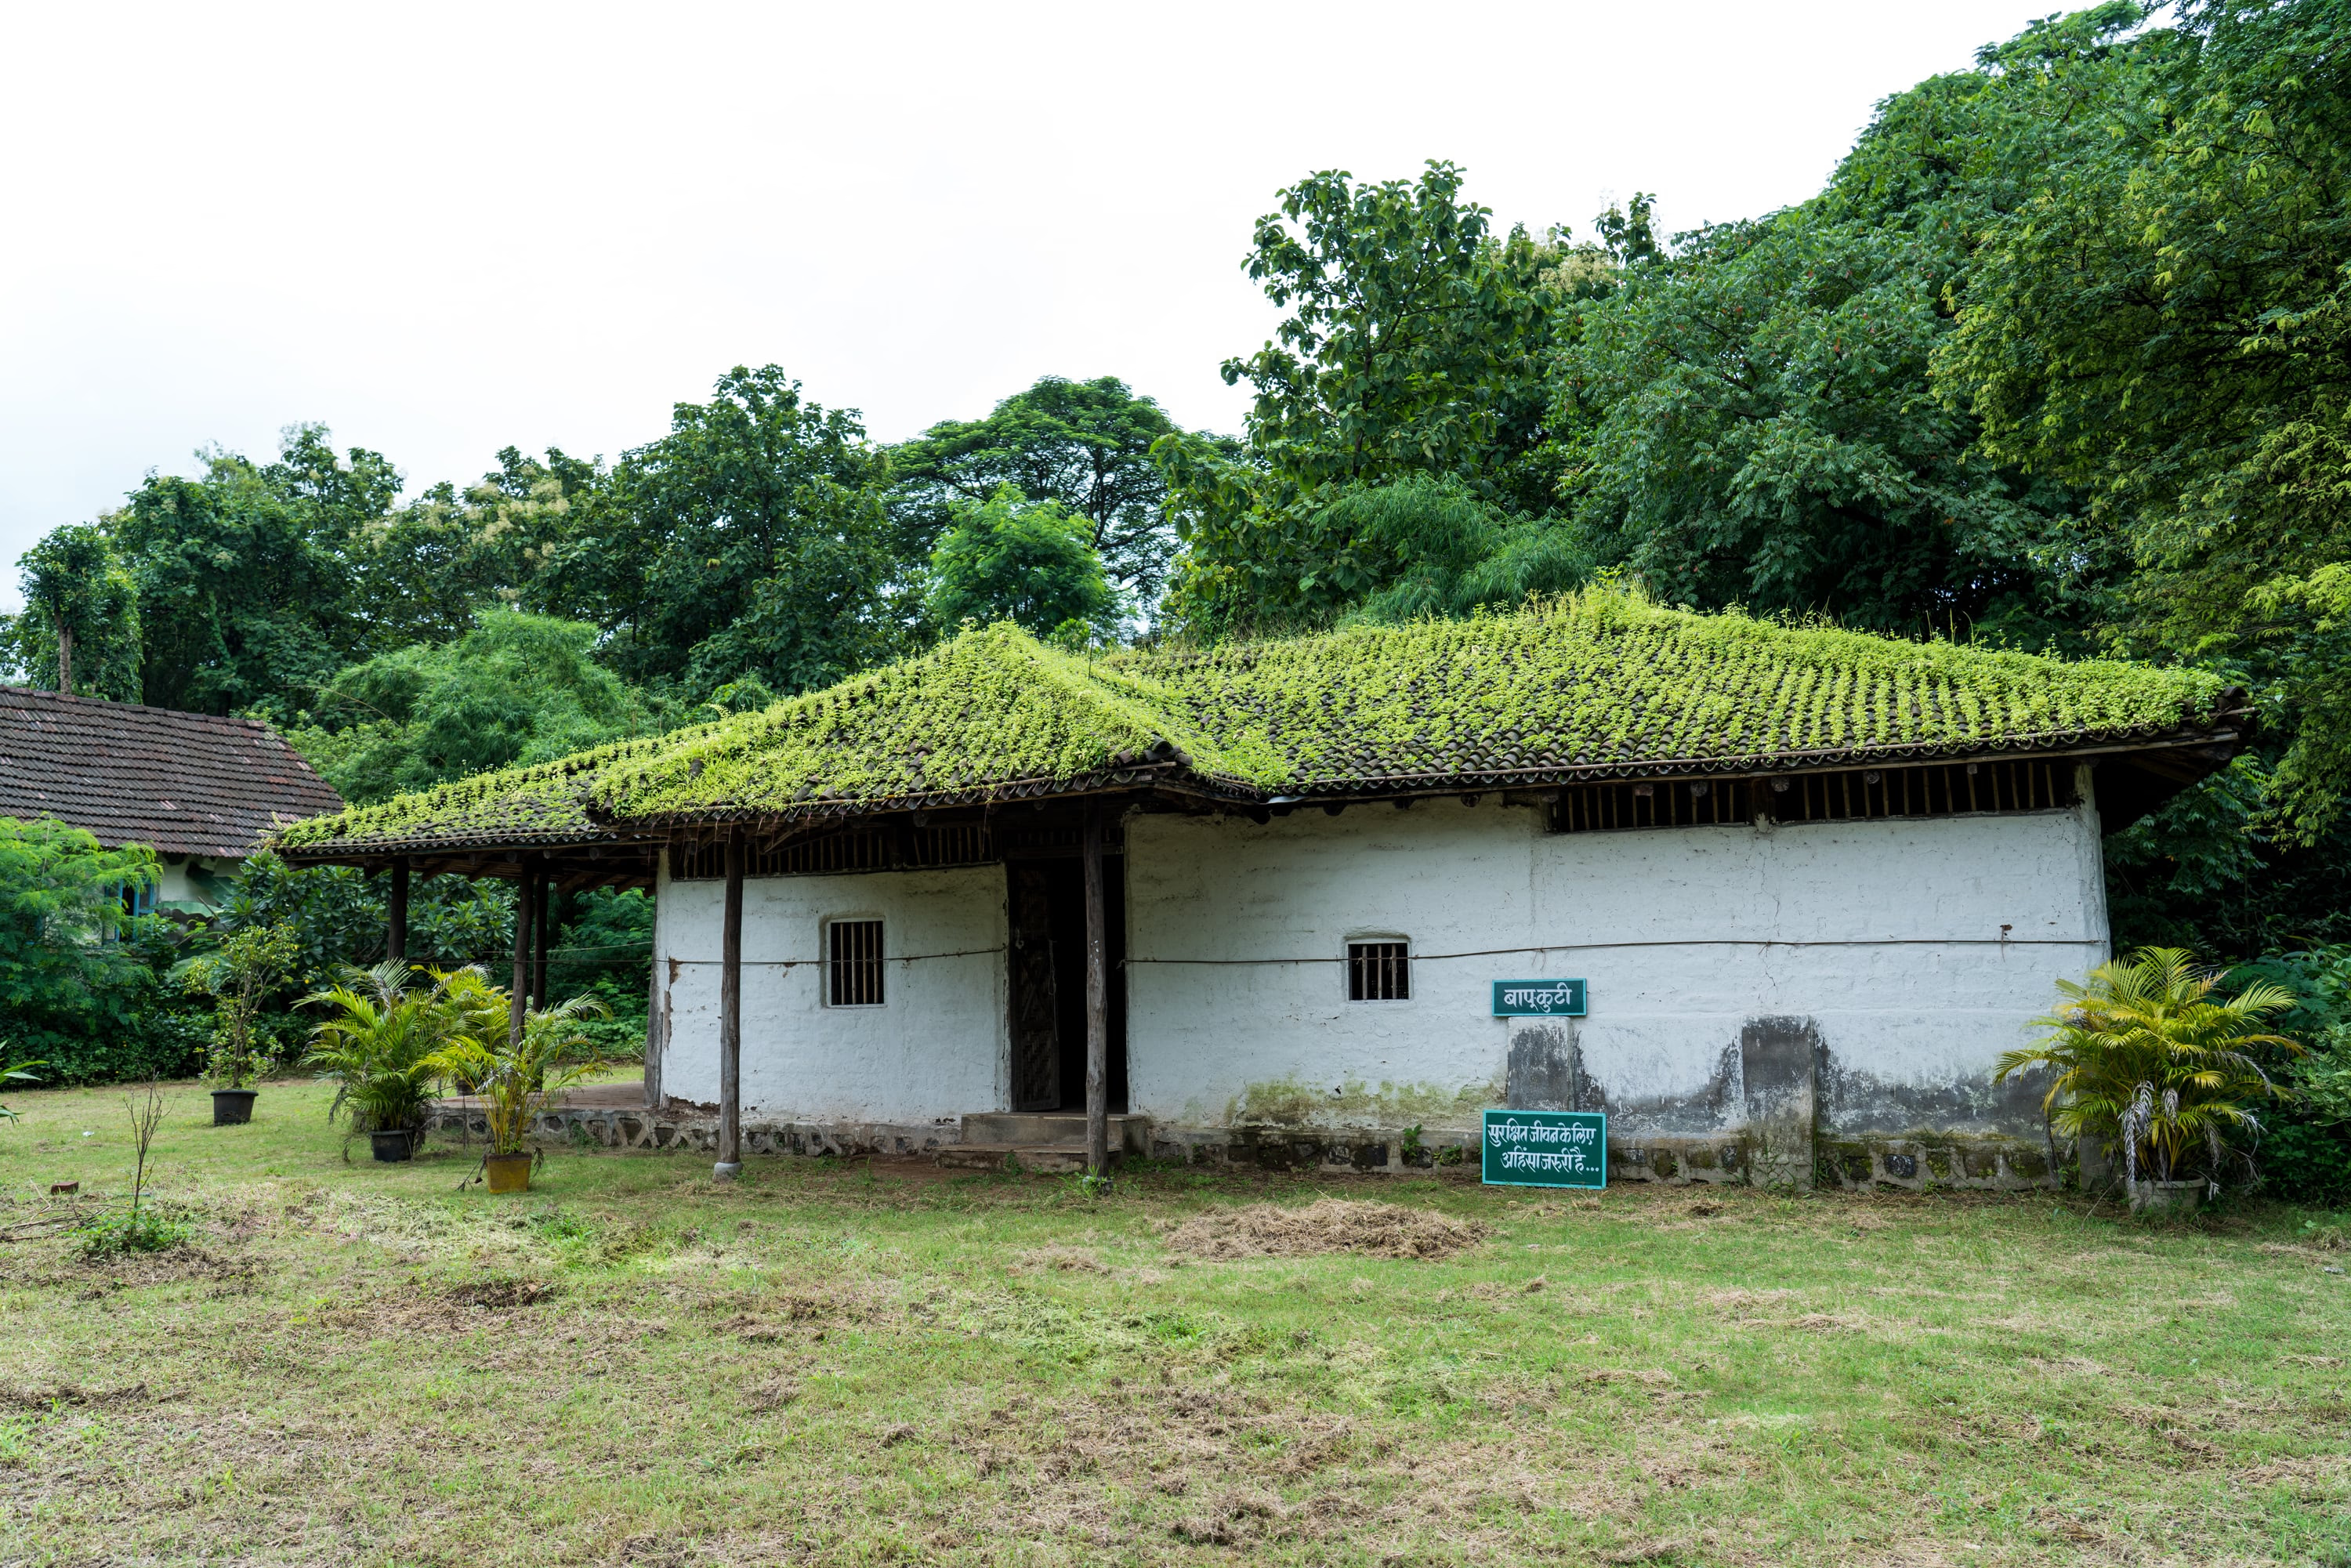
\includegraphics[width=0.8\textwidth]{bapu_kuthi1.png}
			\captionof{figure}[Bapu Kuthi]{Bapu Kuthi, created to remember the great freedom fighter Mahatma Gandhi, and to remind people of his ideologies.}
			
			\vfill
			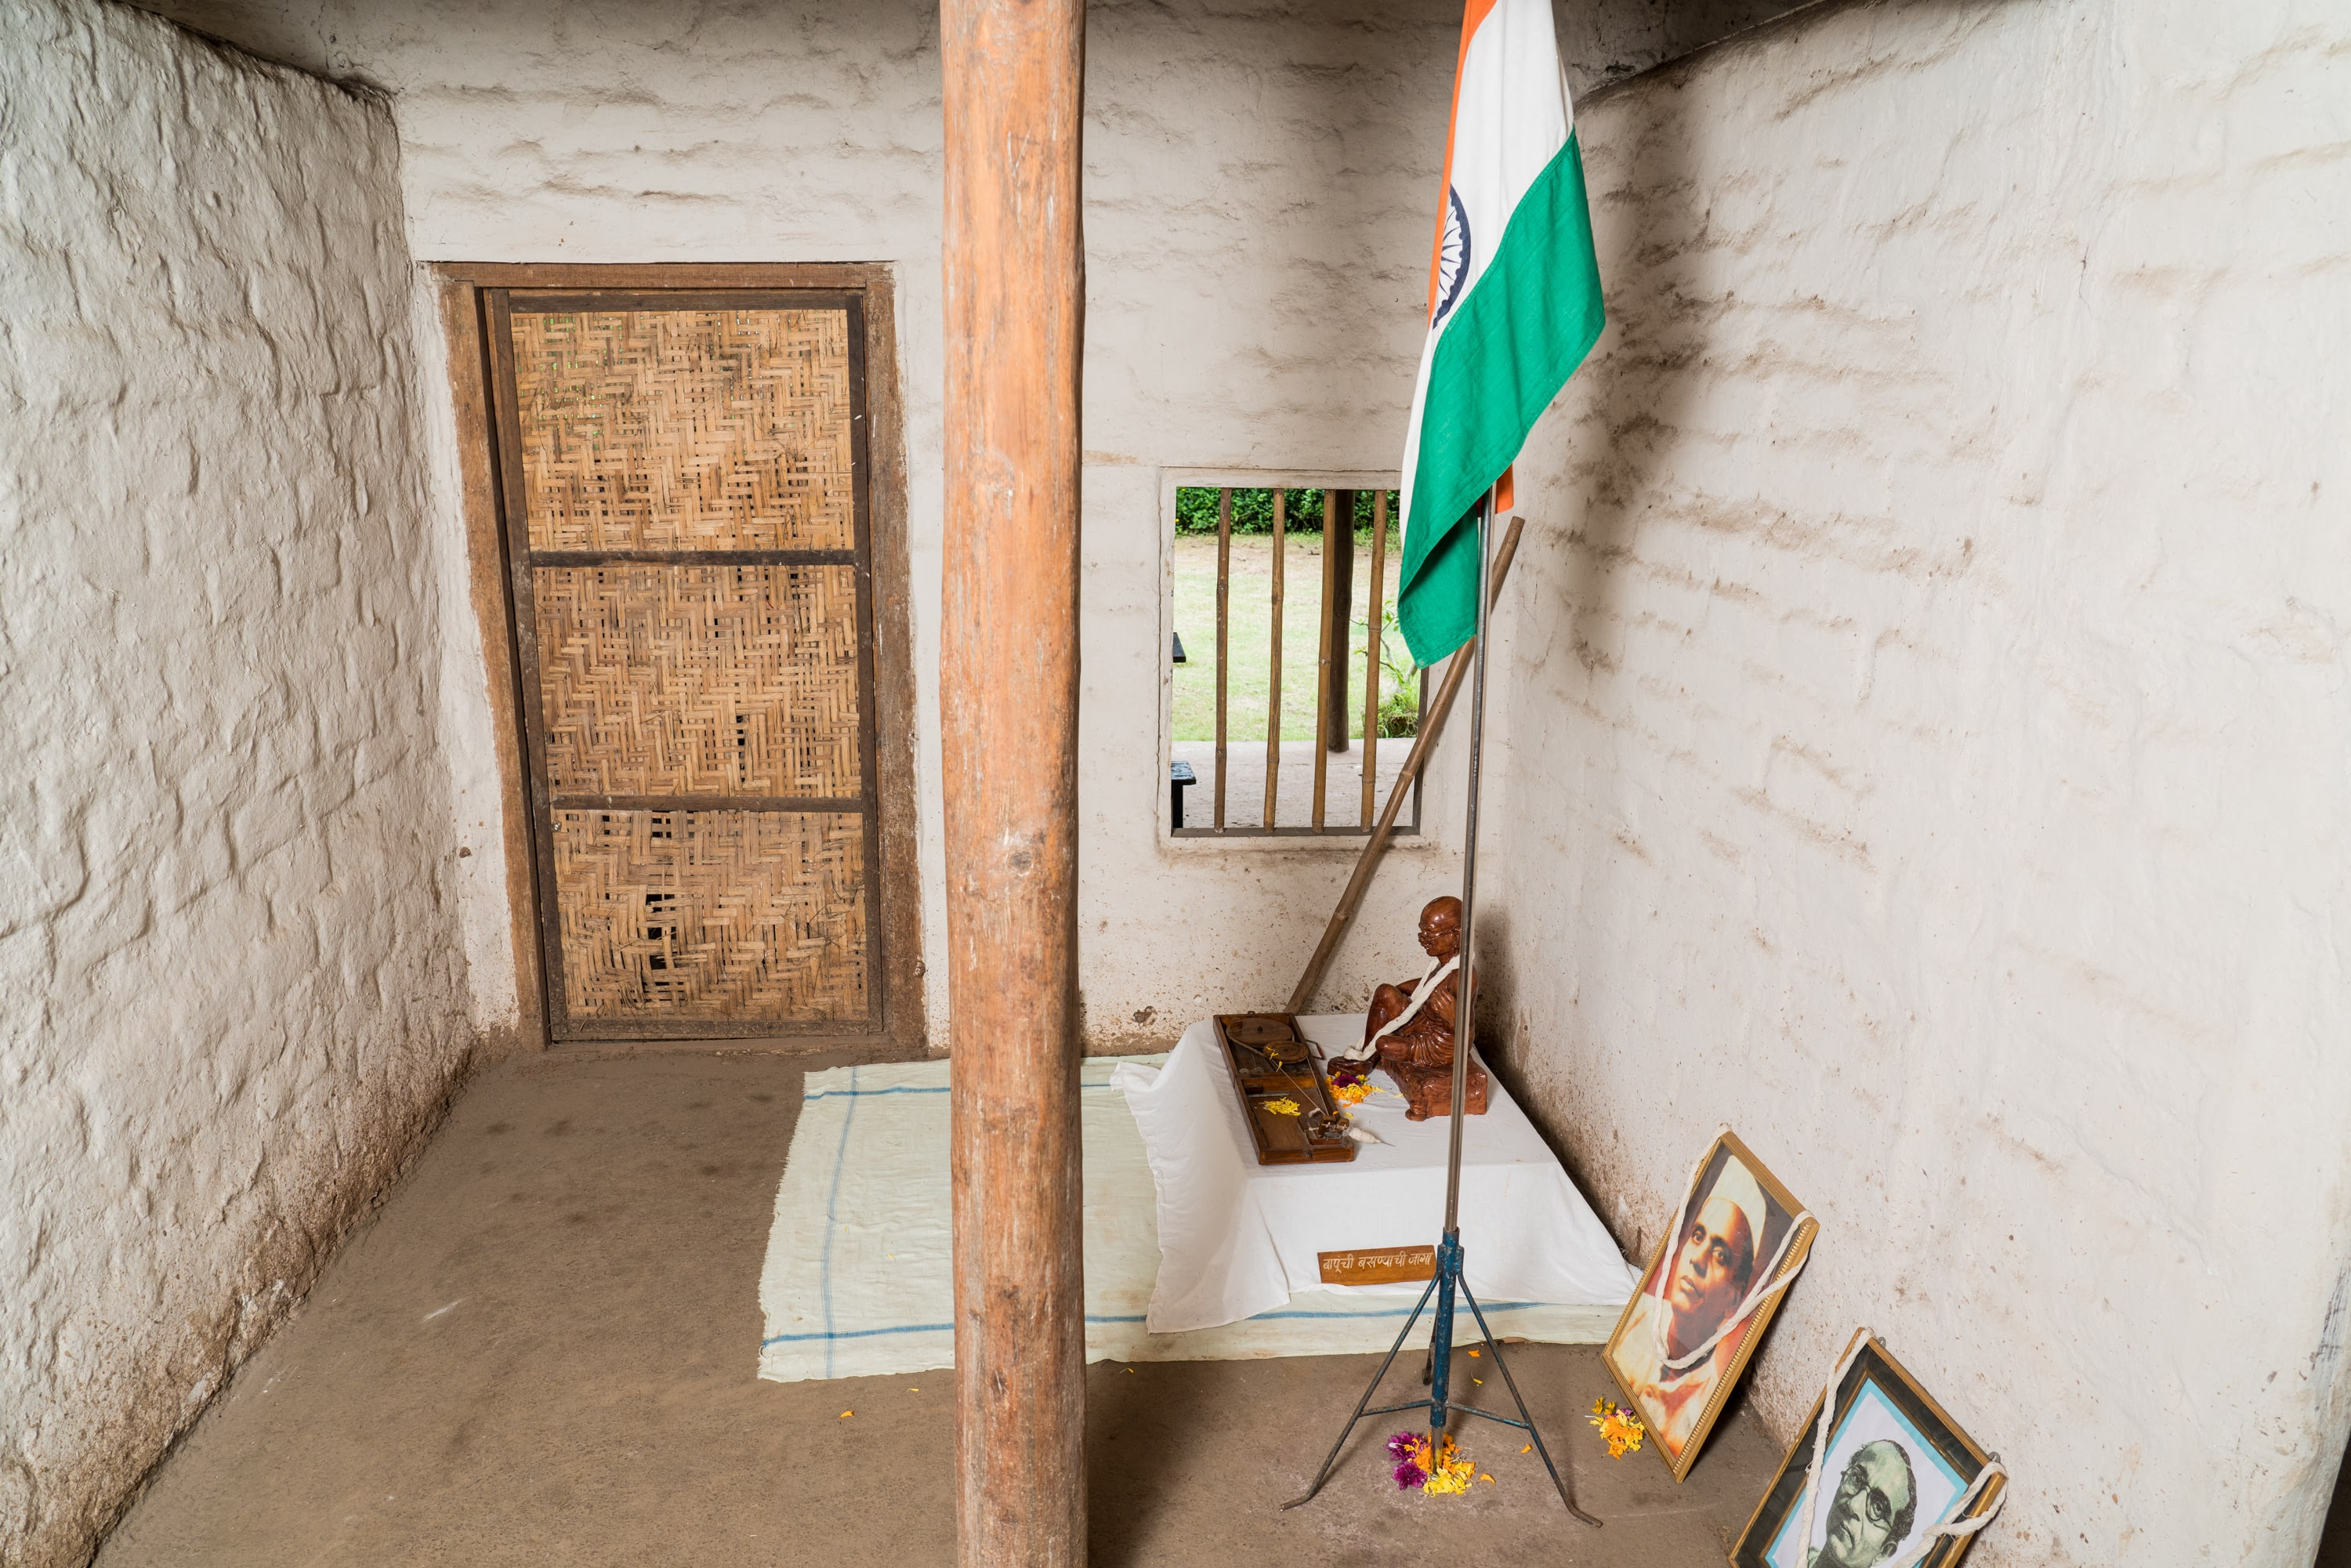
\includegraphics[width=0.8\textwidth]{bapu_kuthi2.png}
		\end{center}
		\vspace*{\fill}
		
		\clearpage
		
		\topskip0pt
		\vspace*{\fill}
		\begin{center}
			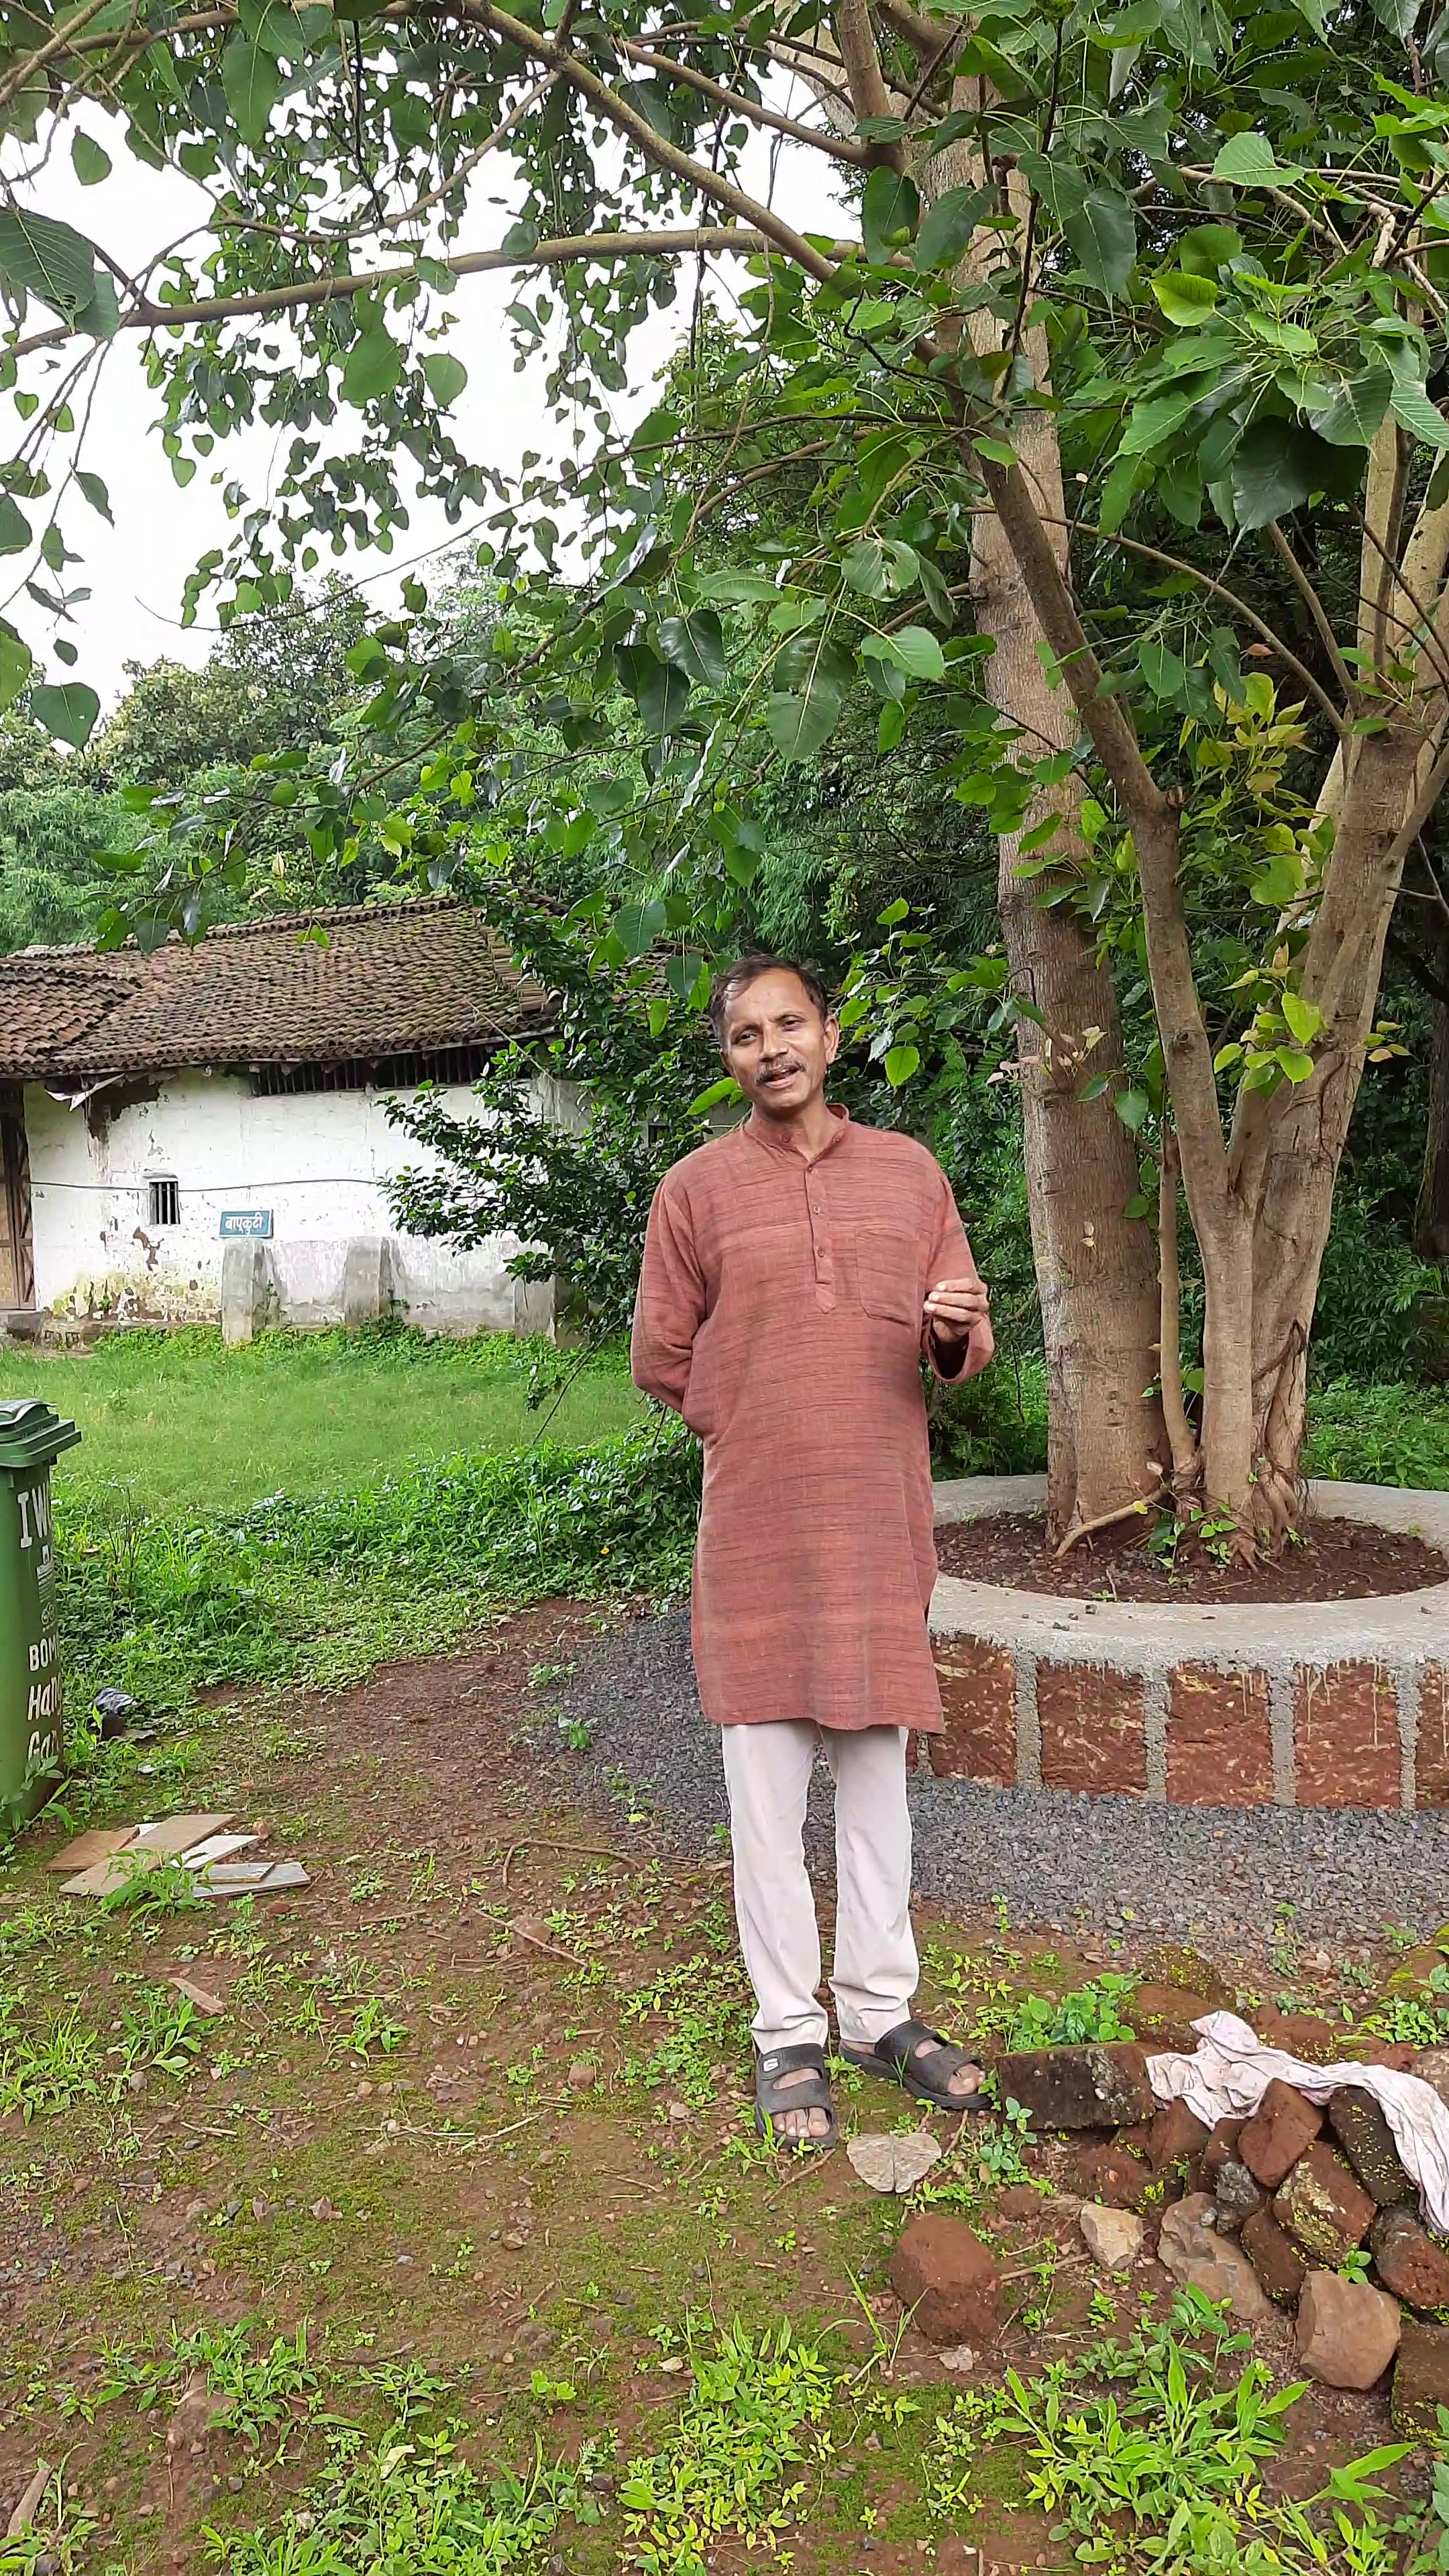
\includegraphics[width=0.7\textwidth]{bapu_kuthi3.png}
			\captionof{figure}[]{Devidas Sir explaining the aim of Bapu Kuthi.}
		\end{center}
		\vspace*{\fill}
		
		
	
\end{document}

